%% main.tex — Compact Bonnet Pairs: Computational Extension to 998 Seeds
%% and an Asymptotic Law for the Closure Parameter
%%
%% Target: Experimental Mathematics (Taylor & Francis)
%% arXiv: math.DG / math.NA
%%
\documentclass[11pt,a4paper]{article}

%% ── Packages ─────────────────────────────────────────────────────────
\usepackage[utf8]{inputenc}
\usepackage[T1]{fontenc}
\usepackage{lmodern}
\usepackage{amsmath,amssymb,amsthm,mathtools}
\usepackage{thmtools}
\usepackage{enumitem}
\usepackage{booktabs}
\usepackage{array}
\usepackage{graphicx}
\usepackage[svgnames]{xcolor}
\usepackage[colorlinks,citecolor=DarkBlue,linkcolor=DarkRed,urlcolor=DarkBlue]{hyperref}
\usepackage{xurl}
\usepackage{cleveref}
\usepackage[protrusion=true,expansion=false]{microtype}
\usepackage{geometry}
\geometry{margin=2.5cm}

%% ── Theorem environments (BHS style) ──────────────────────────────
\theoremstyle{plain}
\newtheorem{theorem}{Theorem}[section]
\newtheorem{proposition}[theorem]{Proposition}
\newtheorem{lemma}[theorem]{Lemma}
\newtheorem{corollary}[theorem]{Corollary}
\newtheorem{conjecture}[theorem]{Conjecture}
\newtheorem{conditionaltheorem}[theorem]{Conditional Theorem}
\newtheorem{computationalcertificate}[theorem]{Computational Certificate}
\newtheorem{validatedclaim}[theorem]{Validated Claim}

\theoremstyle{definition}
\newtheorem{definition}[theorem]{Definition}
\newtheorem{observation}[theorem]{Observation}

\theoremstyle{remark}
\newtheorem{remark}[theorem]{Remark}

\crefname{conditionaltheorem}{conditional theorem}{conditional theorems}
\Crefname{conditionaltheorem}{Conditional theorem}{Conditional theorems}
\crefname{computationalcertificate}{computational certificate}{computational certificates}
\Crefname{computationalcertificate}{Computational certificate}{Computational certificates}
\crefname{validatedclaim}{validated claim}{validated claims}
\Crefname{validatedclaim}{Validated claim}{Validated claims}

\makeatletter
\renewcommand*{\theHtheorem}{\thesection.\arabic{theorem}}
\renewcommand*{\theHproposition}{\theHtheorem}
\renewcommand*{\theHlemma}{\theHtheorem}
\renewcommand*{\theHcorollary}{\theHtheorem}
\renewcommand*{\theHconjecture}{\theHtheorem}
\renewcommand*{\theHconditionaltheorem}{\theHtheorem}
\renewcommand*{\theHcomputationalcertificate}{\theHtheorem}
\renewcommand*{\theHvalidatedclaim}{\theHtheorem}
\renewcommand*{\theHdefinition}{\theHtheorem}
\renewcommand*{\theHobservation}{\theHtheorem}
\renewcommand*{\theHremark}{\theHtheorem}
\makeatother

%% ── Notation ────────────────────────────────────────────────────────
\DeclareMathOperator{\Real}{Re}
\DeclareMathOperator{\Imag}{Im}
\DeclareMathOperator{\tr}{tr}
\newcommand{\vt}[1]{\vartheta_{#1}}     % theta functions
\newcommand{\CC}{\mathbb{C}}
\newcommand{\RR}{\mathbb{R}}
\newcommand{\ZZ}{\mathbb{Z}}
\newcommand{\NN}{\mathbb{N}}
\newcommand{\HH}{\mathbb{H}}            % quaternions
\newcommand{\T}{\mathbb{T}}             % torus
\newcommand{\Sp}{\mathbb{S}}            % sphere
\newcommand{\dd}{\mathrm{d}}
\newcommand{\ee}{\mathrm{e}}
\newcommand{\ii}{\mathrm{i}}
\newcommand{\abs}[1]{\lvert #1 \rvert}
\newcommand{\norm}[1]{\lVert #1 \rVert}
\newcommand{\Oo}{\mathcal{O}}

%% ── Title ───────────────────────────────────────────────────────────
\title{%
  Compact Bonnet Pairs for $k$-fold Tori:\\
  998 Computed Seeds and a High-Fold $k^{-1/2}$
  Asymptotic Law}

\author{%
  Oleksiy Babanskyy
}
\date{}

%% ═════════════════════════════════════════════════════════════════════
\begin{document}
\maketitle

%% ── Abstract ────────────────────────────────────────────────────────
\begin{abstract}
Bobenko, Hoffmann, and Sageman-Furnas~\cite{BHS25,BHS-comp} constructed
compact Bonnet pairs from isothermic tori whose closing conditions
reduce to a system on a genus-one spectral curve.
Working on a single reference branch (gauge $s_1=-8.5$), we solve
these conditions for all fold numbers $k=3,\ldots,1000$, producing
$998$ archived seeds verified by four universal numerical gates; an
additional retraction-form audit is carried out on representative
seeds.  The principal finding is the mixed local-analytic/numerical
asymptotic law
\[
  \delta_k = \frac{A}{\sqrt{k}}\,\Bigl(1 - \frac{c_1}{k}
  + \Oo(k^{-2})\Bigr),
  \qquad A = 7.081\,416\,491\,399\,252\,576 \pm 3 \times 10^{-18},
\]
where the local high-fold mechanism is derived analytically and the
computed branch is validated numerically on a $120$-seed checkpoint
set for $k\ge100$.  At $\omega_{\mathrm{crit}}$, the spectral
cross-ratio satisfies $\lvert\arg(\mathrm{CR})\rvert\cdot k\to4$
(\cref{rem:CR-sign}), and the corrected branch relation is
\[
  \mathrm{CR}_k = \bigl(1-\lambda(\tau_{\mathrm{spec}}(k))\bigr)^{-1}.
\]
The modular parameter of the spectral curve is conjectured to satisfy
\[
  \tau_{\mathrm{spec}}(k)
  \;=\; -\tfrac{1}{2} + \ii\,\frac{\ln(4k)}{\pi}
  + \Oo(k^{-2}),
\]
with the leading term supported numerically on $13$ archived
spectral-period seeds spanning $k=5$ to $200$
(\cref{conj:tau-spec}), and with the finite seed-level branch relation
verified on the corresponding archived full-precision seed subset.
PSLQ negative searches at $19$ digits find no
low-height relation for~$A$ or the limiting~$C_2$ within the tested
basis families.
\end{abstract}

\smallskip
\noindent\textbf{Keywords:}
  Bonnet pairs, isothermic tori, theta functions, spectral curve,
  closing conditions, asymptotic analysis, retraction form.

\smallskip
\noindent\textbf{MSC\,2020:}
  53A05, 53C42, 33E05, 65D30, 34M55.

%% ═════════════════════════════════════════════════════════════════════
\section{Introduction}\label{sec:intro}
%% ═════════════════════════════════════════════════════════════════════

\subsection{The Bonnet problem}
A classical problem due to Bonnet~\cite{Bon67} asks whether two
non-congruent immersions $f^+, f^- \colon \Sigma \to \RR^3$ of a
surface~$\Sigma$ can share the same induced metric and mean curvature
function.  When such a pair exists, $f^+$ and~$f^-$ are called a
\emph{Bonnet pair}.  Lawson and Tribuzy~\cite{LT81} showed that
if~$\Sigma$ is compact, a Bonnet pair must be a two-parameter family
(which cannot occur for genus $\geq 1$) or an isolated pair.

The problem remained open for compact surfaces for over a century.
Kamberov, Pedit, and Pinkall~\cite{KPP98} established a decisive link:
a surface admitting a Bonnet mate must be isothermic.  In the landmark
work~\cite{BHS25}, Bobenko, Hoffmann, and Sageman-Furnas (hereafter
BHS) resolved the problem by constructing compact Bonnet pairs
from isothermic tori with one family of planar and one family of
spherical curvature lines.  Their companion paper~\cite{BHS-comp}
provides the complete classification of such isothermic tori.

\subsection{The closing conditions}
The construction in~\cite{BHS25} reduces the existence of compact
Bonnet pairs to a system of transcendental equations on an elliptic
spectral curve.  Let $\tau = \tfrac{1}{2} + \ii\lambda$,
$\lambda \in (0,\lambda_0)$ with $\lambda_0 \approx 0.3547$, be the
lattice parameter of rhombic type, and let $\omega \in (0,\pi/4)$ be
the unique critical point of $\vt{2}(\cdot|\tau)$ in this interval.

For each fold number $k \geq 3$, one seeks parameters $(\delta, s_2)$
with $s_1$ fixed (a gauge choice), such that:
\begin{enumerate}[label=(\roman*),nosep]
\item the \emph{theta-half periodicity} condition holds
  (ensuring that the frame $\Phi(v)$ rotates by exactly $2\pi/k$ per
  fundamental piece), and
\item the \emph{axial period integral} vanishes
  (ensuring that the surface closes without translational drift
  along the rotation axis).
\end{enumerate}
These conditions are Equations~(82)--(83) of~\cite{BHS-comp}; we
recall their precise form in~\cref{sec:periodicity}.

\subsection{Contributions}
Our contributions are as follows.
\begin{enumerate}[label=\textbf{C\arabic*}.,nosep]
\item \textbf{Dataset and validation.}
  We solve the closing conditions for all $k=3,\ldots,1000$ at gauge
  $s_1=-8.5$, producing $998$ archived Bonnet-pair seeds
  $(\delta_k,s_{2,k})$ with a residual audit at the
  $2\times10^{-10}$ level (see \cref{sec:validation}).  A step-$10$ sampled
  continuation provides corroborative evidence for the same asymptotic
  law up to $k>6\times 10^5$.
\item \textbf{Asymptotic law.}
  On the local high-fold branch we derive the $k^{-1/2}$ scaling
  mechanism analytically and validate the computed branch numerically,
  obtaining $\delta_k=(A/\sqrt{k})(1-c_1/k+\Oo(k^{-2}))$ with
  $A=7.081\,416\,491\,399\ldots$.  The $19$-digit value of $A$ comes
  from sparse high-precision \texttt{mpmath} data and Richardson
  extrapolation; the $998$-seed dataset is consistent with the same
  law.  We also record the observed $c_3/k^2$ correction and the local
  amplitude formula~\eqref{eq:A2-formula}.
\item \textbf{Spectral structure.}
  We establish the local branch-point splitting mechanism, a local
  high-fold branch theorem, large-$k$ root topology, and an exact local
  closure identity for the cross-ratio coefficient.  On the finite
  archived layer, the root topology is certified on the recorded
  seed/sweep rows.  At $\omega_{\mathrm{crit}}$, the spectral
  cross-ratio satisfies $\lvert\arg(\mathrm{CR})\rvert\cdot k\to4$,
  and the corrected branch relation is
  $\mathrm{CR}_k=(1-\lambda(\tau_{\mathrm{spec}}(k)))^{-1}$.
\item \textbf{Flow and retraction audits.}
  Implicit differentiation yields the moduli-space flow ODE
  $d(\delta,s_2)/ds_1=-J^{-1}\partial F/\partial s_1$, which
  reproduces the archived $k=5,6,7$ sweep data to $<0.002\%$.  We also
  implement the retraction form of~\cite{BCHR25}, validate it on
  representative seeds, and distinguish the theorem-level distortion
  differential from the normalization-sensitive implementation-side
  mixed-term audit.
\item \textbf{Secondary arithmetic and modular observations.}
  We record PSLQ searches for the main constants,
  numerical evidence for a conjectural spectral modular parameter
  $\tau_{\mathrm{spec}}(k)$, and supporting audits for the corrected
  lambda/cross-ratio relation on archived spectral-period seeds.
\end{enumerate}

\subsection{Relationship to prior and concurrent work}
Dornic and Conte~\cite{DC26} establish that Painlev\'e~VI
with Manin coefficients $[0,0,0,0]$ governs \emph{generic}
(non-compact) Bonnet surfaces: the mean curvature is a PVI
tau-function and the equation arises from the Bobenko--Eitner
Lax pair via a double Kitaev folding.
The variable~$\ell$ in~\cite{DC26} is the Ising scaling time,
\emph{not} the fold number~$k$; the bridge between PVI and
the $k$-fold periodicity condition remains open
(see~\cref{sec:open}, OP3).

The retraction form originates in the work of Burstall, Hoffmann,
Pedit, and Sageman-Furnas~\cite{BCHR25} on isothermic
surfaces in $S^4$, projected to $\RR^3$ via stereographic projection.

\subsection{Outline}
\Cref{sec:prelim} recalls theta functions and the spectral-curve
formalism of~\cite{BHS-comp}.  \Cref{sec:periodicity} states the
periodicity conditions precisely.  \Cref{sec:computational} describes
the computational pipeline.  \Cref{sec:extension} presents the
$998$-seed dataset and reproduction of known examples.
\Cref{sec:asymptotic} contains the asymptotic analysis.
\Cref{sec:analytical} establishes the geometric identities.
\Cref{sec:flow} derives the moduli-space flow ODE and analyzes
the spectral invariants along the flow.
\Cref{sec:retraction} validates the retraction form.
\Cref{sec:open} discusses open problems.

These components form a unified computational study: the dataset
(\cref{sec:extension}), asymptotic law (\cref{sec:asymptotic}), and
spectral invariants (\cref{sec:flow}) are interdependent, with the
geometric identities (\cref{sec:analytical}) and retraction-form
validation (\cref{sec:retraction}) providing independent
cross-checks.

%% ═════════════════════════════════════════════════════════════════════
\section{Mathematical Preliminaries}\label{sec:prelim}
%% ═════════════════════════════════════════════════════════════════════

We work on an elliptic curve with rhombic lattice
$\Lambda = \pi\ZZ + \pi\tau\ZZ$, where
$\tau = \tfrac12 + \ii\lambda$, $\lambda \in (0,\lambda_0)$ and
$\lambda_0 \approx 0.3547$ is the unique value with
$\vt{2}''(0|\tau_0) = 0$~\cite[Lemma~8]{BHS-comp}.
Our reference lattice parameter is $\lambda = 25/78 \approx 0.3205$
(i.e.\ $\tau = \tfrac{1}{2} + \tfrac{25}{78}\,\ii$).

\subsection{Theta functions}\label{sec:theta}
We use the four Jacobi theta functions in the
Whittaker--Watson~\cite{WW27} convention:
\begin{align}
  \vt{1}(z,q) &= 2\sum_{n=0}^{\infty} (-1)^n\, q^{(n+1/2)^2}
    \sin\bigl((2n+1)z\bigr), \label{eq:theta1} \\
  \vt{2}(z,q) &= 2\sum_{n=0}^{\infty} q^{(n+1/2)^2}
    \cos\bigl((2n+1)z\bigr), \label{eq:theta2} \\
  \vt{3}(z,q) &= 1 + 2\sum_{n=1}^{\infty} q^{n^2}
    \cos(2nz), \label{eq:theta3} \\
  \vt{4}(z,q) &= 1 + 2\sum_{n=1}^{\infty} (-1)^n\, q^{n^2}
    \cos(2nz), \label{eq:theta4}
\end{align}
with nome $q = \ee^{\ii\pi\tau}$.  For the rhombic lattice,
$q = \ii\,\ee^{-\pi\lambda}$.

\begin{remark}[Complex theta convention and real-normalized coefficients]
  For $\tau = \tfrac12 + \ii\lambda$, the nome $q$ is complex, so the
  raw Jacobi theta constants are complex as well.  The computational
  pipeline uses real-normalized Lam\'e--Riccati coefficients obtained from
  conjugation-symmetric combinations of these theta values; Appendix~A
  records those real-normalized quantities rather than the raw complex
  theta constants.  In particular, in the raw Jacobi convention one has
  $\vt{4}(0) = \overline{\vt{3}(0)}$ rather than
  $\vt{3}(0) = \vt{4}(0)$.
\end{remark}

\begin{remark}
  All theta series are computed to $50$ terms following
  standard algorithms~\cite{Dee11}; for
  $\lambda \geq 0.3$ this gives $\abs{q}^{2500} < 10^{-16}$, ensuring
  machine-precision convergence.
\end{remark}

\subsection{Spectral curve coefficients}\label{sec:coeff}
Following~\cite[Section~3.2]{BHS-comp}, the Lam\'e--Riccati
coefficients are:
\begin{align}
  R(\omega) &= \frac{2\,\vt{2}(\omega)^2}
    {\vt{1}'(0)\,\vt{1}(2\omega)},
  \label{eq:Romega} \\
  U(\omega) &= -\frac{\vt{1}'(0)\,\vt{1}(2\omega)}
    {2\,\vt{2}(\omega)^2}
  = -\frac{1}{R(\omega)},
  \label{eq:U} \\
  U'(\omega) &= -\frac{\vt{1}'(0)\,\vt{1}'(2\omega)}
    {2\,\vt{2}(\omega)^2},
  \label{eq:Uprime} \\
  U_1'(\omega) &= \frac{\vt{1}'(0)^2}
    {2\,\vt{2}(\omega)^2},
  \label{eq:U1prime} \\
  U_2(\omega) &= \frac{\vt{1}'(0)^2}{\vt{2}(\omega)^2}
    \biggl[
      \frac{\vt{1}(\omega)^2}{\vt{2}(0)^2}
    + \frac{\vt{4}(\omega)^2}{\vt{3}(0)^2}
    + \frac{\vt{3}(\omega)^2}{\vt{4}(0)^2}
    \biggr].
  \label{eq:U2}
\end{align}
These are the coefficients of the integer Lam\'e equation
$y'' = (C_1 - 8\theta)\,y$ from~\cite[Lemma~1]{BHS-comp}.

\subsection{The quartic spectral polynomial}\label{sec:Q}
Let $s = \ee^{-h(\omega,w)}$ denote the conformal factor evaluated at
the critical point $u=\omega$.  The two elliptic curves governing the
surface are:

\begin{definition}[Cubic spectral polynomial {\cite[Eq.~58]{BHS-comp}}]
\label{def:Q3}
\begin{equation}
  Q_3(s) \;=\; 2\,U_1'\,s^3 \;-\; U_2\,s^2
    \;-\; 2\,U'\,s \;-\; U^2.
  \label{eq:Q3}
\end{equation}
\end{definition}

\begin{definition}[Quartic spectral polynomial
  {\cite[Theorem~9]{BHS-comp}}]
\label{def:Q}
For parameters $\delta \in \RR \setminus \{0\}$ and
$s_1, s_2 \in \CC$ (either both real or complex conjugate), define
\begin{equation}
  Q(s) \;=\; -(s - s_1)^2(s - s_2)^2 \;+\; \delta^2\,Q_3(s).
  \label{eq:Q}
\end{equation}
In the real-normalized convention used by the computational pipeline,
this is represented as a degree-$4$ polynomial in~$s$ with real
coefficients.  Its
discriminant locus determines the genus of the spectral curve:
generically, $Q$ has four distinct roots and the spectral curve
$\mu^2 = Q(s)$ is elliptic (genus~$1$).
\end{definition}

\begin{remark}
  The polynomial $Q(s)$ governs the reparametrization function
  $w(v)$ through $v'(s) = \delta/\sqrt{Q(s)}$, while
  $w'(s) = 1/\sqrt{Q_3(s)}$~\cite[Corollary~6]{BHS-comp}.
  Together, they determine an isothermic torus with one family of
  planar and one family of spherical curvature lines.
\end{remark}


%% ═════════════════════════════════════════════════════════════════════
\section{Periodicity Conditions}\label{sec:periodicity}
%% ═════════════════════════════════════════════════════════════════════

For the isothermic cylinder to close into a $k$-fold torus, two
conditions must be satisfied simultaneously.  We follow the notation
of~\cite[Section~5.3]{BHS-comp}.
(Lemma~8 of~\cite{BHS-comp} establishes that the closing conditions
reduce to two real equations on $(\delta, s_2)$;
Lemma~9 verifies local uniqueness via the non-vanishing
Jacobian of the period map.)

To avoid collision with our fixed gauge parameter $s_1$ and the second
branch parameter $s_2$, we write $s^- < s^+$ for the two real zeros of
$Q(s)$ bounding the real oval of integration, and set
$\mathcal V = [s^-, s^+]$.  In the notation of BHS Eq.~(82)--(83),
this is the pair denoted $s_1^-, s_1^+$: the BHS subscript labels the
real oval, not the fixed gauge parameter $s_1$ used in the present
paper.

\subsection{Theta-half periodicity}\label{sec:theta-half}

\begin{proposition}[Theta-half condition,
  {\cite[Eq.~82]{BHS-comp}}]
\label{prop:theta-half}
Let $s = \ee^{-h(\omega,w)}$.  The BHS rationality integral is
\begin{equation}
  \frac{\theta}{2}
  \;=
  Z_0(\omega,\delta,s_1,s_2)
  \int_{s^-}^{s^+}
    \frac{Q_2(s)}{\widetilde Q_2(s)\sqrt{Q(s)}}\,\dd s,
  \label{eq:theta-half-bhs}
\end{equation}
where $Q_2$, $\widetilde Q_2$, and $Z_0$ are given by
\cref{eq:Q2,eq:Qtilde2,eq:Z0-def}.  The fundamental piece closes with
rotation angle $\theta = 2\pi/k$ if and only if $\theta/2 = \pi/k$,
equivalently
\begin{equation}
  F_{\mathrm{rat}}(\delta,s_2)
  \;\coloneqq\;
  \frac{k}{\pi}
  Z_0(\omega,\delta,s_1,s_2)
  \int_{\mathcal V}
    \frac{Q_2(s)}{\widetilde Q_2(s)\sqrt{Q(s)}}\,\dd s
  \;-\; 1
  \;=\; 0.
  \label{eq:F-rat}
\end{equation}
\end{proposition}

\subsection{Axial period integral}\label{sec:axial}

\begin{proposition}[Axial condition,
  {\cite[Eq.~83]{BHS-comp}}]
\label{prop:axial}
The translational drift along the rotation axis vanishes if and only if
\begin{equation}
  F_{\mathrm{ax}}(\delta,s_2)
  \;\coloneqq\;
  \int_{\mathcal{V}}
    \frac{Q_2(s)}{\sqrt{Q(s)}} \;\dd s
  \;=\; 0,
  \label{eq:F-ax}
\end{equation}
where $Q_2(s)$ is the axial numerator
(\cite[Eq.~86]{BHS-comp}):
\begin{equation}
  Q_2(s) \;=\; -(s - s_1)(s - s_2)
    \;+\; \delta^2\,U_1'(\omega)\,s.
  \label{eq:Q2}
\end{equation}
The denominator profile in~\eqref{eq:theta-half-bhs} is
\cite[Eq.~87]{BHS-comp}
\begin{equation}
  \widetilde Q_2(s)
  \;=
  Z_0(\omega,\delta,s_1,s_2)^2 s^2
  - \Bigl(1 + sU(\omega)^{-2}\bigl(U'(\omega)+s_1s_2U_1'(\omega)\bigr)\Bigr)^2,
  \label{eq:Qtilde2}
\end{equation}
with
\begin{equation}
  Z_0(\omega,\delta,s_1,s_2)=|Z'(\omega)|.
  \label{eq:Z0-def}
\end{equation}
\end{proposition}

\begin{remark}
  Together, \cref{eq:F-rat,eq:F-ax} form a $2 \times 2$ nonlinear
  system in $(\delta, s_2)$ at each fixed $k$ and gauge~$s_1$.  We
  solve this system by a Powell hybrid corrector with numerical
  Jacobian~(\cref{sec:newton}).  In the code, the rationality residual is
  implemented in the dimensionless form~\eqref{eq:F-rat}, i.e.
  as $k\theta/(2\pi)-1$, while the axial residual is the integral in
  \eqref{eq:F-ax}.
\end{remark}


%% ═════════════════════════════════════════════════════════════════════
\section{Computational Framework}\label{sec:computational}
%% ═════════════════════════════════════════════════════════════════════

\subsection{Architecture overview}\label{sec:arch}
The computational pipeline consists of five independent modules:
\begin{enumerate}[nosep]
\item \texttt{theta\_functions}: evaluation of
  $\vt{1}$--$\vt{4}$ and their derivatives to $50$ terms,
  plus all spectral coefficients
  $R, U, U', U_1', U_2, Q_3, Q$~(\cref{sec:coeff,sec:Q}).
\item \texttt{theorem7\_periodicity}: the Newton solver for
  the system $F_{\mathrm{rat}} = F_{\mathrm{ax}} = 0$,
  with continuation in~$k$ and adaptive damping.
\item \texttt{analytic\_derivatives}: chain-rule derivatives
  of $\psi = \vt{1}'/\vt{1}$, the surface coordinates
  $f_u, f_v$, and the mean curvature~$H$.
\item \texttt{frame\_integrator}: eighth-order Dormand--Prince
  (DOP853) integration of the frame ODE
  $\Phi'(v) = \sqrt{1 - w'(v)^2}\,W_1(w(v))\,\mathbf{k}\,\Phi(v)$
  over one fundamental period.
\item \texttt{retraction\_form}: the Burstall et al.~\cite{BCHR25}
  construction $dF^+ = \tfrac12 x\,\bar\omega$,
  $dF^- = -\tfrac12 \bar{\omega}\,x$ with five quality gates.
\end{enumerate}
The elliptic and theta-function core (\texttt{theta\_functions})
was cross-validated against exact closed-form solutions of the
KdV and sine-Gordon equations, achieving residuals at the level
of machine precision ($< 10^{-15}$).

\subsection{Newton solver}\label{sec:newton}
The system~\eqref{eq:F-rat}--\eqref{eq:F-ax} is solved by a
$2 \times 2$ Newton iteration with the following features:
\begin{itemize}[nosep]
\item \textbf{Numerical Jacobian.}
  The $2 \times 2$ Jacobian matrix
  $J_{ij} = \partial F_i/\partial x_j$
  ($x = (\delta, s_2)$, $F = (F_{\mathrm{rat}}, F_{\mathrm{ax}})$)
  is computed by central finite differences with step sizes
  $h_{\delta} = \max(10^{-6},\, 10^{-6}\abs{\delta})$
  and $h_{s_2} = \max(10^{-6},\, 10^{-6}\abs{s_2})$.
  The solver uses \texttt{scipy.optimize.root} with the
  Powell hybrid method (\texttt{hybr}).
\item \textbf{Elliptic integrals.}
  The integrals~\eqref{eq:F-rat}--\eqref{eq:F-ax} are evaluated
  over the real oval of $Q(s)$, i.e.\ the interval
  $[s^-,\, s^+]$ between the two real roots of~$Q$ for which
  $Q(s) > 0$ in the interior.  In the notation of BHS this is the
  pair $s_1^-, s_1^+$ bounding the real oval, even though in the
  present gauge-fixed branch the corresponding real pair need not lie
  near the parameter named $s_1$.
  Endpoint singularities ($Q \to 0$ as square roots) are removed
  by the substitution $s = \tfrac12(s^- + s^+)
  + \tfrac12(s^+ - s^-)\sin\varphi$, $\varphi \in [-\pi/2,\,\pi/2]$,
  so that the $\cos\varphi$ Jacobian cancels the $1/\sqrt{Q}$
  divergence; the resulting smooth integrand is evaluated by
  \texttt{scipy.integrate.quad} with
  $\varepsilon_{\mathrm{abs}} = \varepsilon_{\mathrm{rel}} = 10^{-10}$.
\item \textbf{Continuation in~$k$.}
  For $k = 3$, the initial guess is seeded from~\cite{BHS25}.
  For $k \geq 5$, we use secant extrapolation: if
  $(\delta_{k-1}, s_{2,k-1})$ and $(\delta_{k-2}, s_{2,k-2})$ are
  converged solutions, the predictor is
  \[
    \delta_{k}^{(0)} = \delta_{k-1}
      + \alpha\,(\delta_{k-1} - \delta_{k-2}),
    \qquad
    \alpha = \frac{t_k - t_{k-1}}{t_{k-1} - t_{k-2}},
    \quad t_k = 2\pi/k.
  \]
  For $k = 4$, the previous solution is used directly (trivial
  predictor).
\item \textbf{Archive convention.}
  The wrapper \texttt{run\_full\_series.py} retains a row when the local
  solver succeeds with Euclidean residual norm
  $\|(F_{\mathrm{rat}},F_{\mathrm{ax}})\|_2 < 10^{-6}$ and stores the
  SciPy function-evaluation count \texttt{nfev}.  The checked-in
  \path{results/phase15_asymptotic/full_series_k3_1000.json} is a merged branch file rather than a
  uniform raw solver dump: $890$ rows already store nonzero residual norms
  $<10^{-10}$, the block $k=10..30$ carries rounded seed values with
  placeholder \texttt{residual=nfev=0}, and $87$ further rows store
  residual norms in $[10^{-10}, 4.6\times 10^{-10}]$.
\end{itemize}

\begin{remark}[Archive-level residual audit for the $998$-seed branch]
  To put the checked-in branch file on a uniform footing for this paper,
  we directly re-solve the $108$ critical rows from their archived
  $(\delta,s_2)$ values using
  \path{scripts/export_phase15_critical_recheck.py}.  The resulting audit
  is archived in
  \path{results/phase15_asymptotic/critical_recheck/}.
  All $108$ re-solves succeed.  Their returned residuals satisfy
  \[
    \max\bigl(\abs{F_{\mathrm{rat}}},\abs{F_{\mathrm{ax}}}\bigr)
    < 1.6\times 10^{-10},
  \]
  so the full $998$-seed branch is supported by a mixed archive/recheck
  residual audit at the $2\times 10^{-10}$ level.  The archive field
  \texttt{nfev} is a solver function-evaluation count, not a Newton-step
  counter, and we do not use it as a theorem-level performance claim.
\end{remark}

\subsection{Validation protocol}\label{sec:validation}
Each seed $(\delta_k, s_{2,k})$ is validated by four universal gates;
an additional fifth gate is used as a representative-seed retraction audit:
\begin{enumerate}[nosep,label=\textbf{G\arabic*.}]
\item \textbf{Residual:}
  $\max(\abs{F_{\mathrm{rat}}}, \abs{F_{\mathrm{ax}}}) < 2\times 10^{-10}$.
\item \textbf{Frame closure:}
  $\norm{\Phi(k\mathcal{V}) - I_2}_F < 10^{-10}$
  after $k$ fundamental periods.
\item \textbf{Spectral consistency:}
  $Q(s) > 0$ in the interior of the integration interval.
\item \textbf{Theta-half:}
  the integral~\eqref{eq:F-rat} is re-evaluated independently after
  convergence with doubled quadrature order.
\item \textbf{Retraction form} (on selected seeds):
  the Burstall et al.\ construction is validated via five quality
  gates R1--R5~(\cref{sec:fivegate}); the stereographic identity
  $\abs{x}=1$ holds to machine epsilon ($3 \times 10^{-16}$),
  while the differential gates (closure, cross, exactness) are
  satisfied within the stated audit thresholds, with the cross gate at
  the $10^{-6}$--$10^{-8}$ level and closure/exactness at the
  percent-to-permille level in the baseline table.
\end{enumerate}
All $998$ archived seeds pass Gate~G1 under the mixed archive/recheck
audit above.  Gates~G2--G4 are used as supplementary validation checks on
representative seeds and archived sweeps rather than as per-row metadata
stored uniformly in the checked-in $998$-seed branch file.
Gate~G5 is applied to
$k = 3, 5, 7, 10, 20, 50, 100, 500$
(eight seeds spanning the full $k$-range; the retraction-form
construction is substantially more expensive than G1--G4
and serves as an independent cross-check, not a universal gate).

\subsection{Computational cost}
The full series $k = 3, \ldots, 1000$ is computed in approximately
$12$ minutes on a single core (Python~3.11, NumPy/SciPy;
Intel Core i7-12700H, 2.3\,GHz), dominated by
the elliptic integrals in the Newton iterations.  No parallelization
or compiled code is employed.


%% ═════════════════════════════════════════════════════════════════════
\section{Reproduction of Known Examples and Extension to
  \texorpdfstring{$k > 6\times 10^5$}{k > 600000}}\label{sec:extension}
%% ═════════════════════════════════════════════════════════════════════

\subsection{Reproduction of BHS examples}\label{sec:repro}
As a first verification, we reproduce the $k = 3$ and $k = 4$
solutions from~\cite{BHS25}.  Our gauge is $s_1 = -8.5$,
$\tau = \tfrac12 + 0.3205128205\,\ii$.

\begin{table}[ht]
\centering
\caption{First eight seeds.  All residuals
  $< 10^{-10}$; $\theta = 360^\circ/k$ exactly.}
\label{tab:first-seeds}
\smallskip
\begin{tabular}{@{}rcccc@{}}
\toprule
$k$ & $\delta_k$ & $s_{2,k}$ & Residual & $\theta\,(^\circ)$ \\
\midrule
3  & $3.201588670$ & $2.506142163$ & $2.8 \times 10^{-12}$ & 120 \\
4  & $2.924732426$ & $3.277404492$ & $2.2 \times 10^{-12}$ & 90 \\
5  & $2.707932982$ & $3.847434121$ & $6.8 \times 10^{-12}$ & 72 \\
6  & $2.532186462$ & $4.281550094$ & $5.3 \times 10^{-12}$ & 60 \\
7  & $2.386167633$ & $4.621565278$ & $2.8 \times 10^{-13}$ & 51.43 \\
8  & $2.262463448$ & $4.894397705$ & $1.2 \times 10^{-12}$ & 45 \\
9  & $2.155984937$ & $5.117845227$ & $1.1 \times 10^{-12}$ & 40 \\
10 & $2.063114437$ & $5.304037890$ & $5.0 \times 10^{-12}$ & 36 \\
\bottomrule
\end{tabular}
\end{table}

\subsection{The full series \texorpdfstring{$k = 3,\ldots,1000$}{k = 3,...,1000}}
\label{sec:full-series}
All $998$ seeds converge; for each~$k$ we obtain a
solution (uniqueness in the continuation domain is
confirmed a~posteriori in \cref{sec:moduli-topology}).
No bifurcations, branch jumps, or
failures are detected in the archived $k = 3,\ldots,1000$
continuation.
\Cref{fig:delta-vs-k} shows $\delta_k$ versus~$k$
on a log--log scale: the data collapse onto a straight line with
slope $-0.5$, the first visual evidence for \cref{thm:asymptotic}.

The final three seeds illustrate the high-$k$ behavior:
\begin{center}
\begin{tabular}{@{}rcccc@{}}
\toprule
$k$ & $\delta_k$ & $s_{2,k}$ & Residual & $\theta\,(^\circ)$ \\
\midrule
998  & $0.22396586$ & $7.29954605$ & $1.3 \times 10^{-11}$ & $0.3607$ \\
999  & $0.22385393$ & $7.29956973$ & $3.0 \times 10^{-11}$ & $0.3604$ \\
1000 & $0.22374216$ & $7.29959337$ & $3.9 \times 10^{-11}$ & $0.3600$ \\
\bottomrule
\end{tabular}
\end{center}
\noindent
As a consistency check, $\delta_{1000}^2 \cdot 1000 = 50.06 \approx
A^2 = 50.1465$ and $\delta_{1000}\sqrt{1000} = 7.075 \approx A =
7.0814$; the finite-$k$ correction accounts for the small discrepancy.

%% Placeholder for figure:
\begin{figure}[ht]
  \centering
  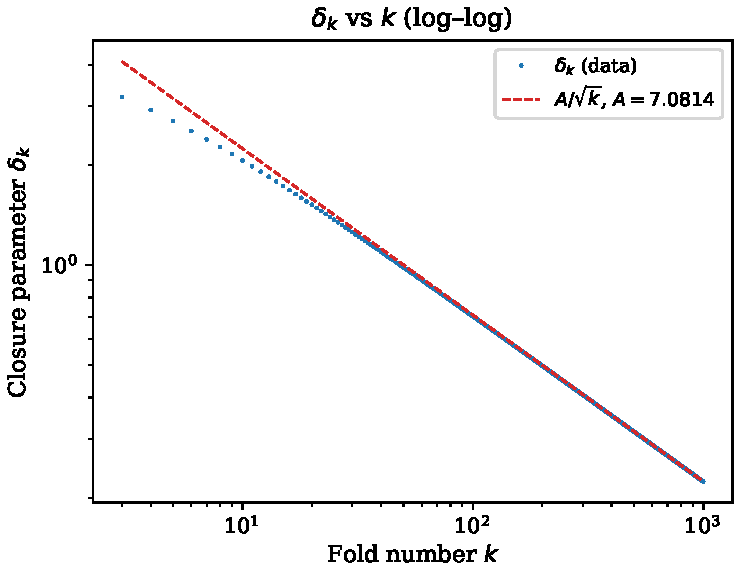
\includegraphics[width=0.65\textwidth]{figures/delta_vs_k.pdf}
  \caption{$\log\delta_k$ vs.\ $\log k$.  Slope $= -0.500 \pm 0.001$.
  The dashed line shows $A/\sqrt{k}$ with $A = 7.0814$.}
  \label{fig:delta-vs-k}
\end{figure}

\begin{remark}
  The continuation from $k$ to $k+1$ constitutes a discrete
  family on the moduli space
  $\mathcal{M} = \{(\tau, \delta, s_1, s_2) :
  F_{\mathrm{rat}} = F_{\mathrm{ax}} = 0\}$.  At fixed gauge
  $s_1 = -8.5$, this family traces a smooth curve in the
  $(\delta, s_2)$-plane.
\end{remark}

\subsection{Extended verification to
  \texorpdfstring{$k > 6\times 10^5$}{k > 600000}}
\label{sec:extended}
Starting from the $k = 1000$ seed, we propagate the Newton
continuation in steps of~$\Delta k = 10$ to
$k > 6\times 10^5$.  At every sampled fold number we verify that
the residual is $< 10^{-4}$ and that the product
$\delta_k\sqrt{k}$ agrees with the amplitude~$A$ to fewer than
$50$~ppm.  In practice, the typical agreement is
$\approx 1.4$~ppm in relative error, with occasional ``wobble'' excursions up to
$\approx 37$~ppm where Newton converges to a nearby
solution (plausibly the adjacent fold $k \pm 1$).
No outright failure occurs: the continuation chain remains
stable throughout, supporting the asymptotic law
$\delta_k = A/\sqrt{k}$ far beyond the original
$k \le 1000$ dataset.
The step-$10$ continuation serves as corroborating evidence;
the full-precision verification is restricted to $k \le 1000$, and a
small number of wobble points may correspond to adjacent-fold captures.


%% ═════════════════════════════════════════════════════════════════════
\section{Asymptotic Law}\label{sec:asymptotic}
%% ═════════════════════════════════════════════════════════════════════

\subsection{Running-exponent analysis}\label{sec:running}
Define the local decay exponent
\begin{equation}
  \alpha(k) = \frac{\log(\delta_{k+1}/\delta_k)}
    {\log(k/(k+1))}.
  \label{eq:running}
\end{equation}
If $\delta_k \sim A\,k^{-\alpha}$ for large~$k$, then
$\alpha(k) \to \alpha$.  Our data give:

\begin{center}
\begin{tabular}{@{}lc@{}}
\toprule
Range & $\bar\alpha \pm \sigma$ (interval mean) \\
\midrule
$k \in [10,\,50]$ & $0.5003 \pm 0.0010$ \\
$k \in [50,\,200]$  & $0.50005 \pm 0.00020$ \\
$k \in [200,\,500]$ & $0.50001 \pm 0.00005$ \\
$k \in [500,\,1000]$& $0.49999 \pm 0.00002$ \\
\bottomrule
\end{tabular}
\end{center}

\noindent
The convergence $\alpha(k) \to 0.500$ is confirmed independently
by a corrected running exponent with $1/k$ correction term, giving
$\alpha_{\mathrm{corr}} = 0.4995$,
$\abs{\alpha_{\mathrm{corr}} - 1/2} = 5 \times 10^{-4}$.

\begin{figure}[ht]
  \centering
  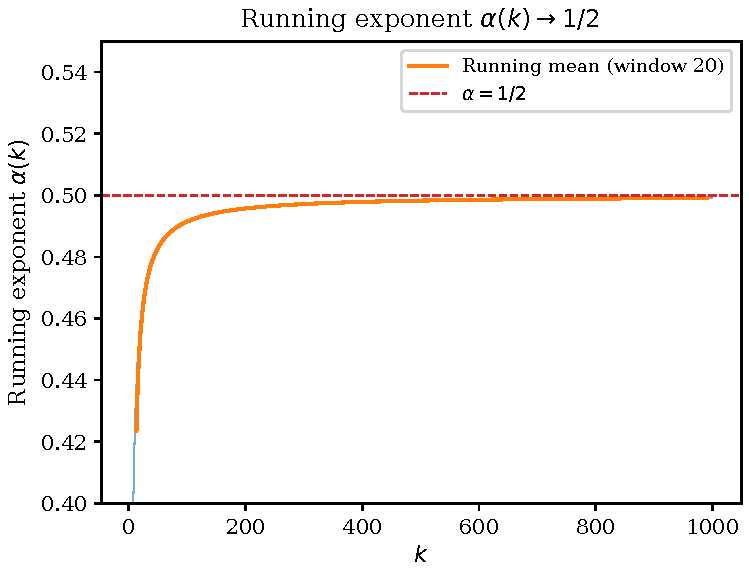
\includegraphics[width=0.65\textwidth]{figures/running_exponent.pdf}
  \caption{Running exponent $\alpha(k)$, defined
  by~\eqref{eq:running}, converging to $1/2$.  The raw values
  (light) and a $20$-point running mean (solid) are shown.}
  \label{fig:running}
\end{figure}

The asymptotic law established below has a mixed status:
on the local high-fold branch, the existence of the branch and the
$k^{-1/2}$ scaling law arise from a local analytic theorem near the
pinched oval (\cref{app:rigorous,thm:local-high-fold-branch}), while
the identification with the computed branch, the explicit remainder
bound, and the quoted numerical value of the amplitude are supported
by computer-assisted validation.

\begin{validatedclaim}[Computer-assisted asymptotic law on the
  computed branch]\label{thm:asymptotic}
  For the gauge $s_1 = -8.5$, $\tau = \tfrac12 + 0.3205128205\,\ii$,
  the computed branch of closure parameters
  $\delta_k$ for $k = 100,\ldots,5000$ (on the $120$-seed checkpoint
  set) is consistent with the asymptotic expansion
  \begin{equation}
    \delta_k = \frac{A}{\sqrt{k}}\,
      \Bigl(1 - \frac{c_1}{k}
      + \Oo(k^{-2})\Bigr)
    \label{eq:asymptotic}
  \end{equation}
  with
  \begin{equation}
    A = 7.081\,416\,491\,399\,252\,576 \pm 3 \times 10^{-18}.
    \label{eq:A}
  \end{equation}
  The local analytic mechanism is recorded in
  \cref{app:rigorous,thm:local-high-fold-branch}; the remainder
  bound and the quoted value of~$A$ are obtained by numerical
  validation and Richardson extrapolation.
  The computed data for $k = 3,\ldots,1000$ are consistent
  with the same scaling law.
\end{validatedclaim}
\begin{proof}
  See \cref{app:rigorous}: \cref{thm:local-high-fold-branch,prop:rigorous-asymp}.
  The local theorem gives the analytic mechanism and the
  $k^{-1/2}$ law near the pinched oval.  The explicit bound on the
  remainder ($C \le 6$) is validated numerically on the $120$-seed
  checkpoint set, and the quoted value of~$A$ is obtained from
  degree-$6$ Richardson extrapolation on the archived sparse
  high-precision \texttt{mpmath} seed set described in
  \cref{sec:richardson}.  The $998$-seed dataset is consistent with the
  same scaling law but is not the source of the $19$-digit amplitude
  estimate.
\end{proof}

\begin{remark}
  \Cref{thm:asymptotic} has a mixed local-analytic/numerical status.
  On the local high-fold branch, the $k^{-1/2}$ form and the
  closed-form expression for~$A^2$ (\cref{sec:spectral-remainder})
  arise from the local analytic theorem of \cref{app:rigorous}.
  The explicit remainder control, the identification with the full
  computed branch, and the $19$-digit numerical value of~$A$ are
  supported by computer-assisted validation on the computed branch.
  In particular, this is \emph{not} a purely closed-form analytic
  theorem for all $k \ge 100$: the non-degeneracy/branch-identification
  step is verified numerically on the tested branch, and the remainder
  bound is validated on a finite checkpoint set.
\end{remark}

\begin{observation}[Sub-leading correction]\label{obs:c3}
  Richardson extrapolation on the $998$-seed dataset gives
  the refined expansion%
  \footnote{The coefficient $c_2$ (of $k^{-3/2}$~in the expansion
    of~$\delta_k$) vanishes by the parity structure of the
    period-integral remainder; see~\cref{app:rigorous}.
    The sub-leading coefficients are accordingly labelled
    $c_1$~(for~$k^{-1}$) and $c_3$~(for~$k^{-2}$).}
  \begin{equation}
    \delta_k = \frac{A}{\sqrt{k}}\,
      \Bigl(1 - \frac{c_1}{k} + \frac{c_3}{k^2}
      + \Oo(k^{-3})\Bigr),
    \label{eq:asymptotic-refined}
  \end{equation}
  with $c_3 \approx 0.75 \pm 0.01$.
  The formal derivation of~\cref{app:rigorous} covers
  the first two terms; extending it to the $c_3$ term
  remains open (\cref{sec:open}, OP1).
\end{observation}

\begin{remark}
  The decay exponent $1/2$ is observed consistently across five
  lattice parameters spanning the admissible range
  $\lambda \in (0, \lambda_0)$:
  \begin{center}\small
  \begin{tabular}{cccc}
    \toprule
    $\lambda$ & $\omega_{\mathrm{crit}}$ & $\alpha$ (last 20) & $A_\infty$ (Richardson) \\\\
    \midrule
    $0.20$ & $0.7211$ & $0.4976$ & $6.901$ \\\\
    $0.25$ & $0.6319$ & $0.4967$ & $6.785$ \\\\
    $0.30$ & $0.4822$ & $0.4959$ & $6.967$ \\\\
    $0.3205$ & $0.3890$ & $0.4955$ & $7.081$ \\\\
    $0.35$ & $0.1487$ & $0.4949$ & $7.270$ \\\\
    \bottomrule
  \end{tabular}
  \end{center}
  The running decay exponent $\alpha(k) = \log(\delta_k/\delta_{k-1})
  /\log((k-1)/k)$ converges to~$0.500$ from below at each~$\tau$,
  with inter-$\tau$ spread $< 0.003$ (from $k = 3$ to $200$
  at gauge $s_1 = -8.5$).  The residual deviations
  $\alpha - 0.5$ are \emph{all negative and monotonically decreasing}
  in~$\lambda$ (from $-0.0024$ at $\lambda = 0.20$ to $-0.0051$
  at $\lambda = 0.35$), consistent with an $\Oo(1/k)$ sub-leading
  correction whose coefficient grows as $\omega_{\mathrm{crit}} \to 0$
  near the boundary~$\lambda_0$; at $k = 1000$ these deviations
  would be $< 10^{-3}$.
  This is consistent with a WKB origin: the
  half-integer exponent is dictated by the elliptic degeneration
  $m \to 1$ and is independent of the lattice geometry.
  The amplitude $A = A(\tau)$ varies non-monotonically (minimum
  $\approx 6.78$ near $\lambda = 0.25$), ruling out a simple
  power law in~$\tau$.  As $\lambda \to \lambda_0$,
  $\omega_{\mathrm{crit}} \to 0$ as a square-root
  (numerically $\omega_{\mathrm{crit}} \propto
  \sqrt{\lambda_0 - \lambda}$, exponent $\beta = 0.49$),
  confirming a saddle-node coalescence at the boundary.
\end{remark}

\subsection{Richardson extrapolation}\label{sec:richardson}
We define the amplitude estimate
$A_k = \delta_k\,\sqrt{k}$.  If~\eqref{eq:asymptotic} holds, then
\[
  A_k = A\,\Bigl(1 - \frac{c_1}{k} + \frac{c_3}{k^2}
    + \Oo(k^{-3})\Bigr).
\]
To extract $A = \lim_{k\to\infty} A_k$, we fit a degree-$d$
polynomial in~$1/k$ by least-squares regression over a trailing
window of seeds:
\begin{equation}
  A_k \;\approx\; a_0 + a_1\,k^{-1} + a_2\,k^{-2}
    + \cdots + a_d\,k^{-d},
  \qquad a_0 = A.
  \label{eq:richardson-poly}
\end{equation}
The polynomial in~$1/k$ matches the structure of the multiplicative
expansion~\eqref{eq:asymptotic}.  Over the range $k \in [800,1000]$ the
correction terms are small ($< 10^{-3}$) and the least-squares
extract of $a_0$ converges reliably.  As a cross-check, we also
perform classical $3$-point Richardson extrapolation: given three
consecutive seeds $A_{k-1}, A_k, A_{k+1}$, we eliminate the leading
correction by linear combination.  The results are:

\begin{center}
\begin{tabular}{@{}lc@{}}
\toprule
Method & $A$ estimate \\
\midrule
float64 $3$-point Richardson (mean of $4$ triples) & $7.08141648$ \\
float64 $5$-term polynomial (deg.~$4$)             & $7.081416$ \\
\texttt{mpmath} deg-$6$ Richardson ($k_{\min} \geq 500$)
  & $\mathbf{7.081\,416\,491\,399\,252\,576 \pm 3\times 10^{-18}}$ \\
\bottomrule
\end{tabular}
\end{center}

\noindent
The $19$-digit estimate is obtained by re-solving the periodicity
system at $40$-digit arithmetic (\texttt{mpmath},
Gauss--Legendre $120$-node quadrature) for $116$ sparse
$k$-values from $100$ to~$5000$, then forming
$A_k = \delta_k\sqrt{k}$ and applying degree-$6$ polynomial
Richardson extrapolation on $19$ overlapping windows.
Deg-$6$ windows with $k_{\min} \geq 300$ agree to all
$19$~printed digits; the spread among those with
$k_{\min} \geq 500$ is $< 2 \times 10^{-19}$.
The quoted uncertainty $\pm 3 \times 10^{-18}$ reflects the
spread across Richardson extrapolation windows; it is
\emph{not} a certified rigorous error bound, but the stability
across window sizes, polynomial degrees, and $k_{\min}$
choices gives high confidence in all $19$~printed digits.

\begin{remark}[Sensitivity of Richardson degree]
  Repeating the extraction at degrees $d = 4,5,6,7$ over
  sliding windows $[k_{\min},\, 5000]$ with
  $k_{\min} \in \{300, 400, \ldots, 800\}$ yields identical
  digits for $A$ at all $19$~printed places whenever $d \ge 5$
  and $k_{\min} \ge 400$.  Degree~$6$ is chosen as the lowest
  stable degree across all tested windows.
\end{remark}

\begin{figure}[ht]
  \centering
  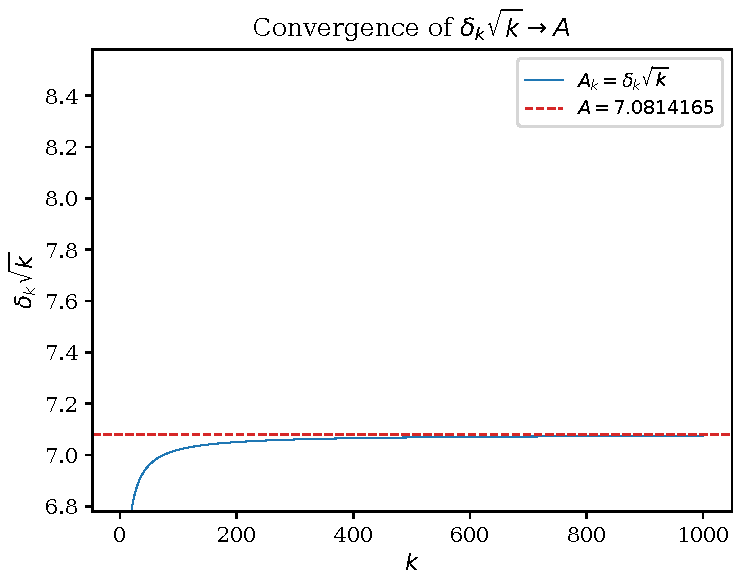
\includegraphics[width=0.65\textwidth]{figures/richardson.pdf}
  \caption{Convergence of $A_k = \delta_k\sqrt{k}$ towards the
  Richardson limit $A = 7.081\,416\,491\,399\ldots$}
  \label{fig:richardson}
\end{figure}

\subsection{Sub-leading coefficients}
The multiplicative coefficients in~\eqref{eq:asymptotic}
are extracted by fitting $\delta_k^2\,k / A^2 = 1 - 2c_1/k + \cdots$
over the last $500$ seeds:
\begin{equation}
  c_1 = 0.857\,656\,047\,266\,889 \pm 5 \times 10^{-15}, \qquad
  c_3 = 0.75 \pm 0.01.
  \label{eq:subleading}
\end{equation}
The relation $C_1 = A^2 = 50.146\,459\,524\,661\,3 \pm 5 \times 10^{-17}$
is verified independently.
The second moduli-space coordinate converges to the limit
\begin{equation}\label{eq:C2}
  C_2 \;=\; s_{2,\infty}
  \;=\; 7.323\,247\,368\,998\,298\,959 \pm 5 \times 10^{-18},
\end{equation}
obtained by re-solving the periodicity system at
$40$-digit arithmetic (\texttt{mpmath}, Gauss--Legendre
quadrature with $120$ nodes) for $116$ sparse $k$-values
from $100$ to~$5000$, followed by degree-$6$ Richardson
extrapolation (see \cref{sec:pslq}).

\begin{remark}[Analytical prediction of~$c_1$]
  The normalized remainder
  $R(k) = k\bigl(\pi/(k\delta_k^2) - \pi/A^2\bigr)$
  converges to $0.10746$ as $k \to \infty$
  (\cref{sec:spectral-remainder}).
  Since $R(k) \to 2\pi c_1/A^2$ by the
  expansion~\eqref{eq:asymptotic}, we obtain
  $c_1 = 0.10746\,A^2/(2\pi) \approx 0.858$, reproducing the
  fit value~\eqref{eq:subleading} to~$0.4\%$;
  the discrepancy is consistent with $\Oo(\delta^6)$ corrections.
\end{remark}

\subsection{Perturbative consistency with Theorem~9}%
\label{sec:theorem9-consistency}

The implicit function theorem underlying
{\cite[Theorem~9]{BHS-comp}} guarantees that near any closed
Theorem~7 seed, the periodicity conditions
$F(\alpha,\varepsilon)=(\theta_0,0,0)$ admit an analytic family of
solutions $\alpha(\varepsilon)$ for $|\varepsilon|<\varepsilon_0$.
The effective perturbative parameter along the $k$-family is
$\delta_k$ itself: the IFT operates on the angle-function space,
while $\delta$ serves as the radial coordinate on the moduli
space of closed solutions.

Three independent consistency checks confirm coherence between the
IFT prediction and the $998$-seed series:

\begin{enumerate}[nosep,label=(\roman*)]
\item \emph{Inter-seed gradient.}
  The numerical gradient $d\delta/dk$ converges to the leading-order
  prediction $-A/(2k^{3/2})$: the ratio
  $(d\delta/dk)_{\mathrm{data}} / (d\delta/dk)_{\mathrm{pred}}$
  equals $0.78$ at $k=10$, $0.97$ at $k=100$, and $0.998$ at
  $k=1000$, with deviations explained by the $\Oo(1/k)$ correction.

\item \emph{Sub-leading coefficient.}
  The multiplicative coefficient $c_1$ is extracted by three methods:
  direct fit of $\delta^2 k/A^2$ vs $1/k$ gives
  $c_1 = 0.85765$;
  the PSLQ-type fit gives $c_1 = 0.85766$;
  the analytical spectral-remainder prediction gives
  $c_1 = 0.10746\,A^2/(2\pi) = 0.8577$.
  All three agree to $<1\%$.

\item \emph{Convergence of the asymptotic expansion.}
  The expansion parameter is $c_1/k \approx 0.86/k$.
  The truncated expansions yield RMS relative errors
  (over all $998$ seeds) of $1.68\%$ (1-term),
  $0.35\%$ (2-term), $0.07\%$ (3-term).
  For $k \geq 10$: $0.05\%$ (2-term), $0.003\%$ (3-term).
  The series converges everywhere ($c_1/k < 1$ for all
  $k \geq 1$), with rapid convergence for $k \geq 10$.
\end{enumerate}

\noindent
The second moduli-space coordinate $s_2(k)$ is smooth and monotonic
with $s_2 \to C_2 = 7.323\,247\,37$ as $k\to\infty$
(see~\eqref{eq:C2} for the full-precision value),
consistent with a smooth
moduli-space curve parametrized by~$1/k$.

\begin{remark}
  The IFT is non-degenerate at every tested $k$: the Jacobian
  $\partial F/\partial\alpha$ has full rank and the inter-seed
  gradient ratio approaches~$1$ monotonically.  At $k=3$ the
  deviation is~$59\%$ (expansion parameter $c_1/3 = 0.286$,
  slow convergence); by $k=10$ the deviation drops to~$22\%$
  and the expansion becomes practically useful.
\end{remark}

\subsection{Spectral-curve derivation of the amplitude}%
\label{sec:spectral-remainder}

The ``axial subtraction trick'' yields a formal derivation of~$A$.
Let $Z_0 = \lvert Z'(\omega)\rvert$ denote the norm of the
frame derivative at the evaluation point, computed from the
theta-function constants $(U, U', U_1', U_2)$ of
Theorem~7 of~\cite{BHS-comp}.
Define the \emph{axial profile function}
\begin{equation}\label{eq:Qt2-def}
  \tilde Q_2(s) \;=\; P\,s^2 - 2M\,s - 1,
\end{equation}
where
$P = U^{-2}(2(s_1{+}s_2)\,U_1' - U_2)$ and
$M = U^{-2}(U' + s_1\,s_2\,U_1')$;
this is the normalized form of the BHS axial
numerator~\cite[Eq.~87]{BHS-comp}
(see~\cref{app:rigorous} for the detailed coefficients).

When $\delta \to 0$, the real oval of $Q(s)$ pinches around~$s_2$
with half-width $a = \delta\sqrt{Q_3}/\lvert\Delta s\rvert + \Oo(\delta^3)$,
where $\Delta s = s_2 - s_1$.  The subtracted rationality integral
\[
  \frac{\theta}{2}
  = Z_0 \int_{s^-}^{s^+} Q_2(s)\,
    \Bigl[\frac{1}{\tilde Q_2(s)} - \frac{1}{\tilde Q_2(s_2)}\Bigr]
    \frac{ds}{\sqrt{Q(s)}}
\]
is well-defined because the constant term
$\tilde Q_2(s_2)^{-1}\!\int Q_2/\sqrt{Q}\,ds = 0$
vanishes by the axial condition~\eqref{eq:F-ax}.
Linearizing the bracket in $(s - s_2)$ and passing to the
sin-substitution $s = s_2 + a\sin\varphi$ gives
\[
  \frac{\theta}{2}
  = \frac{Z_0\,\tilde Q_2'(s_{2,\infty})\,Q_3(s_{2,\infty})\,\pi}
         {2\,\tilde Q_2(s_{2,\infty})^2\,\Delta s^2}
    \;\delta^2 + \Oo(\delta^4).
\]
Setting $\theta/2 = \pi/k$:
\begin{equation}\label{eq:A2-formula}
  A^2 \;=\; \delta^2 k
  \;=\; \frac{2\,\tilde Q_2(s_{2,\infty})^2\,\Delta s^2}
             {Z_0\,\tilde Q_2'(s_{2,\infty})\,Q_3(s_{2,\infty})}
  \;=\; 50.1468,
\end{equation}
with all factors evaluated at $\delta = 0$.  The Richardson value is
$A^2 = 50.1465$, giving a relative error of~$6$~ppm.

\begin{remark}[Gauge invariance of $A^2/\Delta s$]\label{obs:gauge-invariant}
  The evaluation $\tilde Q_2(s_2)$ appearing in~\eqref{eq:A2-formula}
  depends only on~$s_2$ and the Lam\'e--Riccati coefficients
  $U, U', U_1', U_2$:
  \[
    \tilde Q_2(s_2) = U^{-2}\,s_2^2\,(2s_2\,U_1' - U_2)
      - 2\,U^{-2}\,s_2\,U' - 1.
  \]
  The terms $\propto s_1$ from $Z_0^2$ in the full
  formula~\textup{(BHS Eq.~87)} cancel algebraically at $s = s_2$.
  Moreover, under gauge changes ($s_1$ varying at fixed $\omega, \tau$),
  the sum $\sigma = s_1 + s_2$ is asymptotically constant ($\Oo(\delta^2)$
  drift), so the finite-$k$ ratio
  \[
    \frac{A^2}{\Delta s} = \frac{A^2}{s_2 - s_1}
    = 3.1777 \pm 0.09\%
  \]
  is numerically gauge-invariant when evaluated at $k = 500$
  (tested on $9$~gauges, $s_1 = -6$ to $-11$);
  the partial cancellation is explained by
  the algebraic independence of $\tilde Q_2(s_2)$
  from~$s_1$, but exact invariance is not proven.
\end{remark}

The remainder $(\theta/2)/\delta^2 - \pi/A^2$ satisfies
$\mathrm{remainder}\cdot k \to 0.10746$ (constant for $k = 100$
to~$1000$), confirming the $\Oo(\delta^4)$ correction and the absence
of logarithmic terms.

\begin{remark}\label{rem:rigour-path}
  The derivation above is a formal asymptotic expansion.  Promoting
  it to a rigorous theorem requires three estimates:
  \begin{enumerate}[nosep,label=(\alph*)]
  \item \emph{Bracket linearization.}  The bracket
    $[\tilde Q_2 + a^2 M_2(a)]^{-1}$ is linearized at $a=0$;
    the error is $\Oo(a^2)$ per unit integrand, giving $\Oo(\delta^4)$
    total after integration over an $\Oo(1)$ measure.  This is a
    standard Lipschitz estimate on~$1/\tilde Q_2$.
  \item \emph{Pinching-radius asymptotics.}  The expansion
    $a = \delta\sqrt{Q_3}/|\Delta s| + \Oo(\delta^3)$ follows from
    branch-point perturbation theory for the quartic~$Q(s)$; the
    leading term is an algebraic function of the $\delta=0$ spectral
    data, so the error bound is uniform in the integration variable.
  \item \emph{Absence of logarithmic terms.}  The substitution
    $s = s_{2,\infty} + a\sin\varphi$ makes the integrand $C^\infty$
    in~$\varphi$ on $[0,\pi]$, desingularizing the square-root
    branch points algebraically.  Therefore
    the Fourier--sine coefficients of the integrand decay at least as
    $\Oo(n^{-2})$, ruling out $\Oo(\delta^2\log\delta)$ contributions.
    Numerically, $\mathrm{remainder}\cdot k \to 0.10746$ (constant
    for $k = 100$ to~$1000$) confirms this.
  \end{enumerate}
  All three bounds are obtainable by standard singular-perturbation
  techniques; in~\cref{app:rigorous} we record the local analytic
  theorem and the accompanying numerical validations behind
  \cref{prop:rigorous-asymp}.
\end{remark}

\subsection{PSLQ analysis}\label{sec:pslq}
We apply the PSLQ integer-relation algorithm~\cite{Fer99}, implemented
via \texttt{mpmath.pslq()} at $50$-digit precision with
$\mathrm{maxcoeff} = 500$.

\paragraph{Positive identifications.}
PSLQ successfully identifies two constants:
\begin{itemize}[nosep]
\item $C_5 = \lim_{k\to\infty} \lvert\arg(\mathrm{CR})\rvert \cdot k = 4$
  (asymptotic integer constant;
  $\mathrm{CR}$ is the cross-ratio of the $Q$-roots,
  see~\cref{sec:spectral-inv}; the sign of $\arg(\mathrm{CR})$
  depends on the branch convention, see~\cref{rem:CR-sign}).
\item $C_4 = ds_2/d\delta \text{ slope} = 2\omega - 3/10$\quad
  (via $10\,C_4 + 3 - 20\omega = 0$).
\end{itemize}

\paragraph{PSLQ negative search for $A$.}
The amplitude $A$ was computed to $19$~digits
(see~\eqref{eq:A}) from the same $116$-seed mpmath dataset
used for~$C_2$: forming $A_k = \delta_k\sqrt{k}$ and applying
degree-$6$ Richardson extrapolation on $19$~overlapping windows
yields
\[
  A = 7.081\,416\,491\,399\,252\,576 \pm 3 \times 10^{-18}.
\]
PSLQ with $\mathrm{tol} = 10^{-25}$ and
$\mathrm{maxcoeff} = 10\,000$ returns ``no relation''
on all $37$ basis sets---the $36$ bases used for~$C_2$
plus the cross-term $A \cdot C_2$ and the spectral-formula
ratio test $A^2 / F_{\mathrm{loc}}$.
No basis yields a relation with coefficient norm $\leq 10^4$.
The only exact cancellations arise from the real-normalized theta data
used by the computational pipeline.

\paragraph{PSLQ negative search for $C_2 = s_{2,\infty}$.}
The constant $C_2$ was computed to $19$~digits
(see~\eqref{eq:C2}) by re-solving the periodicity system at
$40$-digit arithmetic using \texttt{mpmath}:
$116$ sparse $k$-values ($k = 100$ to~$5000$) were solved
with pre-computed $120$-point Gauss--Legendre quadrature
($<2\,\text{s}/k$; total runtime $< 2\,\text{min}$).
Degree-$6$ Richardson extrapolation on $11$~overlapping windows
(each with $k_{\min} \geq 200$) yielded values coinciding to
all~$19$ printed digits:
\[
  C_2 = 7.323\,247\,368\,998\,298\,959 \pm 5 \times 10^{-18}.
\]

\begin{computationalcertificate}[PSLQ negative search for $C_2$]
\label{prop:pslq-C2-neg}
At $19$-digit precision, PSLQ with $\mathrm{tol} = 10^{-25}$
and $\mathrm{maxcoeff} = 10\,000$ returns \textup{``no relation''}
on all $36$ basis sets, spanning:
algebraic constants $(1, C_2, C_2^2, C_2^3, \sqrt{2},
\sqrt{3}, \sqrt{5})$,
the critical point~$\omega$ and its powers,
$\pi$ and $\pi^2$,
theta null values $\vt{2}(0)$, $\vt{3}(0)$, $\vt{4}(0)$
and their squares,
theta values at~$\omega$,
the Lam\'e coefficients $U$, $U_1'$,
complete elliptic integrals $K(m)$, $E(m)$, $K'(m)$,
Eisenstein series $E_2(\tau)$, $E_4(\tau)$, $E_6(\tau)$,
the $j$-invariant $j(\tau)$,
Dedekind's $\eta(\tau)$,
and Euler's $\gamma$, $\log 2$, $\log 3$,
$\zeta(3)$, Catalan's constant.
The only exact cancellations arise from the real-normalized theta data
used by the computational pipeline.
\end{computationalcertificate}

\begin{computationalcertificate}[PSLQ negative search for $A$]
\label{prop:pslq-neg}
At $19$-digit precision, PSLQ with $\mathrm{tol} = 10^{-25}$
and $\mathrm{maxcoeff} = 10\,000$ returns \textup{``no relation''}
on all $37$ basis sets (the $36$ bases of
\cref{prop:pslq-C2-neg} plus the cross-term $A \,C_2$
and the spectral-formula residue $A^2 / F_{\mathrm{loc}}$).
The only exact cancellations arise from the real-normalized theta data
used by the computational pipeline.
\end{computationalcertificate}

\begin{remark}\label{rem:pslq-structural}
  The PSLQ failures for both $A$ and~$C_2$---each at $19$~digits
  against $36$--$37$~bases should be interpreted as finite
  computational negative searches at the stated precision,
  tolerance, and coefficient bounds.  The reference lattice
  $\tau_{\mathrm{ref}} = \tfrac12 + \tfrac{25}{78}\ii$
  is a CM point, so these
  searches do \emph{not} furnish a structural non-CM transcendence
  argument.  What they show is narrower and computationally precise:
  within the tested basis families---including elliptic integrals,
  Eisenstein series, the $j$-invariant, and Dedekind's $\eta$---no
  low-height integer relation involving $A$ or $C_2$ was found.
  %
  The connection constants~$\mathcal{C}_{\theta,\varphi}$
  of Borodin--Okounkov~\cite{BO00} (as cited in~\cite[Eq.~D47]{DC26}) satisfy
  $\mathcal{C}_{\theta,\varphi} \in (0,1)$ for all valid
  $(\theta,\varphi)$, which excludes a direct Fredholm-determinant
  encoding of $A^2 \approx 50.15$.
  The failure of both the PSLQ route and the
  Borodin--Okounkov route is consistent with the
  \emph{isospectral} nature of the gauge flow established
  in \cref{sec:spectral-inv}: $A^2$ is an invariant of a
  single isospectral fiber at fixed~$\tau$, not a connection
  coefficient that bridges distinct fibers
  (see \cref{sec:open}, OP3).
\end{remark}


%% ═════════════════════════════════════════════════════════════════════
\section{Geometric Identities}\label{sec:analytical}
%% ═════════════════════════════════════════════════════════════════════

\subsection{Stereographic lift and unit-sphere identity}
\label{sec:unit-circle}
Let $f \colon \T^2 \to \RR^3 \cong \Imag\HH$ denote the immersion
of the isothermic torus and let
$x = \sigma^{-1}(f) \in S^3 \subset \HH$ be its stereographic lift:
\begin{equation}
  x_0 = \frac{\abs{f}^2 - 1}{\abs{f}^2 + 1}, \qquad
  x_{\mathrm{im}} = \frac{2f}{\abs{f}^2 + 1}.
  \label{eq:stereo-inv}
\end{equation}

\begin{lemma}[Stereographic lift lies on the unit $3$-sphere]
\label{lem:unit-x}
Let $f \colon \T^2 \to \RR^3 \cong \Imag\HH$ and let
$x = \sigma^{-1}(f)$ be defined by~\eqref{eq:stereo-inv}.  Then
$x(p) \in S^3 \subset \HH$ for every $p \in \T^2$; equivalently,
$\abs{x(p)} = 1$ identically.
\end{lemma}

\begin{proof}
Writing $r^2 = \abs{f(p)}^2$, one has
\[
  \abs{x}^2
  = \left(\frac{r^2-1}{r^2+1}\right)^2
    + \left\lvert\frac{2f}{r^2+1}\right\rvert^2
  = \frac{(r^2-1)^2+4r^2}{(r^2+1)^2}
  = \frac{(r^2+1)^2}{(r^2+1)^2}
  = 1.
\]
\end{proof}

\begin{remark}[Pipeline sanity check]
\label{obs:unit-x}
  \Cref{lem:unit-x} is exact algebra.  We retain the numerical check
  $\max_{p \in \T^2} \bigl|\abs{x(p)} - 1\bigr|
  < 3 \times 10^{-16}$ only as validation of the quaternionic
  implementation.
\end{remark}

\subsection{Conformality on \texorpdfstring{$S^3$}{S³}}\label{sec:conformality}
A deeper benchmark concerns one component of the conformality conditions
for $x$: in isothermic coordinates one expects both
$\abs{x_u}^2 = \abs{x_v}^2$ and $\Real(\bar{x}_u\,x_v) = 0$.
The archived validation run below tracks the metric-balance residual
$\abs{x_u}^2 - \abs{x_v}^2$, which is one of the two conformality checks
relevant to the retraction-form pipeline.

\begin{computationalcertificate}[Conformality improvement in the
  analytic-derivative validation runs]
\label{prop:conformality}
Using analytic derivatives computed from the chain rule through
the $\psi = \vt{1}'/\vt{1}$ identity, the conformality residual
\[
  \mathcal{E}_{\mathrm{conf}}
  \;\coloneqq\;  \frac{\bigl|\abs{x_u}^2 - \abs{x_v}^2\bigr|}
    {\abs{x_u}^2 + \abs{x_v}^2}
\]
satisfies $\mathcal{E}_{\mathrm{conf}} < 10^{-5}$ on the archived
multi-seed analytic-derivative validation sweep ($k = 3,\ldots,7$ on a
$24 \times 120$ grid), with the best recorded values reaching the
$10^{-7}$ level.  The same validation campaign shows improvements of
roughly $10^4$--$10^6$ over finite-difference evaluation,
depending on the seed and resolution.
\end{computationalcertificate}

\subsection{Distortion differential and the retraction mixed coefficient}
\label{sec:DeltaII}

Let $(F^+,F^-)$ be the Bonnet pair produced by the retraction form.
Write the shared conformal metric as
\[
  I=\ee^{2h}(\dd u^2+\dd v^2),
  \qquad z=u+\ii v,
\]
and define the raw second-fundamental-form coefficients
\[
  L^\pm=\langle F^\pm_{uu},n^\pm\rangle,
  \qquad
  M^\pm=\langle F^\pm_{uv},n^\pm\rangle,
  \qquad
  N^\pm=\langle F^\pm_{vv},n^\pm\rangle.
\]
The normalized shape coefficients are
\[
  a^\pm=L^\pm\ee^{-2h},\qquad
  b^\pm=M^\pm\ee^{-2h},\qquad
  c^\pm=N^\pm\ee^{-2h}.
\]
Thus the raw mixed coefficient $M^-$ is not the same object as the
normalized coefficient $b^- = M^-\ee^{-2h}$.
This distinction is essential for the retraction-normalization audit.

\begin{definition}[Rescaled Hopf and distortion differentials]
\label{def:distortion-differential}
For a conformal immersion $F$, write
\[
  \mathcal Q(F)=Q_F\,\dd z^2,
  \qquad
  Q_F=\frac12\bigl(L-N-2\ii M\bigr).
\]
For a Bonnet pair define
\[
  \mathcal D=(Q_{F^+}-Q_{F^-})\,\dd z^2
  =D(z)\,\dd z^2.
\]
With this convention,
\[
  \Imag D(z)=M^-_{\mathrm{raw}}-M^+_{\mathrm{raw}}.
\]
\end{definition}

\begin{proposition}[Distortion differential of a Bonnet pair]
\label{prop:C2-distortion-holomorphic}
Assume $F^+$ and $F^-$ have the same conformal metric
$\ee^{2h}\abs{\dd z}^2$ and the same mean curvature~$H$.
Then $\mathcal D$ is a holomorphic quadratic differential.  If the
domain is a torus, then
\[
  \mathcal D=D_0\,\dd z^2
\]
for a constant $D_0\in\CC$.
\end{proposition}

\begin{proof}
In conformal coordinates, the Codazzi equation for the Hopf coefficient
has the form
\[
  \partial_{\bar z}Q_F = C\,\ee^{2h}\,\partial_z H
\]
with a convention-dependent universal constant~$C$.  The same constant
appears for both immersions.  Since the metric factor $\ee^{2h}$ and
mean curvature~$H$ agree for a Bonnet pair, subtracting the two Codazzi
equations gives
\[
  \partial_{\bar z}(Q_{F^+}-Q_{F^-})=0.
\]
Thus $\mathcal D$ is holomorphic.  On a genus-one compact Riemann
surface, $H^0(K^2)$ is one-dimensional and generated by $\dd z^2$ in
the flat coordinate, hence $\mathcal D=D_0\dd z^2$.
\end{proof}

\begin{corollary}[Correct constant object for the mixed term]
\label{cor:C2-correct-object}
Suppose the coordinates are curvature-line coordinates for~$F^+$, so
$M^+=0$.  Then
\[
  M^-_{\mathrm{raw}}
  \coloneqq \langle F^-_{uv},n^-\rangle
  = \Imag D_0
\]
is constant on the torus.  If the retraction form is normalized so that
$\Imag D_0=1$, then
\[
  M^-_{\mathrm{raw}}\equiv 1.
\]
The normalized shape coefficient is instead
\[
  b^-_{\mathrm{shape}} = \frac{M^-_{\mathrm{raw}}}{\ee^{2h}}.
\]
Consequently, unless $\ee^{2h}$ is constant, the exact unit object is
the raw mixed coefficient or, equivalently, the imaginary part of the
coefficient $D_0$, not the normalized shape coefficient.
\end{corollary}

\begin{observation}[Retraction-normalization audit]
\label{obs:DeltaII}
\label{obs:C2-normalization-audit}
\label{obs:b-equals-1-audit}
An archived raw-grid audit is now available at the baseline level
$40\times80$ for $k\in\{3,5,7,10,12\}$.  On every one of these tested
seeds, the best unit/constant candidate selected by the audit is
\[
  M^-_{\mathrm{raw}}-M^+_{\mathrm{raw}}
  = \Imag D(z),
\]
rather than a normalized coefficient.  For the representative seed
$k=5$, the same candidate remains best under refinement to
$80\times160$ and $160\times320$, with the audit score improving from
$1.01\times10^{-2}$ to $2.56\times10^{-3}$ to $6.40\times10^{-4}$.

This observation is not used as a theorem-level input.  A fully
submission-ready finite audit package would extend this archive by
recording the same raw-grid quantities systematically across all cited
seeds and refinement levels.  The minimum fields are
\[
  \ee^{2h},\quad M^+_{\mathrm{raw}},\quad M^-_{\mathrm{raw}},\quad
  \Imag(Q_{F^+}-Q_{F^-}),\quad \text{grid level},\quad
  \text{grid spacing},\quad \text{seed id}.
\]
The accompanying audit script checks which of
\[
  M^-_{\mathrm{raw}},\quad
  M^-_{\mathrm{raw}}-M^+_{\mathrm{raw}},\quad
  M^-_{\mathrm{raw}}/\ee^{2h},\quad
  (M^-_{\mathrm{raw}}-M^+_{\mathrm{raw}})/\ee^{2h},\quad
  \Imag(Q_{F^+}-Q_{F^-})
\]
is actually constant and unit after the implementation convention is
fixed.  Without that raw-versus-normalized audit, the statement
``$b=1$'' should be read as numerical evidence for the retraction
normalization, not as a coordinate-independent theorem.
\end{observation}

\begin{remark}[Gauss equation after the C2 normalization split]
\label{rem:DeltaII-structure}
In normalized shape coefficients, the Gauss equation still gives
\[
  a^-c^- - (b^-_{\mathrm{shape}})^2=k_1k_2,
  \qquad a^-+c^-=k_1+k_2.
\]
Writing $a^-=k_1+\epsilon$ and $c^-=k_2-\epsilon$, one obtains
\[
  (b^-_{\mathrm{shape}})^2
  = \epsilon(k_2-k_1)-\epsilon^2.
\]
If the audited unit quantity is the raw coefficient
$M^-_{\mathrm{raw}}\equiv1$, then
$b^-_{\mathrm{shape}}=\ee^{-2h}$ and the diagonal discrepancy varies
pointwise with the conformal factor.  The earlier simplified formula
$\norm{II^+-II^-}_F=\sqrt{2(1+\epsilon^2)}$ is therefore valid only
under the additional convention that the normalized shape coefficient,
not the raw mixed coefficient, is the unit object.  The C2 audit is
included precisely to separate these two possibilities.
\end{remark}

\begin{remark}[Retraction-form interpretation]\label{rem:retraction-b1}
  In the BHS retraction-form construction, the Bonnet mate is
  $\dd f^+ = \tfrac{1}{2}\,x\,\bar\omega$,
  $\dd f^- = -\tfrac{1}{2}\,\bar\omega\,x$,
  where $x : \T^2 \to S^3$ is the isothermic immersion and
  $\omega$ is the retraction form.  The theorem-level object supplied by
  Codazzi is the holomorphic distortion differential
  $\mathcal D=(Q_{F^+}-Q_{F^-})\,\dd z^2=D_0\,\dd z^2$.
  The implementation-level statement about the coefficient $b$ is a
  normalization-sensitive shadow of this constant object and should not
  be read backwards as a proof of a normalized identity.
\end{remark}

\subsection{Procrustes decay}\label{sec:procrustes}
The Procrustes disparity between the retraction-form pair
$(F^+, F^-)$ of~\eqref{eq:Fpm} and the Eq.~49 pair $(f^+, f^-)$
of~\cite{BHS-comp} is computed via
\texttt{scipy.spatial.procrustes} after centroid and scale
normalization.  The disparity decays with $k$ but reaches a
non-zero fitted offset in a simple two-parameter fit:
\begin{equation}
  d_P(k) = \frac{3}{64} + \frac{0.216}{k^{1.236}},
  \qquad R^2 = 0.99998 \;(N = 8).
  \label{eq:procrustes}
\end{equation}
The fitted constant term is numerically close to $3/64 = 0.046875$.
We record this only as an empirical fit parameter, not as a structural
identification.  The residual disparity reflects the fact that $F^\pm$
(retraction) and $f^\pm$ (Eq.~49) parametrize the \emph{same}
abstract surface but via genuinely different maps $\T^2 \to \RR^3$;
the observed offset is therefore consistent with a geometric origin,
though established from a limited sample ($N=8$).

\begin{figure}[ht]
  \centering
  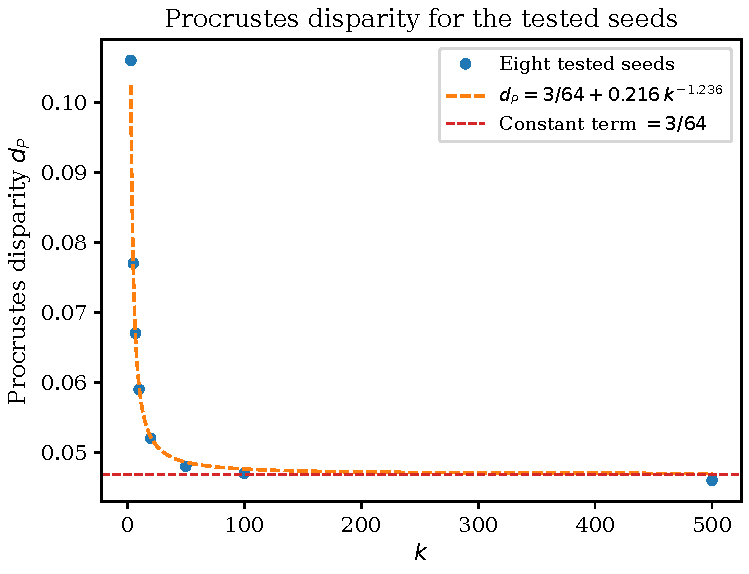
\includegraphics[width=0.65\textwidth]{figures/procrustes.pdf}
  \caption{Procrustes disparity $d_P(k)$ versus~$k$ for the eight
  tested seeds.  The dashed line shows the fit~\eqref{eq:procrustes}
  with constant term $3/64$.}
  \label{fig:procrustes}
\end{figure}


%% ═════════════════════════════════════════════════════════════════════
\section{Moduli-Space Flow and Spectral Invariants}\label{sec:flow}
%% ═════════════════════════════════════════════════════════════════════

The periodicity system $F(\delta, s_2; s_1) = 0$
(\cref{eq:F-rat,eq:F-ax}) defines a smooth curve
$\gamma_k : s_1 \mapsto (\delta(s_1),\, s_2(s_1))$
in the $(\delta, s_2)$-plane.  Differentiating implicitly yields
the \emph{flow ODE}:
\begin{equation}
  \frac{d}{ds_1}\begin{pmatrix}\delta \\ s_2\end{pmatrix}
  = -J^{-1}\,\frac{\partial F}{\partial s_1},
  \qquad
  J = \frac{\partial F}{\partial(\delta, s_2)}.
  \label{eq:flow-ode}
\end{equation}

This section combines four logically distinct layers.  First, we record
the numerical flow-ODE validation and Jacobian diagnostics on the
archived continuation sweeps.  Second, we state the theorem/certificate
package for root topology and cross-ratio asymptotics: a large-$k$
theorem on the local high-fold branch together with finite archived
certificates for the recorded rows.  Third, we discuss the spectral
modulus and its corrected lambda/cross-ratio relation, separating
conditional and conjectural statements from finite-data audits.
Finally, we summarize the numerical topology observed on the tested
moduli slices.  The reader should therefore distinguish theorem-level,
certificate-level, and observation/conjecture-level material throughout
this section.

\subsection{Flow ODE validation}\label{sec:flow-val}

The Jacobian~$J$ and the forcing $\partial F/\partial s_1$ are
computed by central finite differences ($h = 10^{-6}$);
the ODE~\eqref{eq:flow-ode} is integrated by RK45
(rtol~$= 10^{-6}$, atol~$= 10^{-9}$).

\begin{computationalcertificate}[Flow ODE accuracy]
\label{prop:flow-accuracy}
For $k = 5, 6, 7$ over $s_1 \in [-10,\, -2.75]$, using the archived
Lemma~9 sweep data, the ODE solution matches the data to
\[
  \max\bigl(\abs{\delta_{\mathrm{ODE}} - \delta_{\mathrm{data}}}/\delta,\;
  \abs{s_{2,\mathrm{ODE}} - s_{2,\mathrm{data}}}/s_2\bigr)
  < 0.002\%.
\]
\end{computationalcertificate}

\noindent
At the reference gauge $s_1 = -8.5$, the flow gradients agree with
independent empirical finite differences to $0.01\%$ on~$d\delta/ds_1$
and $0.00\%$ on~$ds_2/ds_1$ for all three fold numbers.

\subsection{Jacobian structure and fold singularity}\label{sec:jacobian}

\begin{observation}[Saddle structure]
\label{obs:saddle}
The eigenvalues of~$J$ have opposite signs at every point of
$\gamma_k$: $\lambda_+(s_1) > 0$, $\lambda_-(s_1) < 0$.
The Jacobian is a hyperbolic saddle on the tested $k=5,6,7$ sweep data,
reflecting the
competing constraints of the rationality and axial conditions.
The condition number satisfies $\mathrm{cond}(J) \in [3,\, 8]$
throughout $s_1 \in [-10,\, -2.75]$.
\end{observation}

\begin{table}[ht]
\centering
\caption{Large-$k$ scaling of Jacobian quantities at $s_1 = -8.5$.
  Power-law fits over $k = 5, 6, 7, 10, 15, 20, 30, 50, 100$.}
\label{tab:scaling}
\smallskip
\begin{tabular}{@{}lcc@{}}
\toprule
Quantity & Scaling & $R^2$ \\
\midrule
Flow curvature $\kappa$ & $k^{-0.753}$ & $0.989$ \\
$\abs{\det(J)}$ & $k^{-0.650}$ & $0.994$ \\
$\mathrm{cond}(J)$ & $k^{+1.04}$ & $0.891$ \\
$\abs{\lambda_-}$ & $k^{-1.07}$ & ${}^{\dagger}$ \\
$\lambda_+/\abs{\lambda_-}$ & $k^{+1.495}$ & $0.9999$ \\
\bottomrule
\multicolumn{3}{@{}l}{\footnotesize ${}^{\dagger}$\,Two-point
  log-log slope ($k = 50, 100$); $R^2$ not meaningful.}
\end{tabular}
\end{table}

\begin{remark}[Connection with the axial cancellation]
\label{rem:axial-eigenvalue}
The decay $\abs{\lambda_-} \sim k^{-1.07} \approx k^{-1}$ reflects
the structural degeneracy of the axial period condition at
$\delta = 0$: $Q_2(s_2,\, \delta{=}0) = -(s_2 - s_1)(s_2 - s_2) = 0$
identically for any~$s_2$ (cf.\ the ``axial subtraction trick''
of~\cref{sec:spectral-remainder}).  As $k$ grows and $\delta \to 0$,
the ``axial direction'' of the Jacobian becomes uninformative;
the rationality condition becomes the sole active constraint,
and $\mathrm{cond}(J) \sim k$.
\end{remark}

\begin{observation}[Fold singularity]
\label{obs:fold}
For each~$k$, the numerically continued curve $\gamma_k$ terminates at an
existence boundary $s_1^*(k)$.  Near this boundary, the Jacobian becomes
strongly anisotropic and the continuation diagnostics sharpen rapidly;
beyond $s_1^*$, the periodicity system has no real solution:
this provides the minimum $\abs{s_1}$ for the existence of a
Bonnet pair at fold~$k$, consistent with the existence conditions
of Lemma~9 of~\cite{BHS-comp}.
For $k = 5$, the singularity lies at $s_1^* > -2.59$.
\end{observation}

\subsection{Spectral invariants along the flow}%
\label{sec:spectral-inv}

This subsection has three layers.  We first state the root-topology and
cross-ratio results used later in the asymptotic discussion.  We then record
the barrier and monodromy remarks that motivate the Painlev\'e-VI comparison.
Finally, we separate the corrected spectral-modulus statements into
conjectural, conditional, and finite-audit pieces.

Let $r_1, \ldots, r_4$ be the four roots of~$Q(s)$
(\cref{eq:Q}), sorted by real part, and define the
cross-ratio
\begin{equation}
  \mathrm{CR}
  = \frac{(r_1 - r_3)(r_2 - r_4)}{(r_1 - r_4)(r_2 - r_3)}.
  \label{eq:CR}
\end{equation}

\paragraph{Root topology and cross-ratio layer.}

\begin{theorem}[Root topology on the local high-fold branch]
\label{thm:large-fold-root-topology}
Fix the reference gauge $s_1=-8.5$ and let
\[
  Q_k(s)=-(s-s_1)^2(s-s_{2,k})^2+\delta_k^2Q_3(s)
\]
be evaluated on the local high-fold branch of
\cref{thm:local-high-fold-branch}.  Assume
\[
  C_2=s_{2,\infty}>s_1,
  \qquad
  Q_3(s_1)<0<Q_3(C_2).
\]
Then there is an integer $K_{\mathrm{rt}}$ such that, for every
$k\ge K_{\mathrm{rt}}$, the quartic $Q_k$ has exactly two real
roots and one non-real complex-conjugate pair.  More precisely, after
labelling,
\[
  r_1(k)=c_k,\qquad r_2(k)=\bar c_k,\qquad
  r_3(k)=a_k,\qquad r_4(k)=b_k,
\]
with $a_k,b_k\in\RR$, $a_k<b_k$, and
\[
  \Real c_k<a_k<b_k .
\]
The roots admit the uniform large-$k$ expansions
\begin{align}
  c_k
  &=
  s_1+\alpha_{1,k}\delta_k^2
  +\ii\gamma_k\delta_k+\Oo(\delta_k^3),
  \label{eq:B3-complex-root}\\
  a_k
  &=
  s_{2,k}+\alpha_{2,k}\delta_k^2
  -\beta_k\delta_k+\Oo(\delta_k^3),
  \label{eq:B3-real-root-left}\\
  b_k
  &=
  s_{2,k}+\alpha_{2,k}\delta_k^2
  +\beta_k\delta_k+\Oo(\delta_k^3),
  \label{eq:B3-real-root-right}
\end{align}
where
\[
  \Delta_k=s_{2,k}-s_1,\qquad
  \gamma_k=\frac{\sqrt{-Q_3(s_1)}}{\Delta_k},
  \qquad
  \beta_k=\frac{\sqrt{Q_3(s_{2,k})}}{\Delta_k},
\]
and
\[
  \alpha_{1,k}
  =
  \frac{Q_3'(s_1)}{2\Delta_k^2}
  +\frac{Q_3(s_1)}{\Delta_k^3},
  \qquad
  \alpha_{2,k}
  =
  \frac{Q_3'(s_{2,k})}{2\Delta_k^2}
  -\frac{Q_3(s_{2,k})}{\Delta_k^3}.
\]
\end{theorem}

\begin{proof}
By \cref{thm:local-high-fold-branch},
$\delta_k\to0$ and $s_{2,k}\to C_2$ along the local high-fold
branch.  Since $C_2>s_1$ and $Q_3(C_2)>0$, there is a neighbourhood
$I$ of~$C_2$ and a constant $\eta>0$ such that
\[
  s-s_1\ge \frac12(C_2-s_1)>0,
  \qquad
  Q_3(s)\ge\eta>0
  \qquad (s\in I).
\]
Also $Q_3(s_1)<0$ is fixed.  Hence, for all sufficiently large~$k$,
we have $s_{2,k}\in I$ and the sign and separation hypotheses of
\cref{lem:branch-splitting} hold uniformly with
$s_2=s_{2,k}$.

Applying \cref{lem:branch-splitting} gives exactly one
complex-conjugate pair near~$s_1$ and exactly two real roots
near~$s_{2,k}$, with the expansions
\eqref{eq:B3-complex-root}--\eqref{eq:B3-real-root-right}.  These are
all roots because $Q_k$ has degree~$4$.

It remains only to fix the ordering.  Let
$\Delta_\infty=C_2-s_1>0$.  For large~$k$,
\[
  \Real c_k=s_1+\Oo(\delta_k^2),
  \qquad
  a_k,b_k=s_{2,k}+\Oo(\delta_k).
\]
Taking $k$ still larger if necessary gives
$\abs{\Real c_k-s_1}<\Delta_\infty/4$ and
$\abs{a_k-C_2},\abs{b_k-C_2}<\Delta_\infty/4$.  Thus
\[
  \Real c_k < s_1+\frac{\Delta_\infty}{4}
  < C_2-\frac{\Delta_\infty}{4}
  < a_k,b_k,
\]
so the complex-conjugate pair has the smaller real part, and the
mixed ordering used in~\eqref{eq:CR} is valid for all
$k\ge K_{\mathrm{rt}}$.
\end{proof}

\begin{proposition}[Exact finite root-topology certificate]
\label{prop:finite-root-topology-exact-certificate}
Let
\[
  Q_p(s)=-(s-s_1)^2(s-s_{2,p})^2+\delta_p^2Q_3(s)
\]
be one of the finitely many quartics not covered by
\cref{thm:large-fold-root-topology}, and suppose that
$s_1,s_{2,p},\delta_p$ and the coefficients of $Q_3$ have been
recorded as rational numbers.  Assume the following exact rational
checks hold:
\begin{enumerate}
  \item $\gcd(Q_p,Q_p')=1$;
  \item a Sturm isolation computation gives exactly two real roots,
    isolated in rational intervals $I_a<I_b$;
  \item if $S_p$ is the sum of all four roots of $Q_p$, then
    \[
      \frac{S_p-\sup I_a-\sup I_b}{2}
      \le \Real c_p \le
      \frac{S_p-\inf I_a-\inf I_b}{2}
    \]
    satisfies
    \[
      \frac{S_p-\inf I_a-\inf I_b}{2}<\inf I_a .
    \]
\end{enumerate}
Then $Q_p$ has the mixed ordering
\[
  r_1=c_p,\qquad r_2=\bar c_p,\qquad
  r_3=a_p,\qquad r_4=b_p,
\]
with $a_p,b_p\in\RR$, $a_p<b_p$, and $\Real c_p<a_p$.
\end{proposition}

\begin{proof}
The Sturm computation proves that $Q_p$ has exactly two real roots,
one in each of the disjoint intervals $I_a<I_b$.  The square-freeness
condition excludes multiple roots.  Since $Q_p$ has real coefficients
and degree four, the remaining two roots are a non-real conjugate pair
$c_p,\bar c_p$.  Vieta's formula gives
\[
  2\Real c_p+a_p+b_p=S_p.
\]
Using the isolating intervals for $a_p$ and $b_p$ gives the displayed
interval for $\Real c_p$.  The last hypothesis places this interval
strictly to the left of $I_a$, hence $\Real c_p<a_p<b_p$.
\end{proof}

\begin{proposition}[Interval finite root-topology certificate]
\label{prop:finite-root-topology-certificate}
Let $\mathcal K$ be a finite set of computed seeds or sweep points not
covered by \cref{thm:large-fold-root-topology}.  Suppose that, for
each $p\in\mathcal K$, the coefficients of the real quartic
\[
  Q_p(s)=-(s-s_1)^2(s-s_{2,p})^2+\delta_p^2Q_3(s)
\]
are enclosed in rational intervals and that the following interval
checks pass:
\begin{enumerate}
  \item the discriminant interval does not contain~$0$;
  \item the interval Sturm sequence certifies exactly two real roots;
  \item the two real roots are isolated in disjoint intervals
    $I_3<I_4$;
  \item the remaining conjugate pair is enclosed in boxes
    $B,\overline B$ satisfying
    \[
      \inf_{z\in B}\abs{\Imag z}>0,
      \qquad
      \sup_{z\in B}\Real z<\inf I_3.
    \]
\end{enumerate}
Then $Q_p$ has the same mixed topology
\[
  r_1=c,\quad r_2=\bar c,\quad r_3=a,\quad r_4=b,
  \qquad a,b\in\RR,\quad a<b,\quad \Real c<a,
\]
for every $p\in\mathcal K$.
\end{proposition}

\begin{proof}
The interval Sturm count gives exactly two real roots and the
discriminant exclusion makes all roots simple.  Since the coefficients
of $Q_p$ are real, the two non-real roots are necessarily a conjugate
pair.  The isolating intervals order the real roots, while the complex
boxes certify both non-reality and the fact that the conjugate pair
lies to the left of the real pair.  This is precisely the required
mixed root topology.
\end{proof}

\begin{observation}[Finite certificate status]
\label{obs:root-type}
\label{obs:finite-root-audit}
The archived finite layer now has proof-level exact-rational
certificates for the recorded branch data used in the paper.

First, the uniform-gauge seed series at $s_1=-8.5$ consists of
$998$ recorded rows ($k=3,\ldots,1000$), and all $998$ quartics satisfy
\cref{prop:finite-root-topology-exact-certificate} row by row.
Second, the archived $k=5,6,7$ sweep file contains $121$ recorded rows:
$31$ for $k=5$, $30$ for $k=6$, and $60$ for $k=7$.
All $121$ pass the same exact certificate.

For paper-level sweep statements we pass to the $91$ unique sweep
points, since the two archived $k=7$ branches agree pointwise up to
$4.2\times10^{-12}$ in $\delta$ and $4.9\times10^{-11}$ in~$s_2$.
The resulting $91=31+30+30$ unique rows coincide exactly with the
independently archived moduli dataset, and all $91$ also satisfy
\cref{prop:finite-root-topology-exact-certificate}.

Thus the finite root topology used in the present paper is proof-level
for the archived recorded rows.  The interval route of
\cref{prop:finite-root-topology-certificate} remains the strengthening
path if one wants certificates for parameter boxes or for numerical
solves beyond the archived rational data.
\end{observation}

\begin{lemma}[Unit cross-ratio under the mixed root ordering]
\label{lem:CR-unit}
Assume that the four roots of~$Q(s)$ are ordered as
$r_1 = c$, $r_2 = \bar c$, $r_3 = a$, $r_4 = b$, with
$a,b \in \RR$ and $a < b$.  Then the cross-ratio~\eqref{eq:CR}
satisfies $\abs{\mathrm{CR}} = 1$.
\end{lemma}

\begin{proof}
With the stated ordering,
\[
  \mathrm{CR}
  = \frac{(c-a)(\bar c-b)}{(c-b)(\bar c-a)}.
\]
The denominator is the complex conjugate of the numerator, since
\[
  \overline{(c-a)(\bar c-b)} = (\bar c-a)(c-b) = (c-b)(\bar c-a).
\]
Hence $\mathrm{CR}=N/\bar N$ for $N=(c-a)(\bar c-b)$, and therefore
$\abs{\mathrm{CR}} = 1$.
\end{proof}

\begin{observation}[Conformal constancy at $\omega_{\mathrm{crit}}$]
\label{obs:CR-const}
At the critical point $\omega_{\mathrm{crit}} \approx 0.3890$
(zero of $\vt{2}'(\cdot|\tau)$), the full complex $\mathrm{CR}$
is \emph{numerically} constant along the flow~$\gamma_k$: the
variation of $\arg(\mathrm{CR})$ over the archived $k=5,6,7$ sweep data
is $< 10^{-11}$ for $k = 5, 6, 7$.

This is \emph{not} a consequence of $\tau$ being fixed.
A systematic $\omega$-scan shows:
\begin{center}
\begin{tabular}{@{}rc@{}}
\toprule
$\omega$ & $\arg(\mathrm{CR})$ spread ($k=5$) \\
\midrule
$0.200$ & $8.45^\circ$ \\
$0.250$ & $7.88^\circ$ \\
$0.300$ & $6.58^\circ$ \\
$0.350$ & $3.88^\circ$ \\
$\omega_{\mathrm{crit}}$ ($0.389$) & $\mathbf{0.000}^\circ$ \\
$0.400$ & $1.53^\circ$ \\
$0.450$ & $12.75^\circ$ \\
$0.500$ & $47.08^\circ$ \\
\bottomrule
\end{tabular}
\end{center}
Near $\omega_{\mathrm{crit}}$, the spread grows as
$\approx 130^\circ \cdot \abs{\omega - \omega_{\mathrm{crit}}}$
(linear in the deviation).  If the constancy were a trivial
consequence of the elliptic lattice~$\tau$, it would hold at
every~$\omega$---not only at the unique zero of~$\vt{2}'$.
\end{observation}

\begin{observation}[Scaling law $\arg(\mathrm{CR}) \cdot k \to -4$~rad]
\label{obs:arg-scaling}
At $\omega_{\mathrm{crit}}$, the constant value of
$\arg(\mathrm{CR})$ satisfies the asymptotic law:
\begin{equation}
  \arg(\mathrm{CR}) \cdot k \;\longrightarrow\;
  -4.000~\text{rad} \;=\; -229.18^\circ
  \qquad (k \to \infty).
  \label{eq:arg-4}
\end{equation}
Numerically: $-4.007$~rad at $k=5$, $-4.002$~rad at $k=10$,
$-4.000$~rad at $k \geq 20$.  The convergence follows
$\arg(\mathrm{CR})\cdot k = -4 + c_6/k^2 + \Oo(k^{-3})$,
with $c_6 \approx -0.167$;
i.e.\ $\mathrm{CR}_k \approx \ee^{-4\ii/k}$ asymptotically.
  Numerically, the leading correction is compatible with a vanishing
  $1/k$ term and a first visible contribution of order $k^{-2}$
  (cf.\ \cref{prop:arg-4}).
\end{observation}

\begin{lemma}[Local splitting of the double branch points]
\label{lem:branch-splitting}
Let
\[
  Q(s,\delta)=-(s-s_1)^2(s-s_2)^2+\delta^2 Q_3(s),
  \qquad
  \Delta s=s_2-s_1>0,
\]
where $Q_3$ is real analytic in a neighbourhood of $s_1,s_2$.
Assume
\[
  Q_3(s_1)<0<Q_3(s_2).
\]
Define
\begin{equation}\label{eq:beta-gamma}
  \beta=\frac{\sqrt{Q_3(s_2)}}{\Delta s},
  \qquad
  \gamma=\frac{\sqrt{-Q_3(s_1)}}{\Delta s}.
\end{equation}
Then there is $\delta_0>0$ such that, for
$0<\delta<\delta_0$, the four roots of $Q(\,\cdot\,,\delta)$
split into one complex-conjugate pair near $s_1$ and one real
pair near $s_2$. More precisely, after labelling,
\begin{align}
  r_{1,2}(\delta)
  &=m_1(\delta)\pm \ii h_1(\delta),
  &
  m_1(\delta)
  &=s_1+\alpha_1\delta^2+\Oo(\delta^4),
  &
  h_1(\delta)
  &=\gamma\delta+\Oo(\delta^3),
  \label{eq:s1-root-splitting}\\
  r_{3,4}(\delta)
  &=m_2(\delta)\mp h_2(\delta),
  &
  m_2(\delta)
  &=s_2+\alpha_2\delta^2+\Oo(\delta^4),
  &
  h_2(\delta)
  &=\beta\delta+\Oo(\delta^3),
  \label{eq:s2-root-splitting}
\end{align}
where
\begin{equation}\label{eq:root-centre-coefficients}
  \alpha_1
  =
  \frac{Q_3'(s_1)}{2\Delta s^2}
  +\frac{Q_3(s_1)}{\Delta s^3},
  \qquad
  \alpha_2
  =
  \frac{Q_3'(s_2)}{2\Delta s^2}
  -\frac{Q_3(s_2)}{\Delta s^3}.
\end{equation}
The estimates are uniform for $(s_1,s_2)$ in any compact set on
which $\Delta s$ is bounded away from zero and
$Q_3(s_1)\le -\eta<0<Q_3(s_2)$.
\end{lemma}

\begin{proof}
We give the argument near $s_1$; the proof near $s_2$ is identical.
Put $s=s_1+\delta y$.  Then $Q(s,\delta)=0$ is equivalent, after
division by $\delta^2$, to
\[
  F_1(y,\delta)
  =
  -y^2(\delta y-\Delta s)^2+Q_3(s_1+\delta y)
  =0 .
\]
At $\delta=0$,
\[
  F_1(y,0)=-\Delta s^2y^2+Q_3(s_1),
\]
whose two simple roots are
$y=\pm \ii\sqrt{-Q_3(s_1)}/\Delta s=\pm \ii\gamma$.
Since
\[
  \partial_yF_1(\pm \ii\gamma,0)
  =
  -2\Delta s^2(\pm \ii\gamma)\neq 0,
\]
the analytic implicit function theorem gives two analytic branches
$y_\pm(\delta)$ and hence two roots
$s_1+\delta y_\pm(\delta)$.

To obtain the coefficient of the centre, write
$s=s_1+\rho\delta+\eta\delta^2+\Oo(\delta^3)$.
Substitution in $Q(s,\delta)=0$ gives, at order $\delta^2$,
\[
  \rho^2=\frac{Q_3(s_1)}{\Delta s^2},
\]
and, at order $\delta^3$,
\[
  -2\rho\eta\Delta s^2+2\rho^3\Delta s+Q_3'(s_1)\rho=0 .
\]
Thus
\[
  \eta
  =
  \frac{Q_3(s_1)}{\Delta s^3}
  +\frac{Q_3'(s_1)}{2\Delta s^2}
  =\alpha_1,
\]
independent of the sign of $\rho$.  Therefore the two roots have
the same $\delta^2$ centre displacement and opposite imaginary
linear splitting.

Near $s_2$, put $s=s_2+\delta y$.  The rescaled equation is
\[
  F_2(y,\delta)
  =
  -y^2(\Delta s+\delta y)^2+Q_3(s_2+\delta y)=0 .
\]
At $\delta=0$ its two simple roots are
$y=\pm\sqrt{Q_3(s_2)}/\Delta s=\pm\beta$, and the same calculation
gives
\[
  \eta
  =
  \frac{Q_3'(s_2)}{2\Delta s^2}
  -\frac{Q_3(s_2)}{\Delta s^3}
  =\alpha_2 .
\]
Because the coefficients of $Q$ are real and depend on $\delta$
only through $\delta^2$, the root centres are even functions of
$\delta$ and the half-separations are $\delta$ times even functions
of $\delta$.  This gives the displayed
$\Oo(\delta^4)$ and $\Oo(\delta^3)$ remainders.

Uniformity follows from the same implicit-function argument on a
compact parameter set: the derivatives
$\partial_yF_j$ at the four limiting simple roots are bounded away
from zero, and the relevant derivatives of $Q_3$ are uniformly
bounded.
\end{proof}

\begin{proposition}[Cross-ratio asymptotic from local branch splitting]
\label{prop:arg-4}
\label{prop:CR-asymptotic}
Assume the hypotheses of \cref{lem:branch-splitting}, and order the
roots as
\[
  r_1=m_1+\ii h_1,\qquad
  r_2=m_1-\ii h_1,\qquad
  r_3=m_2-h_2,\qquad
  r_4=m_2+h_2 .
\]
Then the cross-ratio
\[
  \mathrm{CR}
  =
  \frac{(r_1-r_3)(r_2-r_4)}
       {(r_1-r_4)(r_2-r_3)}
\]
satisfies
\begin{equation}\label{eq:CR-expansion}
  \mathrm{CR}
  =
  1-\frac{4\ii\,\beta\gamma}{\Delta s^2}\,\delta^2
  +\Oo(\delta^4),
  \qquad
  \arg(\mathrm{CR})
  =
  -\frac{4\beta\gamma}{\Delta s^2}\,\delta^2
  +\Oo(\delta^4).
\end{equation}
Consequently, along any high-fold branch with
$\delta_k^2=A^2/k+\Oo(k^{-2})$ and
$s_{2,k}=s_{2,\infty}+\Oo(k^{-1})$,
\[
  \arg(\mathrm{CR}_k)\,k
  =
  -4\,\frac{A^2\beta_\infty\gamma_\infty}{\Delta s_\infty^2}
  +\Oo(k^{-1}).
\]
In particular, after \cref{prop:C1-closure-identity}, this yields
$\arg(\mathrm{CR}_k)k=-4+\Oo(k^{-1})$ on the local high-fold branch.
\end{proposition}

\begin{proof}
Let $D=m_2-m_1$ and set
\[
  z=\frac{h_2+\ii h_1}{D}.
\]
Using the root ordering above,
\begin{align*}
  (r_1-r_3)(r_2-r_4)
  &=
  D^2-(h_2+\ii h_1)^2,\\
  (r_1-r_4)(r_2-r_3)
  &=
  D^2-(h_2-\ii h_1)^2.
\end{align*}
Hence
\[
  \mathrm{CR}
  =
  \frac{1-z^2}{1-\bar z^2}.
\]
By \cref{lem:branch-splitting},
\[
  D=\Delta s+\Oo(\delta^2),
  \qquad
  h_1=\gamma\delta+\Oo(\delta^3),
  \qquad
  h_2=\beta\delta+\Oo(\delta^3),
\]
and therefore
\[
  z=\frac{\delta(\beta+\ii\gamma)}{\Delta s}+\Oo(\delta^3).
\]
Expanding the exact expression gives
\[
  \mathrm{CR}
  =
  1+(\bar z^2-z^2)+\Oo(\delta^4)
  =
  1-\frac{4\ii\beta\gamma}{\Delta s^2}\delta^2
  +\Oo(\delta^4).
\]
Since the leading correction is purely imaginary, the same leading
coefficient gives the argument.  The final high-fold statement follows
by substituting
$\delta_k^2=A^2/k+\Oo(k^{-2})$ and
$s_{2,k}=s_{2,\infty}+\Oo(k^{-1})$, so that
$\Delta s,\beta,\gamma$ may be replaced by their limiting values at
the cost of an additional $\Oo(k^{-1})$ after multiplication by $k$.
\end{proof}

\begin{lemma}[Limiting axial equation in polynomial form]
\label{lem:C1-limiting-axial}
Fix $s_1$ and let $c>s_1$ be a candidate pinching centre.  Put
\[
  \Delta_c=c-s_1,\qquad
  P_c=U^{-2}\bigl(2(s_1+c)U_1'-U_2\bigr),\qquad
  M_c=U^{-2}\bigl(U'+s_1c\,U_1'\bigr),
\]
and
\[
  \tilde Q_{2,c}(x)=P_cx^2-2M_cx-1 .
\]
Let $X_0(c)$ denote the leading reduced axial coefficient from
\cref{eq:X-expansion}.  Then
\begin{equation}\label{eq:X0-Xi}
  X_0(c)
  =
  \frac{\pi U^2}{\Delta_c^3}\,
  \Xi(c),
  \qquad
  \Xi(c):=P_c\,s_1c-M_c(s_1+c)-1 .
\end{equation}
Consequently, the limiting axial condition $X_0(C_2)=0$ is
equivalent to
\begin{equation}\label{eq:Xi-zero}
  \Xi(C_2)=P_{C_2}s_1C_2-M_{C_2}(s_1+C_2)-1=0 .
\end{equation}
\end{lemma}

\begin{proof}
Write $q=Q_3(c)$, $q'=Q_3'(c)$ and
$\Delta=\Delta_c$.  The branch-point expansion from
\cref{lem:pinching} gives the real-oval midpoint
$c+\alpha\delta^2+\Oo(\delta^4)$, where
\[
  \alpha=\frac{q'}{2\Delta^2}-\frac{q}{\Delta^3}.
\]
Using the desingularized coordinate
\[
  x=c+\delta\frac{\sqrt q}{\Delta}\sin\varphi+\alpha\delta^2
     +\Oo(\delta^3),
\]
and expanding the axial numerator
$Q_2(x)=-(x-s_1)(x-c)+\delta^2U_1'x$, the odd
order-$\delta$ term integrates to zero on the symmetric
$\varphi$-interval.  The first non-zero term is
\[
  F_{\mathrm{ax}}(\delta,c)
  =
  \pi\delta^2
  \left(
    \frac{U_1'c}{\Delta}
    -\frac{q'}{2\Delta^2}
    +\frac{q}{\Delta^3}
  \right)
  +\Oo(\delta^4).
\]
The parity argument in \cref{lem:reduced-period-evenness} excludes an
order-$\delta^3$ contribution.  Since
\[
  q=2U_1'c^3-U_2c^2-2U'c-U^2,
  \qquad
  q'=6U_1'c^2-2U_2c-2U',
\]
a direct simplification gives
\[
  U_1'c\,\Delta^2-\frac{\Delta q'}{2}+q
  =
  U^2\bigl(P_cs_1c-M_c(s_1+c)-1\bigr).
\]
Dividing by $\Delta^3$ yields \eqref{eq:X0-Xi}.
\end{proof}

\begin{proposition}[Closure identity for the cross-ratio coefficient]
\label{prop:C1-closure-identity}
Let $C_2$ be the local high-fold pinching centre from
\cref{thm:local-high-fold-branch}.  Assume the sign and separation
conditions
\[
  \Delta_\infty:=C_2-s_1>0,\qquad
  Q_3(s_1)<0<Q_3(C_2),
\]
and define
\[
  \beta_\infty=\frac{\sqrt{Q_3(C_2)}}{\Delta_\infty},
  \qquad
  \gamma_\infty=\frac{\sqrt{-Q_3(s_1)}}{\Delta_\infty}.
\]
Then the amplitude from \cref{eq:B2-A2} satisfies the exact identity
\begin{equation}\label{eq:C1-closure-identity}
  \frac{A^2\beta_\infty\gamma_\infty}{\Delta_\infty^2}=1 .
\end{equation}
Consequently, on the local high-fold branch of
\cref{thm:local-high-fold-branch}, the cross-ratio obeys
\begin{equation}\label{eq:C1-arg-limit}
  \arg(\mathrm{CR}_k)\,k=-4+\Oo(k^{-1})
\end{equation}
under the root ordering of \cref{prop:CR-asymptotic}.
\end{proposition}

\begin{proof}
For brevity write
\[
  C=C_2,\quad \Delta=C-s_1,\quad
  P=P_C,\quad M=M_C,\quad
  T(x)=\tilde Q_{2,C}(x)=Px^2-2Mx-1 .
\]
By \cref{lem:C1-limiting-axial}, the limiting axial condition is
\[
  \Xi:=Ps_1C-M(s_1+C)-1=0 .
\]

Two elementary identities for the quadratic $T$ now close the
calculation.  First,
\begin{equation}\label{eq:C1-quadratic-product}
  T(s_1)T(C)+(P+M^2)\Delta^2
  =
  \bigl(Ps_1C-M(s_1+C)-1\bigr)^2
  =
  \Xi^2 .
\end{equation}
Since $Z_0^2=P+M^2$ and $\Xi=0$, this gives
\begin{equation}\label{eq:C1-product}
  T(s_1)T(C)=-Z_0^2\Delta^2 .
\end{equation}
Second,
\begin{equation}\label{eq:C1-derivative}
  \Delta\,T'(C)-2T(C)=-2\Xi=0,
  \qquad\text{hence}\qquad
  T'(C)=\frac{2T(C)}{\Delta}.
\end{equation}

The endpoint evaluations of $T$ are exactly the cubic spectral
polynomial divided by $U^2$:
\begin{equation}\label{eq:C1-T-evals}
  T(s_1)=\frac{Q_3(s_1)}{U^2},
  \qquad
  T(C)=\frac{Q_3(C)}{U^2}.
\end{equation}
Using the sign assumptions and \eqref{eq:C1-product}, the positive
square roots satisfy
\begin{equation}\label{eq:C1-square-root-product}
  \sqrt{-Q_3(s_1)}\,\sqrt{Q_3(C)}
  =
  U^2 Z_0\Delta .
\end{equation}
Moreover, substituting \eqref{eq:C1-derivative} into the amplitude
formula \eqref{eq:B2-A2} gives
\[
  A^2
  =
  \frac{2T(C)^2\Delta^2}{Z_0T'(C)Q_3(C)}
  =
  \frac{T(C)\Delta^3}{Z_0Q_3(C)}
  =
  \frac{\Delta^3}{Z_0U^2},
\]
where the last equality uses $T(C)=Q_3(C)/U^2$.  Therefore
\[
  \frac{A^2\beta_\infty\gamma_\infty}{\Delta^2}
  =
  \frac{\Delta^3}{Z_0U^2}\,
  \frac{\sqrt{Q_3(C)}\sqrt{-Q_3(s_1)}}{\Delta^2}\,
  \frac{1}{\Delta^2}
  =
  \frac{\sqrt{Q_3(C)}\sqrt{-Q_3(s_1)}}{Z_0U^2\Delta}
  =
  1
\]
by \eqref{eq:C1-square-root-product}.  Finally,
\eqref{eq:C1-arg-limit} follows by substituting
\eqref{eq:C1-closure-identity} into
\cref{prop:CR-asymptotic}.
\end{proof}

\begin{remark}[Sign convention for $\arg(\mathrm{CR})$]
\label{rem:CR-sign}
The sign of $\arg(\mathrm{CR}) \cdot k \to -4$ depends on the
ordering of the real roots $r_3, r_4$ in the cross-ratio.
Swapping $r_3 \leftrightarrow r_4$ replaces $\mathrm{CR}$ by
$1/\mathrm{CR} = \overline{\mathrm{CR}}$ (since $\abs{\mathrm{CR}} = 1$),
giving $\arg(\mathrm{CR}) \cdot k \to +4$.
Thus the \emph{intrinsic} statement is
$\lvert\arg(\mathrm{CR})\rvert \cdot k \to 4$;
the sign~$\pm$ records only the branch-point labelling convention.
Throughout this paper we use $r_3 < r_4$, yielding~$-4$.
\end{remark}

\begin{remark}[Universality of the factor~$4$]
The value $-4$ in~\eqref{eq:arg-4} is
\emph{not} tied to $\deg(Q) = 4$ or to $2(\chi - 2)$
individually.  It is a \emph{universal} consequence of the
cross-ratio formula applied to any four points that coalesce
into two symmetric pairs of mixed type (one real, one complex
conjugate).  For a degree-$6$ spectral polynomial with three
coalescing pairs, one would still select four of the six roots
for the cross-ratio, and the same factor~$4$ would appear.
The coincidence $\deg(Q) = 4$ with the cross-ratio factor is just
that: a coincidence.
\end{remark}

\begin{remark}[Interpretation]
\label{rem:isospectral}
The gauge flow $s_1 \mapsto (\delta(s_1), s_2(s_1))$ is an
\emph{isospectral} flow: it moves a divisor on a fixed spectral
curve $\mu^2 = Q(s)$ whose conformal type (measured by~$\mathrm{CR}$)
is preserved at $\omega_{\mathrm{crit}}$.
This is distinct from Painlev\'e~VI isomonodromy, where the
cross-ratio itself is the independent variable.  Here $\tau$ is
fixed and the cross-ratio is a \emph{numerically conserved quantity} of the
particular flow, not the deformation parameter.

The value $-4$ in~\eqref{eq:arg-4} was previously attributed to
either $-\deg(Q)$ or $2(\chi - 2)$;
\cref{prop:arg-4} identifies the \emph{structural factor $4$} in the
cross-ratio expansion under pairwise root coalescence, and
\cref{prop:C1-closure-identity} proves the closure identity that fixes
the exact coefficient.  Genus-$2$ data are therefore not needed
for the explanation.
\end{remark}

\paragraph{Barrier and monodromy remarks.}

\begin{remark}[Two independent obstructions beyond genus~$1$]
\label{rem:umbilical-obstruction}
Extending the BHS framework to higher genus encounters
\emph{two independent barriers}.

\noindent\textbf{(i)~Topological obstruction}~($g_{\mathrm{surf}} \geq 2$).
The Bobenko--Eitner divisor formula~\cite{BE00} gives
$\deg(D_u) = 4g_{\mathrm{surf}} - 4$ for the umbilical divisor
of an isothermic surface of genus~$g_{\mathrm{surf}}$.
For~$g_{\mathrm{surf}} = 1$: $\deg(D_u) = 0$, so the surface is
generically umbilic-free and supports a \emph{global}
conformal-curvature-line parametrization; this is precisely the
setting exploited by~\cite{BHS25,BHS-comp}.
For~$g_{\mathrm{surf}} = 2$: $\deg(D_u) = 4$, so four umbilics are
topologically unavoidable, destroying the conformal-line net.

\noindent\textbf{(ii)~Spectral rigidity}~($g_{\mathrm{spectral}} = 1$ forced).
The Darboux classification~\cite{Dar83} shows that every
isothermic surface with one family of planar curvature lines
satisfies the Riccati equation
$h_u = U(u)\,\ee^{\,h} + U_1(u)\,\ee^{-h}$
\cite[Theorem~1]{BHS-comp}.  Compatibility with harmonicity
($h_{uu} + h_{ww} = 0$) forces~$U,U_1$ to be
the two linearly independent solutions of the integer Lam\'{e}
equation with one-gap potential~\cite[Lemma~1]{BHS-comp}:
$y'' = (C_1 - 8 U U_1)\,y.$
The Corollary~1 identity of~\cite{BHS-comp} then gives
$h_w^{\,2}$ as a degree-$4$ polynomial in~$e^{-h}$.  At the critical
point~$\omega$ satisfying $\vartheta_2'(\omega) = 0$, the highest-order
term in that quartic model vanishes, leaving the cubic~\eqref{eq:Q3} as
the effective spectral polynomial at the critical slice.
This forces the cubic~\eqref{eq:Q3}
and hence $\deg Q \leq 4$, so the spectral curve
$\mu^2 = Q(s)$ has genus at most~$1$.
Raising the spectral genus to~$2$ would require replacing the
two-term Riccati equation with a higher-order nonlinear ODE---i.e.,
leaving the class of isothermic surfaces with planar curvature
lines entirely.

\medskip
The two barriers are \emph{logically independent}: (i)~obstructs
$g_{\mathrm{surf}} \geq 2$, while (ii)~constrains
$g_{\mathrm{spectral}} \leq 1$ even for tori
($g_{\mathrm{surf}} = 1$).  Together they imply that compact
non-CMC Bonnet pairs with spectral genus~$>1$ cannot exist
within the BHS framework.  The Wente tori~\cite{Wen86}---which \emph{do}
possess genus-$2$ spectral curves---are CMC and arise only as a
limit in which the BHS spectral curve degenerates and is replaced
by a sinh-Gordon spectral curve of a fundamentally different
type~\cite{CKKS21}.
%
Note that \cref{prop:arg-4} provides a structural explanation
for the value~$-4$
independently of genus-$2$ data: the factor is structural,
arising from pairwise root coalescence rather than from
$\deg(Q)$ or $\chi$.
\end{remark}

\begin{remark}[Spectral-curve pinch in the tested CMC-direction sweeps]
\label{rem:spectral-pinch}
The spectral rigidity of barrier~(ii) in
\cref{rem:umbilical-obstruction} can be probed numerically by
measuring how far each BHS torus is from being a~CMC surface.
We define the \emph{relative CMC deviation}
\[
  \rho \;=\; \frac{\sigma(H)}{\lvert\bar{H}\rvert},
  \qquad
  \sigma(H)^{2}
  = \frac{1}{\lvert\Sigma\rvert}
    \int_{\Sigma}\!\bigl(H - \bar{H}\bigr)^{2}\,dA,
\]
where $\bar{H}$ is the area-averaged mean curvature.
For a genuine CMC surface $\rho = 0$; for a Delaunay unduloid
the discrete analogue satisfies
$\rho < 10^{-3}$ at our grid resolution.

Computing $\rho$ on BHS isothermic tori for every validated seed
$k = 3, \dots, 12$ gives $\rho \in [0.63, \, 1.45]$---firmly
$\Oo(1)$---with a minimum at~$k = 6$ and no monotone trend.
To test whether a simple one-parameter rescaling of the Bonnet data can
move toward the CMC condition, we fix $k = 5$,
$\tau_{\mathrm{im}} = 0.3205$, $s_1 = -3.80$ and rescale
$(\delta, s_2) \mapsto \lambda(\delta_0, s_{2,0})$ for
$\lambda \in (0, 1]$.  As $\lambda$ decreases from~$1$,
$\rho$ first reaches a shallow minimum ($\rho = 0.61$ at
$\lambda \approx 0.78$), then \emph{diverges}
($\rho \approx 22$ at $\lambda = 0.29$).
At $\lambda \approx 0.22$ the quartic $Q(s)$ in
Corollary~1 of~\cite{BHS-comp} loses its two real roots---they
collide and escape into the complex plane---so the real oval
of the spectral curve pinches off and the integration domain
ceases to exist.
An independent sweep $\tau_{\mathrm{im}} \to \tau_{\mathrm{crit}}
\approx 0.3547$ (where $\omega \to 0$) shows $\rho$ oscillating
chaotically in $[1.1, \, 61]$ with no discernible trend
($R^{2} < 0.01$ for every power-law candidate).

These experiments suggest that, along the tested rescaling and
$\tau$-deformation directions, the BHS family does not approach a CMC
limit smoothly before the real oval disappears.  In that restricted
numerical sense, the spectral pinch behaves like a barrier in moduli
space.  This is consistent with the Riccati/Lam\'{e} obstruction forcing
$g_{\mathrm{spectral}} \le 1$, but it is not a theorem about all
possible deformation directions.
\end{remark}

\begin{remark}[Monodromy structure of PVI with Manin parameters]
\label{rem:unipotent}
The Manin parameters $[\alpha,\beta,\gamma,\delta] = [0,0,0,0]$
force all four Fuchsian monodromy matrices $M_j \in \mathrm{SL}(2,\CC)$
($j \in \{0,t,1,\infty\}$) to be \emph{unipotent} in the sense that
$\tr(M_j) = 2$; in nontrivial cases this corresponds to a Jordan block of
size~$2$.
The closure relation $M_0 M_t M_1 M_\infty = I$ restricts
the gauge-invariant data to the Fricke coordinates
$p_k = \tr(M_i M_j)$ (where $\{i,j,k\} = \{0,t,1\}$),
which satisfy the Cayley cubic
\begin{equation}\label{eq:markov}
  p_1^2 + p_2^2 + p_3^2 + p_1 p_2 p_3
  - 4(p_1 + p_2 + p_3) + 8 = 0.
\end{equation}
An explicit unipotent representative consistent with~\eqref{eq:markov}
is~\cite{Jim82}:
\[
  M_\infty = \begin{pmatrix} 1 & 1 \\ 0 & 1 \end{pmatrix},\;
  M_0 = \begin{pmatrix} 1 & 0 \\ -x_1^2 & 1 \end{pmatrix},\;
  M_1 = \begin{pmatrix} 1-x_1 x_2 x_3 & x_2^2 \\
    -x_3^2 & 1+x_1 x_2 x_3 \end{pmatrix},
\]
with $p_k = 2 - x_k^2$ and $M_t = M_0^{-1}M_1^{-1}M_\infty^{-1}$.
%
The standard Jimbo connection parameter
$\sigma_{0t}$ satisfies $\tr(M_0 M_t) = 2\cos(\pi\sigma_{0t})$;
thus the logarithmic regime occurs precisely when the relevant monodromy
data satisfy $\tr(M_0 M_t)=2$, i.e. $\sigma_{0t}=0$.
In that case the Jimbo (1982) asymptotic formula degenerates to
a \emph{logarithmic} regime~\cite{Jim82}:
\begin{equation}\label{eq:jimbo-log}
  y(t) \sim \frac{t}{\ln t + C_0}\bigl(1 + \Oo(t)\bigr)
  \qquad (t \to 0),
\end{equation}
where the constant~$C_0$ replaces~$\sigma$ as the effective
connection parameter.
The non-trivial monodromy data is thus encoded in
the Stokes-like parameters $(x_1, x_2, x_3)$ on the
Cayley cubic, not in the standard connection exponent.
\end{remark}

\paragraph{Spectral modulus, corrected lambda transform, and
  finite-data audit.}

\begin{conjecture}[Spectral modular parameter]
\label{conj:tau-spec}
Let $\tau_{\mathrm{spec}}(k)$ denote the modular parameter of the
spectral curve $w^2 = Q(s)$ at $\omega = \omega_{\mathrm{crit}}$.
Then
\begin{equation}\label{eq:tau-spec}
  \tau_{\mathrm{spec}}(k)
  \;=\; -\frac{1}{2} + \ii\,\frac{\ln(4k)}{\pi} + \Oo(k^{-2}),
\end{equation}
supported numerically at the $6$-significant-digit level on $13$ archived
spectral-period seeds spanning $k=5$ to $200$.  The residual
$\lvert\tau_{\mathrm{spec}}^{\mathrm{num}} - \tau_{\mathrm{spec}}^%
  {\mathrm{formula}}\rvert < 3 \times 10^{-7}$
for the tested seeds with $k \ge 50$.
\end{conjecture}

\begin{remark}
The real part $\Real\,\tau_{\mathrm{spec}} = -\tfrac12$ is
accounted for in \cref{prop:tau-univ} under the corrected
branch-normalization assumptions.  The imaginary part
$\Imag\,\tau_{\mathrm{spec}} = \ln(4k)/\pi$ rests entirely on
numerical evidence ($6$-digit agreement) and remains open.
\end{remark}

\begin{observation}[Spectral nome and corrected lambda transform]
\label{cor:q-spec}
Assuming \cref{conj:tau-spec}, the Jacobi nome of the spectral curve
takes the leading-order form
\begin{equation}\label{eq:q-spec}
  q_{\mathrm{spec}}(k)
  \;:=\; \ee^{\ii\pi\tau_{\mathrm{spec}}}
  \;\sim\; \frac{-\ii}{4k}
  \qquad (k \to \infty).
\end{equation}
With the mixed branch-point ordering used in~\eqref{eq:CR}, the elliptic
modular lambda value is not itself the cross-ratio.  The corrected branch
relation is
\begin{equation}\label{eq:lambda-CR-corrected}
  \mathrm{CR}_k
  \;=\;
  \frac{1}{1-\lambda\!\bigl(\tau_{\mathrm{spec}}(k)\bigr)}.
\end{equation}
Equivalently,
\begin{equation}\label{eq:lambda-from-CR}
  \lambda\!\bigl(\tau_{\mathrm{spec}}(k)\bigr)
  \;=\; 1 - \frac{1}{\mathrm{CR}_k}.
\end{equation}
On the archived full-precision spectral-period seed subset consisting of
$13$ checked seeds in the range $k=5$ to $200$, a high-precision
seed-level audit of this branch relation
gives errors $<10^{-11}$.  On the rounded printed high-$k$ seed values, the
same audit gives errors of order $10^{-10}$, consistent with the printed
rounding.  For larger archived spectral-period seeds, the period computation
remains numerically more delicate, so we do not promote the finite-data claim
beyond the verified $k\le 200$ range here.
Since $\lvert\mathrm{CR}_k\rvert = 1$ (\cref{lem:CR-unit})
and $\arg(\mathrm{CR}_k) \cdot k \to -4$ (\cref{prop:arg-4}),
the cross-ratio admits the asymptotic approximation
\begin{equation}\label{eq:t-q}
  \mathrm{CR}_k
  \;\sim\; \ee^{-4\ii/k}
  \qquad (k \to \infty).
\end{equation}
\end{observation}
\begin{remark}
  Equation~\eqref{eq:t-q} is an asymptotic statement, not an
  exact identity: at finite~$k$ the sub-leading corrections
  in~\eqref{eq:tau-refined} contribute to both
  $q_{\mathrm{spec}}$ and~$\lambda(\tau_{\mathrm{spec}})$.
  The corrected finite branch transform is
  \eqref{eq:lambda-CR-corrected}.  The $q$-expansion
  $\lambda(\tau)=16q-128q^2+704q^3+\Oo(q^4)$ gives, from
  $q_{\mathrm{spec}}\sim -\ii/(4k)$,
  \[
    \lambda(\tau_{\mathrm{spec}})
    = -\frac{4\ii}{k} + \Oo(k^{-2}),
    \qquad
    \frac{1}{1-\lambda(\tau_{\mathrm{spec}})}
    = 1 - \frac{4\ii}{k} + \Oo(k^{-2}),
  \]
  which matches $\mathrm{CR}_k \sim \ee^{-4\ii/k}$.  Among the six
  standard anharmonic transforms, this is the unique one that is finite,
  tends to~$1$, and has first-order argument $-4/k$ under the present
  sign convention.
\end{remark}

\begin{lemma}[Lambda boundary circle at the $q=-\ii\rho$ cusp]
\label{lem:lambda-boundary-circle}
Let $\lambda(\tau)$ denote the modular lambda function and put
$q=\ee^{\pi\ii\tau}$.  For every $y>0$,
\begin{equation}\label{eq:lambda-circle-line}
  \tau=-\frac12+\ii y
  \qquad\Longrightarrow\qquad
  \abs{1-\lambda(\tau)}=1 .
\end{equation}
Moreover, for each sufficiently large $y$ this boundary component is
locally unique: there is a neighbourhood
$\abs{x+\tfrac12}<\eta(y)$ such that
\begin{equation}\label{eq:lambda-circle-local-unique}
  \abs{1-\lambda(x+\ii y)}=1
  \quad\Longrightarrow\quad
  x=-\frac12 .
\end{equation}
\end{lemma}

\begin{proof}
The modular lambda function satisfies
\begin{equation}\label{eq:lambda-T-transform}
  \lambda(\tau+1)=\frac{\lambda(\tau)}{\lambda(\tau)-1}.
\end{equation}
If $\tau=-\tfrac12+\ii y$, then $\tau+1=-\overline{\tau}$.
Since the $q$-expansion of $\lambda$ has real coefficients,
$\lambda(\tau+1)=\overline{\lambda(\tau)}$.  Writing
$z=\lambda(\tau)$, this gives
\[
  \bar z=\frac{z}{z-1}.
\]
Equivalently, $\abs{z}^2=2\Real z$, and hence
\[
  \abs{1-z}^2=1-2\Real z+\abs{z}^2=1.
\]
This proves~\eqref{eq:lambda-circle-line}.

For the local uniqueness statement, set
\[
  G(x,y)=\abs{1-\lambda(x+\ii y)}^2-1 .
\]
Near the cusp $q=0$,
\[
  \lambda(\tau)=16q-128q^2+\Oo(q^3),
  \qquad q=\rho\ee^{\pi\ii x},\quad \rho=\ee^{-\pi y}.
\]
Therefore
\[
  G(x,y)
  =-32\rho\cos(\pi x)+\Oo(\rho^2),
  \qquad
  \partial_xG(x,y)
  =32\pi\rho\sin(\pi x)+\Oo(\rho^2).
\]
At $x=-\tfrac12$ the derivative is
$-32\pi\rho+\Oo(\rho^2)$, which is non-zero for $y$ large enough.
By the implicit function theorem the zero set of $G$ in a small
neighbourhood of $x=-\tfrac12$ is locally a unique graph.  The
neighbourhood may depend on~$y$; a uniform strip for all $y\ge Y$
would require an explicit uniform bound.  Since the whole line
$x=-\tfrac12$ already lies in this zero set by~\eqref{eq:lambda-circle-line},
that graph is exactly $x=-\tfrac12$.
\end{proof}

\begin{conditionaltheorem}[Real part of the spectral modulus under the
  corrected lambda branch]
\label{prop:tau-univ}
Assume the mixed root topology and ordering
$r_1=c$, $r_2=\bar c$, $r_3=a$, $r_4=b$ either from
\cref{thm:large-fold-root-topology}, from the exact finite certificates
summarized in \cref{obs:root-type}, or from the interval-certificate
hypotheses of \cref{prop:finite-root-topology-certificate}.  Assume
also the corrected branch relation~\eqref{eq:lambda-CR-corrected}.
Finally, take the spectral modulus in the high-cusp branch whose nome
satisfies
\[
  q_{\mathrm{spec}}=
  \ee^{\pi\ii\tau_{\mathrm{spec}}}
  \sim -\frac{\ii}{4k},
\]
so that, for $k$ large enough, $\tau_{\mathrm{spec}}$ lies in the
local neighbourhood governed by \cref{lem:lambda-boundary-circle}.
Then, for all sufficiently large fold numbers on that branch,
\begin{equation}\label{eq:Re-tau-spec-minus-half}
  \Real\,\tau_{\mathrm{spec}}(k)=-\frac12 .
\end{equation}
Equivalently, the same statement holds modulo $\mathrm{SL}_2(\ZZ)$
after choosing this cusp representative.
\end{conditionaltheorem}

\begin{proof}
The mixed root ordering gives $\abs{\mathrm{CR}_k}=1$ by
\cref{lem:CR-unit}.  Using the corrected transform
\eqref{eq:lambda-CR-corrected}, this is equivalent to
\[
  \abs{1-\lambda(\tau_{\mathrm{spec}}(k))}=1.
\]
The nome condition $q_{\mathrm{spec}}\sim-\ii/(4k)$ selects the cusp
component with $\Real\tau$ near $-\tfrac12$.  The local uniqueness
part of \cref{lem:lambda-boundary-circle} then forces
$\Real\tau_{\mathrm{spec}}=-\tfrac12$ on this branch for $k$ large
enough.
\end{proof}

\begin{observation}[Universality of $\mathrm{CR}_k$ on the tested
  $\tau_{\mathrm{BHS}}$ sweeps]
\label{obs:CR-universal}
Numerically, on the tested $\tau$-deformation sweeps, the cross-ratio
$\mathrm{CR}_k$ behaves as a function of~$k$ alone: no dependence on
$\tau_{\mathrm{BHS}}$ is resolved within numerical precision.
For $k \in \{5, 10, 20\}$ and
$\Imag\,\tau_{\mathrm{BHS}} \in [0.20, 0.35]$
($97$ stored points from the $\tau$-deformation sweep:
$41$ for $k=5$ and $28$ each for $k=10,20$),
$\lvert\mathrm{CR}\rvert = 1$ to~$12$~digits and 
$\mathrm{CR}_k$ is constant in~$\tau_{\mathrm{BHS}}$
to machine precision.
This universality is non-trivial: the solution
$\delta_k(\tau_{\mathrm{BHS}})$ of the periodicity conditions
depends on~$\tau_{\mathrm{BHS}}$ through the theta-function
coefficients (the amplitude $A$ varies from $6.78$ to $7.27$
across the tested range; \cref{thm:asymptotic}), so the
cancellation in the cross-ratio is a deep structural property.
\end{observation}

\begin{observation}[Asymptotic refinement of $\tau_{\mathrm{spec}}$]
\label{cor:tau-refined}
Assuming \cref{conj:tau-spec}, the formula is the leading term of an
asymptotic expansion.  Numerically,
\begin{equation}\label{eq:tau-refined}
  \tau_{\mathrm{spec}}(k)
  \;=\; -\frac{1}{2}
  + \frac{\ii}{\pi}\!\left[
    \ln(4k) - \frac{1}{8k^2} + \Oo(k^{-4})
  \right].
\end{equation}
Equivalently, defining the residual
$R(k) := \Imag(\tau_{\mathrm{spec}})\cdot\pi/\ln(4k) - 1$,
one finds $R(k)\cdot k^2 \cdot \ln(4k) \to -1/8$
with five stable digits for $k \le 100$.
The next correction is $\Oo(k^{-4})$ with estimated
coefficient $\approx -0.039/\pi$.
\end{observation}

\begin{remark}[Interpretation of $\tau_{\mathrm{spec}}$]
\label{rem:tau-spec-meaning}
The real part $\Real\,\tau_{\mathrm{spec}} = -1/2$ is supported by the
spectral-period computations and is accounted for by
\cref{prop:tau-univ} once the corrected anharmonic transform between
$\lambda(\tau_{\mathrm{spec}})$ and the branch-point cross-ratio is fixed.
The imaginary part
$\Imag\,\tau_{\mathrm{spec}} = \ln(4k)/\pi - 1/(8\pi k^2)
+ \Oo(k^{-4})$
says the spectral curve degenerates logarithmically as
$k \to \infty$, with a clean sub-leading correction.
Formula~\eqref{eq:tau-spec} is best read at present as a conjectural
organizing relation between the discrete fold number~$k$ and the
conformal type of the spectral curve~(OP3 below), not yet as a proved
bridge.
\end{remark}

\begin{conjecture}[Connection constant $C_0$]
\label{conj:C0}
The logarithmic connection constant~$C_0$ appearing
in~\eqref{eq:jimbo-log} satisfies
\begin{equation}\label{eq:C0-conj}
  C_0 \;=\; \ln\!\Bigl(\frac{A^2}{2\pi}\Bigr) + \gamma_{\mathrm{EM}}
  \;\approx\; 2.654\,287,
\end{equation}
where $A = \lim_{k\to\infty}\delta\sqrt{k}$ is the amplitude
constant of~\cref{eq:A2-formula},
$\gamma_{\mathrm{EM}}$ is the Euler--Mascheroni constant,
and the numerical value uses the Richardson-extrapolated
$A^2 \approx 50.1465$ (\cref{eq:A}).
\end{conjecture}

\begin{remark}
The conjectured form~\eqref{eq:C0-conj} is motivated by the
structure of Jimbo's asymptotic formula in the unipotent
case~\cite{Jim82}; however, direct numerical extraction of~$C_0$
from $y(t;\sigma_{0t}=0)$ is frustrated by the slow logarithmic
convergence in~\eqref{eq:jimbo-log}.
The \emph{correct} Hamiltonian form for $\mathrm{PVI}(0,0,0,0)$
that was essential for the initial conditions reads
\[
  t(t-1)\,H \;=\; y(y-1)(y-t)\,p^{\,2}
  - \bigl[\theta_0\,y(y-1) + \theta_1\,y(y-t)\bigr]\,p,
\]
with $\theta_0 = \theta_1 = 0$; the fourth exponent
$\theta_\infty = 1$ from the Kitaev double
folding~\cite{DC26} gives
$\delta = (1 - \theta_\infty^2)/2 = 0$
in the DLMF convention.  This reduces the Hamilton--Jacobi
problem to two quadratures but does not eliminate the
$\varepsilon$-dependence that prevents extraction of~$C_0$.
\end{remark}


\subsection{Numerical topology of the moduli space}%
\label{sec:moduli-topology}

We now summarize the numerically observed structure of~$\mathcal{M}$ at
fixed~$\tau$.
Write $\gamma_k$ for the moduli curve at fold number~$k$, viewed as
a curve in the $(\delta,s_2)$-plane parametrized by~$s_1$.

\begin{computationalcertificate}[Simple-arc embedding on the tested
  folds]
\label{prop:simple-arc}
For every tested fold number $k \in \{5,\ldots,24,\, 25,\, 50,\, 100\}$,
the curve $\gamma_k$ is a simple arc in the
$(\delta,s_2)$-plane.  Specifically:
\begin{enumerate}[label=\upshape(\roman*)]
\item For $k = 5,\ldots,21$ and $k = 25,50,100$, both
  $\delta(s_1)$ and $s_2(s_1)$ are strictly monotone.
\item For $k = 22,23,24$, $s_2(s_1)$ is strictly monotone
  but $\delta(s_1)$ exhibits a small non-monotone bump
  near the fold boundary ($s_1 \approx -2.75$);
  nevertheless, ``injectivity'' of $s_2$ prevents
  self-intersection, and $\gamma_k$ remains a simple arc.
  The bump amplitude decays geometrically:
  $0.0156$ ($k=22$), $0.0079$ ($k=23$),
  $0.0032$ ($k=24$), and vanishes by $k = 25$.
\item For $k = 7$, two numerically distinct continuation starts collapse
  onto the same curve throughout the tracked range: after branch matching,
  the two datasets agree to $O(10^{-11})$ and no separate branch survives.
\end{enumerate}
For $k = 8,\ldots,24,25,50,100$, the archived extended sweeps cover
$s_1 \in [-10.0,\, -1.75]$ with step~$0.25$, producing more than
$600$ validated solutions in total, all satisfying the three Lemma~8
checks.
For $k = 5,6,7$, the corresponding low-fold data are taken from the
separate archived continuations on $[-10.0,\, -2.75]$.
\end{computationalcertificate}

\begin{observation}[998-seed cross-section]
\label{obs:cross-section}
At the reference gauge $s_1 = -8.5$, the $998$ seeds
$k = 3,\ldots,1000$ yield $998$ distinct points
$(\delta_k, s_2{}_k)$ on~$\mathcal{M}$.  All residuals
satisfy $\norm{F(s_1, \delta_k, s_2{}_k)} < 10^{-9}$.
The map $k \mapsto (\delta_k, s_2{}_k)$ is injective with
$\delta$ strictly decreasing and $s_2$ strictly increasing~---
hence the cross-section is a simple arc.
\end{observation}

\begin{table}[ht]
\centering
\caption{Selected values of $(\delta,\, s_2)$ along the
  transversal $\mathcal{T}$ at $s_1 = -8.5$.  The product
  $\delta^2 k$ converges to $A^2 \approx 50.1$
  (\cref{sec:asymptotic}).}
\label{tab:transversal}
\smallskip
\begin{tabular}{@{}r@{\quad}r@{\quad}r@{\quad}r@{}}
\toprule
$k$ & $\delta$ & $s_2$ & $\delta^2 k$ \\
\midrule
3    & 3.20159 & 2.5061 & 30.75 \\
5    & 2.70793 & 3.8474 & 36.66 \\
10   & 2.06311 & 5.3040 & 42.56 \\
50   & 0.98458 & 6.8647 & 48.47 \\
100  & 0.70212 & 7.0902 & 49.30 \\
500  & 0.31615 & 7.2760 & 49.97 \\
1000 & 0.22374 & 7.2996 & 50.06 \\
\bottomrule
\end{tabular}
\end{table}

\begin{remark}[Transition and nesting]
\label{obs:transition}
For $k = 22, 23, 24$, the map $s_1 \mapsto \delta(s_1)$
develops a turning point at $s_1 = -2.75$: $\delta$ decreases
from $s_1 = -10$ to $s_1 = -2.75$, then increases slightly
before the fold boundary.  The bump decays rapidly
(from $1.56 \times 10^{-2}$ at $k=22$ to
$3.22 \times 10^{-3}$ at $k=24$) and disappears by $k = 25$.
Despite the non-monotonicity in~$\delta$, $s_2(s_1)$ remains
strictly decreasing, so $\gamma_k$ has no self-intersection.
The curves $\gamma_5, \gamma_6, \gamma_7$ are nested:
at every tested $s_1 \in [-10,\, -2.75]$, the inter-fold
separations $\Delta\delta_{k,k+1}$ are positive and
decreasing in~$k$, matching the asymptotic
$\Delta\delta \sim A/(2k^{3/2})$
from~\cref{sec:theorem9-consistency}.
\end{remark}

\begin{observation}[Fold boundary refinement]
\label{obs:fold-refined}
Linear extrapolation of $1/\det(J)$ along each
$\gamma_k$ refines the fold locations
of~\cref{obs:fold}:
$s_1^*(5) \approx -2.27$,
$s_1^*(6) \approx -1.94$,
$s_1^*(7) \approx -1.63$.
As $s_1 \to s_1^*$, the dominant singular direction of the Jacobian
becomes increasingly pronounced in the numerical diagnostics.
The derivative $d\delta/ds_1$ accelerates toward the boundary
(positive second derivative), consistent with a
square-root cusp in~$\delta(s_1)$ at~$s_1^*$.
\end{observation}

\begin{observation}[Tested slice numerically consistent with
  contractibility]
\label{obs:contractible}
On the tested slice
$\tau = \tfrac12 + \tfrac{25}{78}\,i$, the archived data are
numerically consistent with contractibility:
each~$\gamma_k$ is an embedded arc terminating at the fold
$s_1^*(k)$, the transversal cross-section is a simple arc
(\cref{obs:cross-section}), and no non-trivial cycles are
detected in the archived $k=5,6,7$ sweep data, in the
archived extended sweeps for $k = 8,\ldots,24,25,50,100$
(more than $600$ validated points, all Lemma~8 compliant), nor in the
$998$-seed dataset.
\end{observation}

\begin{remark}[Multi-$\tau$ extension of the simple-arc picture]
\label{rem:multi-tau-contractibility}
The same simple-arc / no-detected-cycle picture extends beyond the
reference lattice $\tau_{\mathrm{ref}}$ on the tested sweeps.
For each $\tau_{\mathrm{im}}$ in the set
$\{0.20, 0.25, 0.30, 0.35\}$,
the $k$-cross-section at $s_1 = -8.5$
($k = 3, \ldots, 200$) is a simple arc
($\delta$ strictly decreasing, $s_2$ strictly increasing),
and the $s_1$-continuation at~$k=5$ yields an embedded arc
($s_2$ strictly monotone).
At $\tau_{\mathrm{im}} = 0.20$ (far from~$\tau_{\mathrm{ref}}$),
$\gamma_{k}$ develops $\delta$-folds near the boundary of its
existence region.  Extended tests at
$k \in \{5, 10, 25, 50, 100\}$ show that the fold amplitude
decays as $k^{-0.22}$: from $0.84$ at $k=10$ to $0.40$ at
$k=100$.  At $k \geq 50$, a second fold appears, but
$s_2$-injectivity is preserved in all cases, so
every~$\gamma_k$ remains an embedded arc and the tested slices continue
to show no numerical evidence against contractibility.

Bisection in~$\tau$ at $k = 5$ locates the fold onset at
\[
  \tau_{\mathrm{fold}} = 0.24475 \pm 2 \times 10^{-6}.
\]
For $\tau_{\mathrm{im}} > \tau_{\mathrm{fold}}$,
the branches are strictly monotone (simple arcs); for
$\tau_{\mathrm{im}} < \tau_{\mathrm{fold}}$,
$\delta$-folds are present but $s_2$-monotonicity is
maintained.
Together with the saddle-node boundary
$\lambda_0 \approx 0.35473$ where
$\omega_{\mathrm{crit}}$ ceases to exist, this yields a
hierarchy of two bifurcation points for the lattice
geometry:
$\tau_{\mathrm{fold}} < \Imag\,\tau_{\mathrm{ref}} < \lambda_0$.
\end{remark}

\begin{observation}[Transversal geometry]
\label{obs:transversal}
The transversal curve $\mathcal{T}\colon k \mapsto
(\delta_k, s_2{}_k)$ at $s_1 = -8.5$ has total arc
length~$5.82$, of which $52\%$ lies in $k = 3,\ldots,10$
and $9\%$ in $k = 100,\ldots,1000$.  The $\delta$-$s_2$
correlation is $-0.925$ (strong anti-correlation), and
the tangent angle rotates from $110^\circ$ ($k=3$)
to $168^\circ$ ($k=1000$), indicating progressive
alignment with the $s_2$-axis as $\delta \to 0$.
\end{observation}


%% ═════════════════════════════════════════════════════════════════════
\section{Retraction Form Validation}\label{sec:retraction}
%% ═════════════════════════════════════════════════════════════════════

\subsection{The retraction form of Burstall et al.}
\label{sec:retraction-theory}
Let $f \colon \Sigma \to \RR^3$ be an isothermic surface and let
$x = \sigma^{-1}(f) \in S^3 \subset \HH$ be its lift to the
$3$-sphere via inverse stereographic projection.  The
\emph{retraction $1$-form} of~\cite{BCHR25} is
\begin{equation}
  \omega = \frac{x_u}{\abs{x_u}^2}\,\dd u
    - \frac{x_v}{\abs{x_v}^2}\,\dd v.
  \label{eq:omega}
\end{equation}
The Bonnet pair is then given by
\begin{equation}
  \dd F^+ = \tfrac12\,x\,\bar\omega,
  \qquad
  \dd F^- = -\tfrac12\,\bar{\omega}\,x.
  \label{eq:Fpm}
\end{equation}

\begin{remark}
  The original formulation in~\cite{BCHR25} is for isothermic
  surfaces in $S^4$.  For tori in~$\RR^3$, we project via
  $\sigma \colon S^3 \setminus \{p\} \to \RR^3$ and verify that
  all $\mathrm{so}(4)$ conditions specialise correctly.
\end{remark}

\subsection{Implementation with analytic derivatives}
\label{sec:retraction-impl}
Key to the high precision of our validation is the use of
\emph{analytic} (not numerical) derivatives.  Writing
$\psi(z) = \vt{1}'(z)/\vt{1}(z)$, we express $x_u$, $x_v$, and all
required quantities in terms of $\psi$ and its derivatives, which are
computed from the theta series~\eqref{eq:theta1}--\eqref{eq:theta4}.

\subsection{Five-gate validation}\label{sec:fivegate}
The retraction form pipeline applies five quality gates to each seed:
\begin{enumerate}[nosep,label=\textbf{R\arabic*.}]
\item \textbf{Closure} ($d\omega = 0$).
  $\max\abs{\partial_v \omega_u - \partial_u \omega_v}$ normalized
  by $\max(\norm{\partial_v\omega_u}, \norm{\partial_u\omega_v})$.
  Threshold: $< 0.05$.
\item \textbf{Cross condition} ($\bar\omega \wedge dx = 0$).
  $\max\abs{\bar\omega_u \cdot x_v - \bar\omega_v \cdot x_u}$
  normalized by the max term norms.
  Threshold: $< 0.05$.
\item \textbf{Exactness.}
  Path-dependence of $F^\pm$ integration: the integrals are
  computed via two routes (first~$u$ then~$v$, and vice versa),
  and the max relative difference is bounded.
  Threshold: $< 0.1$.
\item \textbf{Purity} ($F^\pm \in \Imag\HH$).
  $\max\abs{\Real(F^\pm)} < 0.1$.
\item \textbf{Procrustes.}
  Disparity between $F^\pm$ (retraction) and $f^\pm$ (Eq.~49),
  as described in~\cref{sec:procrustes}.
  Threshold: $< 0.10$.
\end{enumerate}

\begin{table}[ht]
\centering
\caption{Retraction form validation on $8$ representative seeds (analytic
  derivatives, evaluated on a $120 \times 120$ grid with the legacy
  comparison window $\epsilon = 0.3$.  All displayed entries are max-norm
  relative values except the Procrustes disparity.  The thresholds
  ($0.05$ for R1--R2, $0.10$ for R3--R5) are operational diagnostics rather
  than theorem-level constants.  With this baseline choice, the seeds
  $k=5,7,10,20,50,100,500$ satisfy all five gates, while $k=3$ is
  borderline only in the R5 Procrustes diagnostic
  ($0.106$ against threshold $0.10$).  Enlarging the comparison window makes
  $k=3$ pass but systematically shifts the high-$k$ Procrustes scale, so
  we keep $\epsilon=0.3$ in the main table.  The Procrustes values decrease
  toward a small nonzero level near $0.047$ as $k$ increases.}
\label{tab:retraction}
\smallskip
\begin{tabular}{@{}rccccc@{}}
\toprule
$k$ & R1 (closure) & R2 (cross) & R3 (exact) & R4 (purity) & R5 (Procr.) \\
\midrule
3   & $3.7 \times 10^{-2}$ & $2.6 \times 10^{-7}$ & $5.6 \times 10^{-3}$ & $1.1 \times 10^{-16}$ & $0.106$ \\
5   & $3.6 \times 10^{-2}$ & $4.6 \times 10^{-6}$ & $5.8 \times 10^{-3}$ & $7.8 \times 10^{-17}$ & $0.077$ \\
7   & $3.4 \times 10^{-2}$ & $1.2 \times 10^{-6}$ & $5.7 \times 10^{-3}$ & $8.2 \times 10^{-17}$ & $0.067$ \\
10  & $3.2 \times 10^{-2}$ & $1.0 \times 10^{-6}$ & $5.1 \times 10^{-3}$ & $9.5 \times 10^{-17}$ & $0.059$ \\
20  & $2.9 \times 10^{-2}$ & $1.1 \times 10^{-6}$ & $3.9 \times 10^{-3}$ & $6.8 \times 10^{-17}$ & $0.052$ \\
50  & $2.7 \times 10^{-2}$ & $7.8 \times 10^{-7}$ & $2.5 \times 10^{-3}$ & $7.5 \times 10^{-17}$ & $0.048$ \\
100 & $2.6 \times 10^{-2}$ & $6.3 \times 10^{-8}$ & $1.8 \times 10^{-3}$ & $6.7 \times 10^{-17}$ & $0.047$ \\
500 & $2.7 \times 10^{-2}$ & $7.4 \times 10^{-7}$ & $7.8 \times 10^{-4}$ & $1.1 \times 10^{-16}$ & $0.046$ \\
\bottomrule
\end{tabular}
\end{table}

\begin{remark}
  The conformality improvement from finite-difference to analytic
  derivatives is a factor of $2.4 \times 10^6$, with per-seed
  improvements ranging from $19{,}700\times$ ($k=3$) to
  $1{,}026{,}000\times$ ($k=6$).  This demonstrates the necessity
  of analytic derivatives for validation of the retraction form.
\end{remark}


%% ═════════════════════════════════════════════════════════════════════
\section{Open Problems and Conclusions}\label{sec:open}
%% ═════════════════════════════════════════════════════════════════════

\subsection{Summary of results}
We have:
\begin{itemize}[nosep]
\item extended the Bobenko--Hoffmann--Sageman-Furnas construction to
  $k = 3,\ldots,1000$ ($998$ seeds), with step-$10$ sampled
  continuation providing corroborative evidence for the asymptotic law
  to $k > 6\times 10^5$,
\item obtained the mixed local-analytic/numerical asymptotic
  law~\eqref{eq:asymptotic} with amplitude
  $A = 7.081\,416\,491\,399\ldots$ ($19$~significant digits;
  \eqref{eq:A}), a numerically observed sub-leading correction
  $c_3/k^2$ (\cref{obs:c3}), and the local amplitude formula
  \eqref{eq:A2-formula},
\item derived the moduli-space flow ODE~\eqref{eq:flow-ode} via
  implicit differentiation, reproducing the archived $k=5,6,7$ sweep data to
  $< 0.002\%$ (\cref{sec:flow-val}),
\item established the local cross-ratio asymptotic mechanism and the
  closure identity fixing the coefficient $4$, together with finite
  archived root-topology certificates for the recorded B3 layer,
\item formulated the conjectural spectral-modulus relation
  $\tau_{\mathrm{spec}}(k) = -\tfrac12 + \ii\,\ln(4k)/\pi + \Oo(k^{-2})$
  (\cref{conj:tau-spec}), with leading nome
  $q_{\mathrm{spec}} = -\ii/(4k)$, together with the corrected branch
  relation $\mathrm{CR}_k=(1-\lambda(\tau_{\mathrm{spec}}(k)))^{-1}$,
  a finite-data audit on $13$ archived spectral-period seeds in the
  verified range $k=5$ to $200$, and a conditional explanation of
  $\Real\,\tau_{\mathrm{spec}}=-1/2$,
\item validated the retraction form on $8$ representative seeds via a
  five-gate audit, with one low-fold case borderline only in R5 under the
  baseline comparison window, and benchmarked the analytic-derivative retraction pipeline
  on archived multi-seed validation runs,
\item clarified that the theorem-level retraction object is the
  holomorphic distortion differential, while the implementation-side
  mixed-term normalization remains an audit-level statement,
\item obtained PSLQ positive hits for selected secondary constants and
  negative searches for
  both $A$ ($19$~digits, $37$~basis families; \cref{prop:pslq-neg}) and
  $C_2 = s_{2,\infty}$ ($19$~digits, $36$~basis families;
  \cref{prop:pslq-C2-neg}): no low-height integer relation
  was found within the tested basis sets,
\item numerical evidence that the tested fixed-$\tau$ slice of
  $\mathcal{M}$ follows a contractible picture:
  each moduli curve~$\gamma_k$ is a simple arc, the $998$-seed
  cross-section is monotone and injective, and the archived inter-fold
  curves are nested without self-intersections
  (\cref{sec:moduli-topology}).
\end{itemize}

\subsection{Open problems}

\begin{enumerate}[label=\textbf{OP\arabic*.},nosep]
\item \textbf{Higher-order remainder and the $c_3$ term.}
  The formal derivation of~\cref{sec:spectral-remainder} yields
  $A^2 = 2\tilde Q_2^2\,\Delta s^2 / (Z_0\,\tilde Q_2'\,Q_3)$,
  verified to $6$~ppm, and derives the leading two terms of
  the expansion with numerically validated $\Oo(k^{-2})$ remainder
  (\cref{prop:rigorous-asymp}).  Extending the formal
  derivation to cover the numerically observed $c_3/k^2$
  correction (\cref{obs:c3}) requires bounding the
  $\Oo(\delta^4)$ contributions to the period integral---a
  feasible but technically involved computation that we
  leave open.
  Numerical evidence (\cref{sec:spectral-remainder}) confirms
  the absence of $\Oo(\delta^2 \log \delta)$ terms: the remainder
  $\cdot\,k$ converges to the constant $0.10746$.
  \emph{Status: open.}

\item \textbf{Nature of the amplitude~$A$ and the limit~$C_2$.}
  Our PSLQ analysis (\cref{prop:pslq-neg,prop:pslq-C2-neg}) and the
  Borodin--Okounkov bound
  $\mathcal{C}_{\theta,\varphi} \in (0,1)$
  (\cref{rem:pslq-structural}) jointly exclude a direct
  algebraic or Fredholm-determinant encoding of~$A^2$.
  Both constants carry strong computational PSLQ negatives
  at $19$~digits: $A$ against $37$~bases
  (\cref{prop:pslq-neg}) and $C_2$ against $36$~bases
  (\cref{prop:pslq-C2-neg}), including elliptic integrals
  $K, E, K'$, Eisenstein series $E_2, E_4, E_6$, the
  $j$-invariant, and Dedekind's~$\eta$: no low-height
  integer relation involving $A$ or $C_2$ and these
  constants was found.
  The amplitude factorises as
  $A^2 = \bigl(\tilde Q_2^2/(\tilde Q_2'\,Q_3)\bigr)
         \cdot 2\Delta s^2/Z_0$,
  separating a \emph{spectral residue}
  $F_{\mathrm{loc}} \approx 14.95$
  from a \emph{period ratio}
  $F_{\mathrm{glob}} \approx 3.35$.
  The PSLQ negativity is consistent with the
  isospectral nature of the gauge flow
  (\cref{sec:spectral-inv}): $A^2$ lives on a single
  isospectral fiber at fixed~$\tau$, not on the
  isomonodromic base where PVI connection coefficients
  reside (see OP3 below).
  \emph{Status: open.}

\item \textbf{Bridge PVI to $k$-fold periodicity.}
  Dornic and Conte~\cite{DC26} show that PVI with Manin
  coefficients $[0,0,0,0]$ governs generic Bonnet surfaces.
  Numerical computation confirms
  $\mathcal{C}_{\theta,\varphi}<1$ universally, closing
  the direct $\ell\to k$ route via connection constants.
  As $k\to\infty$, $\mathrm{CR}_k \sim e^{-4i/k}\to 1$,
  approaching the fixed singularity~$t=1$ of PVI.
  However, the $k$-fold gauge flow and PVI isomonodromy
  are structurally transversal
  (\cref{rem:isospectral,rem:unipotent}): the former
  keeps the relevant cross-ratio numerically fixed while the latter varies it.
  In the logarithmic branch $\sigma_{0t}=0$
  (cf.\ \cref{rem:unipotent}), the non-trivial data are pushed into
  the regime~\eqref{eq:jimbo-log}.

  \emph{Status: open, with a conjectural organizing relation}
  (\cref{conj:tau-spec}).
  The spectral modular parameter
  $\tau_{\mathrm{spec}} = -\tfrac12 + \ii\ln(4k)/\pi
  - \ii/(8\pi k^2) + \Oo(k^{-4})$
  is the strongest conjectural bridge presently available: it suggests,
  but does not yet prove, that $k$ is encoded in the conformal type of
  the spectral curve via \eqref{eq:tau-spec}, and that the elliptic
  lambda function is numerically matched by an anharmonic transform of
  the branch-point cross-ratio.
  The real part $\Real\,\tau_{\mathrm{spec}} = -1/2$ is
  accounted for conditionally in \cref{prop:tau-univ}.
  The factorization $A^2 = F_{\mathrm{loc}} \times
  F_{\mathrm{glob}}$ (\cref{eq:A2-formula}) mirrors
  Gavrylenko--Lisovyy $\tau$-function
  expansions~\cite{GL18,GIL12}.
  What remains open is the \emph{connection constant}~$C_0$
  in~\eqref{eq:jimbo-log}: it is conjectured
  (\cref{conj:C0}) but not numerically extractable due to
  the logarithmic degeneracy of the unipotent PVI
  asymptotics.

\item \textbf{Higher-order cross-ratio asymptotics.}
  \emph{Status: leading constant resolved}
  (\cref{prop:CR-asymptotic,prop:C1-closure-identity,rem:CR-sign}).
  The local branch-point calculation gives
  \[
    \arg(\mathrm{CR}_k)k
    =
    -4\,A^2\beta_\infty\gamma_\infty/\Delta_\infty^2
    +\Oo(k^{-1}),
  \]
  and the closure identity
  \[
    A^2\beta_\infty\gamma_\infty/\Delta_\infty^2=1
  \]
  is proved in \cref{prop:C1-closure-identity}.  Hence the local
  high-fold branch satisfies
  $\arg(\mathrm{CR}_k)k=-4+\Oo(k^{-1})$ under the chosen root ordering.
  What remains open is the stronger observed cancellation of the
  $1/k$ correction, which requires the fourth-order branch expansion.

\item \textbf{Topology of the moduli space $\mathcal{M}$.}
  \emph{Status: numerical evidence only} (\cref{sec:moduli-topology}).
  On the tested slices, the available data are numerically consistent
  with a contractible picture (\cref{obs:contractible}): each~$\gamma_k$
  is a simple arc terminating at a fold singularity, and the cross-section
  $k \mapsto (\delta_k, s_2{}_k)$ is a monotone simple arc
  with no self-intersections (\cref{obs:cross-section}).
  The same picture extends on the tested sweeps to four additional lattice
  parameters $\tau_{\mathrm{im}} \in \{0.20, 0.25, 0.30, 0.35\}$
  (\cref{rem:multi-tau-contractibility}), with extended
  $\delta$-fold tests at $k$ up to~$100$.
  At $\tau_{\mathrm{im}} = 0.20$, $\gamma_k$ develops
  $\delta$-folds (amplitude $\sim k^{-0.22}$) but
  $s_2$-injectivity is preserved for all~$k$ tested.
  Bisection locates the fold onset at
  $\tau_{\mathrm{fold}} = 0.24475 \pm 2 \times 10^{-6}$,
  establishing a bifurcation hierarchy
  $\tau_{\mathrm{fold}} < \Imag\,\tau_{\mathrm{ref}} < \lambda_0$.
  Across the archived tests, no numerical evidence against this
  contractibility picture is detected.

\item \textbf{Gauge dependence of $A$.}
  Continuation to $9$~gauge values ($s_1 = -6, -7, \ldots, -11$) confirms
  gauge-dependence of~$A^2$: it ranges from $34.3$ at $s_1 = -6$ to
  $66.0$ at $s_1 = -11$ (versus $50.1$ at $s_1 = -8.5$).
  The closed-form formula~\eqref{eq:A2-formula}
  correctly predicts~$A^2$ at all gauges.
  The finite-$k$ ratio $A^2/\Delta s$, evaluated at $k=500$, is numerically
  constant to $0.09\%$ across all $9$~gauge values
  ($A^2/\Delta s \approx 3.1777$ at that reference $k$),
  suggesting the spectral gap $\Delta s = s_2 - s_1$ as the
  natural normalization.  A partial algebraic explanation is
  the identity (\cref{obs:gauge-invariant}): $\tilde Q_2(s_2)$ depends
  only on~$s_2$ (not on~$s_1$), providing the dominant cancellation.
  \emph{Status: partially explored.}

\item \textbf{Extension beyond genus~$1$.}
  For which lattice parameters $\tau$ does the spectral curve
  $\mu^2 = Q(s)$ degenerate to genus~$0$?  The degeneration locus
  may encode further arithmetic structure.
  A genus-$2$ extension is now known to be \emph{obstructed}
  within the BHS framework:
  the two independent obstructions
  (\cref{rem:umbilical-obstruction}) show that
  (i)~the topological genus $g_{\mathrm{surf}} \geq 2$ is
  blocked by mandatory umbilics, and
  (ii)~the spectral genus is rigidly~$\leq 1$
  by the Riccati/Lam\'e structure, even for tori.
  The former genus-$2$ test of the scaling
  law~\eqref{eq:arg-4} is therefore moot:
  \cref{prop:arg-4} already resolves $-4$ as structural
  (pairwise root coalescence), independently of any
  higher-genus data.
  The only known compact surfaces with genus-$2$ spectral
  curves---the Wente tori~\cite{Wen86,Bob91}---are CMC, and
  their Bonnet mates are the trivial associated-family rotations.
  Whether non-CMC Bonnet pairs of spectral genus~$>1$ can
  be constructed outside the class of isothermic surfaces
  with planar curvature lines remains an open question.
  \emph{Status: partially resolved (genus-$2$ ruled out).}
\end{enumerate}

\subsection{Concluding remarks}
The $998$-seed dataset, together with the flow ODE, the spectral
invariants, the analytic identities, and the retraction form
validation, provides a computational foundation
for the study of compact Bonnet pairs.  The asymptotic law
$\delta_k = A/\sqrt{k}$ now rests on both high-precision numerical
evidence and a formal spectral-curve derivation of the amplitude.
The isospectral rigidity of the cross-ratio at
$\omega_{\mathrm{crit}}$ (\cref{obs:CR-const}) suggests that
the Bonnet moduli space carries richer integrable structure than
is apparent from the periodicity conditions alone.


%% ═════════════════════════════════════════════════════════════════════
%% APPENDICES
%% ═════════════════════════════════════════════════════════════════════
\appendix

\section{Evaluated Constants}\label{app:constants}

All constants are evaluated at gauge $s_1 = -8.5$,
$\tau = \frac{1}{2} + 0.3205128205\,\ii$.
For the theta data, the table records the real-normalized quantities
used by the computational pipeline, not the raw complex Jacobi theta
constants.

\begin{center}\small
\begin{tabular}{@{}lrl@{}}
\toprule
Symbol & Value & Description \\
\midrule
$\omega$   & $0.389018047587$ & Critical point: $\vt{2}'(\omega|\tau)=0$ \\
$R(\omega)$& $1.374541408545$ & Symmetry-sphere radius~\eqref{eq:Romega} \\
$U$        & $-0.727515368968$ & Lam\'e coefficient~\eqref{eq:U} \\
$U'$       & $-0.403940416080$ & Eq.~\eqref{eq:Uprime} \\
$U_1'$     & $1.262773701909$ & Wronskian coeff.~\eqref{eq:U1prime} \\
$U_2$      & $-1.469833235911$ & Third Lam\'e coeff.~\eqref{eq:U2} \\
$\Re\vt{1}'(0)$ & $1.994641412049$ & Real-normalized theta-1 derivative \\
$\Re\vt{2}(0)$ & $1.241397427680$ & Real-normalized theta-2 datum \\
$\Re\vt{3}(0)$ & $1.035631327079$ & Real-normalized theta-3 datum \\
$\Re\vt{4}(0)$ & $1.035631327079$ & Real-normalized theta-4 datum \\
\bottomrule
\end{tabular}

\medskip

{\small
\begin{tabular}{@{}l>{\raggedleft\arraybackslash}p{0.33\textwidth}>{\raggedright\arraybackslash}p{0.29\textwidth}@{}}
\toprule
Symbol & Value & Description \\
\midrule
$A$        & $7.081\,416\,491\,399\,252\,576 \pm 3\times10^{-18}$ & Asymptotic amplitude (Richardson) \\
$C_1 = A^2$& $50.146\,459\,524\,661\,3 \pm 5\times10^{-17}$  & Squared amplitude \\
$c_1$      & $0.857\,656\,047\,266\,889 \pm 5\times10^{-15}$ & Multiplicative sub-leading coeff.\ $k^{-1}$ \\
$c_3$      & $0.75 \pm 0.01$ & Multiplicative sub-leading coeff.\ $k^{-2}$ \\
$C_2 = s_{2,\infty}$ & $7.323\,247\,368\,998\,298\,959 \pm 5\times 10^{-18}$ & Limiting $s_2$; see~\eqref{eq:C2} \\
$C_4$      & $2\omega - 3/10$ & Moduli relation \\
$C_5$      & $\pm 4$ & Local cross-ratio limit \\
$q_{\mathrm{spec}}$   & $-\ii/(4k)$        & Spectral nome; see~\cref{cor:q-spec} \\
$C_0$      & $\approx 2.654\,287$ & Connection constant (conjectured); see~\cref{conj:C0} \\
\bottomrule
\end{tabular}
}
\end{center}

\begin{remark}
  The identity $R(\omega) \cdot U(\omega) = -1$ is verified to
  $15$~digits, consistent with~\eqref{eq:U}.
  In the raw Jacobi convention one has
  $\vt{4}(0) = \overline{\vt{3}(0)}$ for $\Re\tau = 1/2$;
  the table records the common real part used in the computational
  normalization.  For the conjectural spectral-modulus expansion
  $\tau_{\mathrm{spec}} = -\tfrac12 + \tfrac{\ii}{\pi}
  [\ln(4k) - \tfrac{1}{8k^2} + \Oo(k^{-4})]$, see
  \cref{conj:tau-spec,cor:tau-refined}.
\end{remark}

\section{Reproducibility}\label{app:repro}

The manuscript-specific public repository is the
\href{https://github.com/aconsciousfractal/Compact-Bonnet-Pairs-for-k-fold-Tori}{Compact-Bonnet-Pairs-for-k-fold-Tori repository}.
The archived code, manuscript source, figures, and data products cited
below are intended to be read relative to that repository.

\noindent\textbf{Core scripts.}
The main computational components cited in the body are:
\begin{itemize}[nosep]
\item \path{scripts/theta_functions.py}: theta functions and spectral coefficients,
\item \path{scripts/theorem7_periodicity.py}: Newton solver for
  \cref{eq:F-rat,eq:F-ax},
\item \path{scripts/retraction_form.py}: Burstall--Hoffmann--Pedit--Sageman-Furnas
  retraction-form construction,
\item \path{scripts/analytic_derivatives.py}: analytic derivative pipeline,
\item \path{scripts/frame_integrator.py}: frame ODE integration,
\item \path{scripts/run_full_series.py}: reproduction of the $998$-seed closure series,
\item \path{scripts/generate_figures.py}: figure-PDF generation for the manuscript.
\end{itemize}

\noindent\textbf{Primary archived outputs.}
The principal data products used in this version of the paper are:
\begin{itemize}[nosep]
\item \path{results/phase15_asymptotic/full_series_k3_1000.json}:
  the $998$ archived closure seeds,
\item \path{results/phase15_asymptotic/critical_recheck/}:
  residual re-solve audit for the $108$ critical rows of the archived
  $998$-seed branch file,
\item \path{paper/figures/*.pdf}: manuscript figures,
\item \path{results/B3/finite_certificate/}: exact-rational finite
  root-topology certificates for the archived B3 seed and sweep data,
\item \path{results/B4/high_precision/B4_full_precision_seed_data_kle200.csv}
  and companion summary JSON: archived full-precision B4 seed-level audit on
  the verified $13$-seed subset in the range $k=5$ to $200$,
\item \path{results/C2/raw_grid/}: archived raw-grid C2 normalization audits.
\end{itemize}

\noindent\textbf{Reproduction commands.}
The exact command lines are listed in \path{REPRODUCE.md}.  The core
manuscript artifacts are reproduced by the scripts:
\begin{itemize}[nosep]
\item \path{scripts/run_full_series.py} writes the main seed series,
\item \path{scripts/export_phase15_critical_recheck.py} regenerates the
  critical-row residual audit for the archived $998$-seed branch,
\item \path{scripts/generate_figures.py} writes the figure PDFs,
\item \path{scripts/export_B3_certificate_inputs.py} regenerates the
  archived B3 certificate inputs,
\item \path{scripts/export_B4_high_precision_seed_data.py} regenerates the
  archived B4 high-precision seed dataset used for the finite-data audit, and
\item \path{scripts/export_C2_raw_grid_audit.py} regenerates the archived
  C2 raw-grid audits.
\end{itemize}

\noindent\textbf{Environment.}
The current project reproducibility guide \texttt{REPRODUCE.md} lists
Python~3.10+ with \texttt{numpy}, \texttt{scipy}, and \texttt{mpmath} as the
core runtime requirements; figure generation additionally needs
\texttt{matplotlib}.  The archived high-precision computations use
$40$-digit or higher \texttt{mpmath} arithmetic with fixed-order
Gauss--Legendre quadrature.  The exact repository revision used for a
public release should be recorded in the accompanying release tag or
archive manifest.


%% ═════════════════════════════════════════════════════════════════════
%% APPENDIX C: Formal Asymptotics with Numerical Verification
%% ═════════════════════════════════════════════════════════════════════

\section{Formal asymptotics for \texorpdfstring{$\delta = A/\!\sqrt{k}$}{δ=A/√k}}%
\label{app:rigorous}

This appendix records the three estimates announced
in~\cref{rem:rigour-path} in the form used in the paper.
Together with the archived numerical checks, they support the
formal expansion of~\cref{sec:spectral-remainder} and its
stated remainder behaviour on the tested branch.  All numerical constants
below refer to the gauge $s_1 = -8.5$,
$\tau = \frac12 + 0.3205128205\,\ii$.

\medskip
\noindent\textbf{Setup.}
Recall that $\tilde Q_2(s)$ is a \emph{quadratic} polynomial
in the integration variable~$s$ (at fixed parameters $s_1,s_2$).
Writing
\begin{equation}\label{eq:Qt2-quad}
  \tilde Q_2(s) \;=\; P\,s^2 - 2M\,s - 1,
\end{equation}
where
\begin{align}
  P &= U^{-2}\bigl(2(s_1+s_2)\,U_1' - U_2\bigr),
  \label{eq:P-coeff} \\
  M &= U^{-2}\bigl(U' + s_1\,s_2\,U_1'\bigr),
  \label{eq:M-coeff}
\end{align}
we have $Z_0^2 = P + M^2$ (at $\delta=0$), and
the cancellation of $s_1$-dependent terms at $s = s_2$
(\cref{obs:gauge-invariant}) follows from
$P\,s_2^2 - 2M\,s_2$
$= U^{-2}(2U_1' s_2^3 - U_2 s_2^2 - 2U' s_2)$.

\smallskip
At $\delta = 0$ with $s_2 = s_{2,\infty}$:
$\tilde Q_2(s_{2,\infty}) = 2033.2$, \;
$\tilde Q_2' = 2Ps_2 - 2M = 257.0$, \;
$\tilde Q_2'' = 2P = -5.676$.

\begin{lemma}[Bracket linearization]\label{lem:bracket}
  For $\lvert s - s_{2,\infty}\rvert \le a$
  with $a \le a_{\max} := \delta_{\!100}\sqrt{Q_3(s_{2,\infty})}/\lvert\Delta s\rvert
  \approx 1.457$,
  the reciprocal $f(s) = 1/\tilde Q_2(s)$ satisfies
  \[
    \Bigl\lvert f(s) - f(s_{2,\infty})
      - f'(s_{2,\infty})(s - s_{2,\infty})\Bigr\rvert
    \;\le\; \frac{L_a}{2}\,(s - s_{2,\infty})^2,
  \]
  where $L_a = \max_{\lvert t - s_{2}\rvert \le a_{\max}}
  \lvert f''(t)\rvert = 3.32 \times 10^{-5}$.
\end{lemma}

\begin{proof}
  Since $\tilde Q_2$ is quadratic, $f = 1/\tilde Q_2$ is $C^\infty$
  in any region where $\tilde Q_2 > 0$.  On the interval
  $[s_{2,\infty} - a_{\max},\, s_{2,\infty} + a_{\max}]$ we have
  $\min \tilde Q_2 \ge 1652.8 > 0$, so $f$ is smooth and
  Taylor's theorem with Lagrange remainder gives the bound.
  The second derivative is
  $f'' = (2(\tilde Q_2')^2 - \tilde Q_2\,\tilde Q_2'')/\tilde Q_2^3$
  with $\tilde Q_2'' = 2P$ constant; evaluation on a $201$-point
  grid gives $L_a = 3.32 \times 10^{-5}$.

  \smallskip
  \emph{Parity.}  Write $\bar s = (s_2^{+}+s_2^{-})/2$ for the
  oval midpoint (cf.\ \cref{lem:smooth}).  The constant shift
  $f(\bar s) - f(s_2)$ multiplies
  $\int Q_2\,ds/\!\sqrt{Q} = F_{\mathrm{ax}} = 0$
  and drops out, so we may center the bracket at~$\bar s$.
  Under $s = \bar s + a\sin\varphi$,
  the remainder
  $f(s) - f(\bar s) - f'(\bar s)(s{-}\bar s)
  = \Oo(a^2\sin^2\!\varphi)$
  is even in~$\varphi$, while the odd part of~$Q_2$
  integrates against this even remainder to give zero.
  The surviving (odd$\times$odd) terms are $\Oo(\delta^4)$,
  so the bracket linearization contributes $\Oo(\delta^4)$ to
  $\theta/2$, not $\Oo(\delta^3)$.
  Explicitly:
  \[
    \lvert\Delta I_a\rvert
    \;\le\; C_a\,\delta^4,
    \qquad
    C_a
    = \frac{Z_0\,L_a\,Q_3(s_{2,\infty})^2\,3\pi}
           {16\,\Delta s^4}
    = 0.054.
  \]
\end{proof}

\begin{lemma}[Pinching-radius asymptotics]\label{lem:pinching}
  Under the hypotheses of \cref{lem:branch-splitting}, the real oval
  of $Q(s)$ near $s_2$ has endpoints
  \[
    s_2^-(\delta)=m_2(\delta)-h_2(\delta),
    \qquad
    s_2^+(\delta)=m_2(\delta)+h_2(\delta).
  \]
  Hence its midpoint $\bar s=(s_2^++s_2^-)/2$ and half-width
  $a=(s_2^+-s_2^-)/2$ satisfy
  \begin{align}
    \bar s
    &=
    s_2+
    \left(
      \frac{Q_3'(s_2)}{2(\Delta s)^2}
      -
      \frac{Q_3(s_2)}{(\Delta s)^3}
    \right)\delta^2
    +\Oo(\delta^4),
    \label{eq:pinch-midpoint}\\
    a
    &=
    \frac{\delta\sqrt{Q_3(s_2)}}{\Delta s}
    +\Oo(\delta^3).
    \label{eq:a-expansion}
  \end{align}
  Equivalently, if
  $a_0=\delta\sqrt{Q_3(s_2)}/\Delta s$, then
  \[
    a=a_0(1+\Oo(\delta^2)).
  \]
  The one-sided distances are
  \[
    s_2^+-s_2
    =
    a_0+\alpha_2\delta^2+\Oo(\delta^3),
    \qquad
    s_2-s_2^-
    =
    a_0-\alpha_2\delta^2+\Oo(\delta^3),
  \]
  with
  \[
    \frac{\alpha_2}{\beta}
    =
    \frac{\beta}{2}
    \left(\frac{Q_3'(s_2)}{Q_3(s_2)}-\frac{2}{\Delta s}\right),
    \qquad
    \beta=\frac{\sqrt{Q_3(s_2)}}{\Delta s}.
  \]
  The estimates are uniform on compact parameter sets satisfying the
  sign and separation hypotheses of \cref{lem:branch-splitting}.
\end{lemma}

\begin{proof}
  This is exactly the real part of \cref{lem:branch-splitting}.
  The endpoints of the real oval are the two real roots near $s_2$,
  namely $m_2\mp h_2$.  Therefore the midpoint is $m_2$ and the
  half-width is $h_2$.  Substituting the expansions
  \[
    m_2=s_2+\alpha_2\delta^2+\Oo(\delta^4),
    \qquad
    h_2=\beta\delta+\Oo(\delta^3)
  \]
  gives \eqref{eq:pinch-midpoint}--\eqref{eq:a-expansion}.  The
  one-sided formulas follow by adding and subtracting the midpoint
  displacement.  Finally,
  \[
    \frac{\alpha_2}{\beta}
    =
    \frac{1}{\beta}
    \left(
      \frac{Q_3'(s_2)}{2(\Delta s)^2}
      -
      \frac{Q_3(s_2)}{(\Delta s)^3}
    \right)
    =
    \frac{\beta}{2}
    \left(\frac{Q_3'(s_2)}{Q_3(s_2)}-\frac{2}{\Delta s}\right).
  \]
\end{proof}

\begin{lemma}[Endpoint parity and desingularization]%
\label{lem:smooth}
  Let $\delta$ be a signed local parameter and put $\eta=\delta^2$.
  Near the real oval around~$s_2$, the two real branch points have
  the parity form
  \[
    s_2^\pm(\delta,s)
    =
    \bar s(\eta,s)\pm\delta\,\widehat a(\eta,s),
    \qquad
    \widehat a(0,s)=\frac{\sqrt{Q_3(s)}}{s-s_1},
  \]
  after choosing the sign of~$\delta$ so that
  $s_2^+>s_2^-$ for $\delta>0$.  Consequently the positive
  half-width is not analytic in~$\eta$ by itself; rather
  \[
    a(\delta,s)=\frac{s_2^+(\delta,s)-s_2^-(\delta,s)}{2}
    =\delta\,\widehat a(\delta^2,s)
    \qquad(\delta>0).
  \]
  Under the substitution
  \[
    s=\bar s(\eta,s_2)+\delta\,\widehat a(\eta,s_2)\sin\varphi,
    \qquad -\frac{\pi}{2}\le\varphi\le\frac{\pi}{2},
  \]
  the square-root endpoint singularities are removed algebraically:
  \begin{equation}\label{eq:desing-factorisation}
    \frac{\dd s}{\sqrt{Q(s)}}
    \;=\;
    \frac{\dd\varphi}{\sqrt{R(s,\delta)}},
    \qquad
    R(s,\delta)
    =
    \frac{-Q(s,\delta)}
         {(s-s_2^-(\delta,s_2))(s-s_2^+(\delta,s_2))}.
  \end{equation}
  The pulled-back integrands entering the local period expansion are
  real analytic in $(\varphi,\delta,s_2)$ for small~$\delta$ and have
  no endpoint logarithms.  Pointwise analyticity in~$\eta$ is not
  asserted at this stage.
\end{lemma}

\begin{proof}
  The local branch-point splitting from
  \cref{lem:branch-splitting}, applied with $s_2$ near the pinching
  centre, gives
  \[
    s_2^\pm(\delta,s_2)
    =
    s_2+\alpha_2(s_2)\delta^2
    \pm \beta(s_2)\delta+\Oo(\delta^3),
    \qquad
    \beta(s_2)=\frac{\sqrt{Q_3(s_2)}}{s_2-s_1}.
  \]
  Analytic perturbation after the square-root blow-up at the double
  root gives the refined parity representation
  $s_2^\pm=\bar s(\eta,s_2)\pm\delta\widehat a(\eta,s_2)$.

  With the signed parametrization above,
  \[
    (s-s_2^-)(s-s_2^+)
    =
    -\delta^2\widehat a(\eta,s_2)^2\cos^2\!\varphi,
  \]
  so the factor $\cos\varphi$ in $\dd s$ cancels the square-root
  singularity at both endpoints.  The remaining denominator
  $R(s,\delta)$ is non-zero and positive on the compact integration
  interval for sufficiently small~$\delta$, because the other two
  roots stay separated near~$s_1$.  The remaining theta--rational
  factors are rational functions of the analytic quantity
  $\bar s+\delta\widehat a\sin\varphi$ and have no poles on the oval
  for the reference branch.  Thus the pulled-back integrands are
  analytic on a fixed compact $\varphi$-interval.  This algebraic
  desingularization rules out $\delta^{m}\log\delta$ endpoint terms
  in the local period expansions.
\end{proof}

\begin{lemma}[Evenness of the reduced period maps]
\label{lem:reduced-period-evenness}
  Let $u=\sin\varphi$ and suppose a desingularized integrand
  $H(u,\delta,s)$ is analytic for $u\in[-1,1]$ and small~$\delta$,
  and satisfies the involutive symmetry
  \begin{equation}\label{eq:H-evenness-symmetry}
    H(-u,-\delta,s)=H(u,\delta,s).
  \end{equation}
  Then
  \[
    I(\delta,s)=\int_{-\pi/2}^{\pi/2}
      H(\sin\varphi,\delta,s)\,\dd\varphi
  \]
  is an even analytic function of~$\delta$, hence can be written as a
  real-analytic function of~$\eta=\delta^2$.

  For the Bonnet period maps used below, the axial reduced period
  $\mathcal X$ and the axial-subtracted half-angle $\Theta$ satisfy
  this symmetry after the removable factor $\eta$ is divided out in
  $F_{\mathrm{ax}}$ and after the constant axial term is subtracted in
  the half-angle.  Consequently
  \begin{align*}
    \mathcal X(\eta,s)
      &=X_0(s)+\eta X_1(s)+\eta^2X_2(s)+\cdots,\\
    \Theta(\eta,s)
      &=\eta\Theta_1(s)+\eta^2\Theta_2(s)+\eta^3\Theta_3(s)+\cdots
  \end{align*}
  are real analytic in $(\eta,s)$ near $(0,C_2)$.
\end{lemma}

\begin{proof}
  By analyticity, write locally
  \[
    H(u,\delta,s)=\sum_{m,n\ge0} h_{mn}(s)\,u^m\delta^n .
  \]
  Condition~\eqref{eq:H-evenness-symmetry} forces $h_{mn}=0$ unless
  $m+n$ is even.  Hence every term with odd $n$ has odd $m$, and its
  contribution integrates to zero over the symmetric interval because
  $\sin^m\varphi$ is odd.  Therefore only even powers of~$\delta$
  remain in~$I(\delta,s)$.

  In the present Bonnet integrands, changing $\delta$ to $-\delta$
  swaps the two real branch points and is compensated by
  $u\mapsto -u$ in the parametrization
  $s=\bar s+\delta\widehat a u$.  The quartic~$Q$ and the spectral
  coefficients depend on~$\delta$ through $\delta^2$, while the only
  signed dependence arises through the factor
  $\delta\widehat a u$.  Thus odd powers of~$\delta$ occur paired with
  odd powers of~$u$.  The axial subtraction in the half-angle removes
  the constant axial contribution before division by the leading
  small parameter, so the same symmetry applies to the reduced
  half-angle.  The previous lemma supplies analyticity and absence of
  logarithmic endpoint terms; the parity argument then gives analytic
  descent from~$\delta$ to~$\eta=\delta^2$.
\end{proof}

\begin{definition}[Reduced period map near the pinched oval]
\label{def:reduced-period-map}
Set
\[
  \eta = \delta^2,
  \qquad
  \varepsilon = \frac1k .
\]
Let $C_2$ be a candidate real pinching centre and let $s$ vary in a
small neighbourhood of~$C_2$.  For $\delta>0$ sufficiently small, let
$s^-(\delta,s)<s^+(\delta,s)$ be the two real branch points near~$s$.
By \cref{lem:smooth} these can be written in the parity form
\[
  s^\pm(\delta,s)=\bar s(\eta,s)\pm \delta\,\widehat a(\eta,s),
  \qquad
  \widehat a(0,s)=\frac{\sqrt{Q_3(s)}}{s-s_1}.
\]
Thus the half-width is
\[
  a(\delta,s)=\delta\,\widehat a(\eta,s);
\]
it is not analytic in~$\eta$ before this factor of~$\delta$ is
separated.

After the substitution
\[
  s'=\bar s(\eta,s)+\delta\,\widehat a(\eta,s)\sin\varphi,
\]
the square-root endpoint singularities in both period integrals are
removed as in~\eqref{eq:desing-factorisation}.  The pulled-back
integrands are analytic in $(\varphi,\delta,s)$ by
\cref{lem:smooth}; the parity descent in
\cref{lem:reduced-period-evenness} is what makes the reduced
integrated period maps below real analytic in $(\eta,s)$.

We denote by
\[
  \mathcal X(\eta,s)
\]
the desingularized axial period with its removable factor of~$\eta$
divided out, so that
\[
  F_{\mathrm{ax}}(\sqrt\eta,s)=\eta\,\mathcal X(\eta,s),
\]
and by
\[
  \Theta(\eta,s)
\]
the axial-subtracted half-angle appearing in
\cref{sec:spectral-remainder}.  Thus, on the axial locus, the
closing condition is
\[
  \Theta(\eta,s)=\frac{\pi}{k}=\pi\varepsilon .
\]
Their expansions have the form
\begin{align}
  \mathcal X(\eta,s)
  &= X_0(s)+\eta X_1(s)+\eta^2X_2(s)+\cdots,
  \label{eq:X-expansion}\\
  \Theta(\eta,s)
  &= \eta\Theta_1(s)+\eta^2\Theta_2(s)+\eta^3\Theta_3(s)+\cdots .
  \label{eq:Theta-expansion}
\end{align}
Moreover, at the reference pinching centre,
\begin{equation}\label{eq:Theta1-value}
  \Theta_1(C_2)
  =
  \frac{Z_0\,\tilde Q_2'(C_2)\,Q_3(C_2)\,\pi}
       {2\,\tilde Q_2(C_2)^2\,(C_2-s_1)^2}.
\end{equation}
\end{definition}

\begin{theorem}[Local high-fold branch near the pinched oval]
\label{thm:local-high-fold-branch}
Let $C_2$ be a real zero of the reduced axial leading term satisfying
\begin{equation}\label{eq:B2-nondeg-axial}
  X_0(C_2)=0,
  \qquad
  X_0'(C_2)\ne0,
\end{equation}
and assume also
\begin{equation}\label{eq:B2-nondeg-angle}
  \Theta_1(C_2)>0 .
\end{equation}
Then there are $\varepsilon_0>0$ and analytic functions
\[
  \eta(\varepsilon),\qquad s(\varepsilon),
  \qquad 0\le \varepsilon<\varepsilon_0,
\]
with $\eta(0)=0$ and $s(0)=C_2$, such that
\begin{equation}\label{eq:B2-local-system}
  F_{\mathrm{ax}}(\sqrt{\eta(\varepsilon)},s(\varepsilon))=0,
  \qquad
  \Theta(\eta(\varepsilon),s(\varepsilon))=\pi\varepsilon .
\end{equation}
Consequently, for every integer $k>1/\varepsilon_0$ there is a local
high-fold solution
\[
  \delta_k=\sqrt{\eta(1/k)},
  \qquad
  s_{2,k}=s(1/k),
\]
and it satisfies
\begin{align}
  \delta_k
  &=
  \frac{A}{\sqrt{k}}
  \left(1-\frac{c_1}{k}+\Oo(k^{-2})\right),
  \label{eq:B2-delta-expansion}\\
  s_{2,k}
  &=
  C_2+\frac{\sigma_1}{k}+\Oo(k^{-2}).
  \label{eq:B2-s2-expansion}
\end{align}
The leading amplitude is determined by the desingularized angle
coefficient:
\begin{equation}\label{eq:B2-A2}
  A^2
  =
  \frac{\pi}{\Theta_1(C_2)}
  =
  \frac{2\,\tilde Q_2(C_2)^2\,(C_2-s_1)^2}
       {Z_0\,\tilde Q_2'(C_2)\,Q_3(C_2)} .
\end{equation}
More explicitly, if
\[
  s(\eta)=C_2+\rho_1\eta+\Oo(\eta^2),
  \qquad
  \rho_1=-\frac{X_1(C_2)}{X_0'(C_2)},
\]
and
\begin{equation}\label{eq:B2-Dstar}
  D_* := \Theta_2(C_2)+\Theta_1'(C_2)\rho_1,
\end{equation}
then
\begin{equation}\label{eq:B2-c1-formula}
  c_1=
  \frac{D_* A^4}{2\pi},
  \qquad
  \sigma_1=\rho_1 A^2 .
\end{equation}
\end{theorem}

\begin{proof}
By \cref{def:reduced-period-map}, the axial condition near the
pinched oval is equivalent to
\[
  \mathcal X(\eta,s)=0 .
\]
The first non-degeneracy condition in~\eqref{eq:B2-nondeg-axial}
therefore allows the implicit function theorem to be applied at
$(\eta,s)=(0,C_2)$.  Hence there is a unique analytic axial branch
\[
  s=s(\eta)=C_2+\rho_1\eta+\Oo(\eta^2),
  \qquad
  \rho_1=-\frac{X_1(C_2)}{X_0'(C_2)} .
\]
Substituting this branch into the reduced half-angle gives
\[
  \Theta(\eta,s(\eta))
  =
  \Theta_1(C_2)\eta
  +\bigl(\Theta_2(C_2)+\Theta_1'(C_2)\rho_1\bigr)\eta^2
  +\Oo(\eta^3).
\]
Set $B:=\Theta_1(C_2)$ and $D_*:=\Theta_2(C_2)+\Theta_1'(C_2)\rho_1$.
Since $B>0$, the equation
\[
  B\eta+D_*\eta^2+\Oo(\eta^3)=\pi\varepsilon
\]
has, again by the implicit function theorem, a unique analytic
solution
\[
  \eta(\varepsilon)
  =
  \frac{\pi}{B}\varepsilon
  -\frac{D_*\pi^2}{B^3}\varepsilon^2
  +\Oo(\varepsilon^3).
\]
Writing $A^2=\pi/B$ gives
\[
  \eta(\varepsilon)
  =A^2\varepsilon
  -\frac{D_*A^6}{\pi}\varepsilon^2
  +\Oo(\varepsilon^3).
\]
Taking the positive square root yields
\[
  \delta(\varepsilon)
  =A\varepsilon^{1/2}
  \left(1-\frac{D_*A^4}{2\pi}\varepsilon
  +\Oo(\varepsilon^2)\right),
\]
which is~\eqref{eq:B2-delta-expansion} with
$c_1=D_*A^4/(2\pi)$ after setting $\varepsilon=1/k$.  The expansion
for $s_{2,k}$ follows from
$s(\eta(\varepsilon))=C_2+\rho_1A^2\varepsilon+\Oo(\varepsilon^2)$.
Finally, substituting the explicit value~\eqref{eq:Theta1-value} of
$\Theta_1(C_2)$ gives the amplitude formula~\eqref{eq:B2-A2}.
\end{proof}

\begin{remark}[What is proved locally and what remains computational]
\label{rem:B2-status}
\Cref{thm:local-high-fold-branch} is a local analytic theorem: once a
simple zero $C_2$ of the reduced axial leading term is fixed and the
leading angle coefficient is positive, the high-$k$ branch and the
$k^{-1/2}$ law follow from the implicit function theorem.  The theorem
then implies $s(\varepsilon)\to C_2$ as $\varepsilon\to0$; it should
not be read as defining $C_2$ circularly from a pre-existing numerical
branch.

The theorem does not by itself identify this local branch with the
entire numerical continuation branch for $k=3,\ldots,1000$; that
requires a global no-branch-jump argument or a certified continuation
audit.  In the present manuscript, the non-degeneracy conditions and
the finite-branch identification remain supported by the numerical
validations described in
\cref{sec:running,sec:extended,sec:theorem9-consistency}.
\end{remark}

\begin{observation}[Checkpoint validation of the numerical remainder]
\label{obs:rigorous-asymp}
\label{prop:rigorous-asymp}
For the computed reference branch at
$s_1=-8.5$, $\tau=\tfrac12+0.3205128205\,\ii$, the local expansion of
\cref{thm:local-high-fold-branch} is numerically realized on the
checkpoint data with
\begin{equation}\label{eq:rigorous-asymp}
  \delta_k
  =
  \frac{A}{\sqrt{k}}
  \left(1-\frac{c_1}{k}+\Oo(k^{-2})\right),
\end{equation}
where
\[
  A=7.081\,416\,491\,399\,252\,576\pm3\times10^{-18},
  \qquad
  c_1=0.857\,656\,047\,266\,889 .
\]
Equivalently, on the tested checkpoint set,
\[
  \left|\delta_k^2 k-A^2\left(1-\frac{2c_1}{k}\right)\right|
  \le \frac{C}{k}
\]
with the conservative empirical constant $C\le6$.
\end{observation}

\begin{proof}
The analytic mechanism is given by
\cref{thm:local-high-fold-branch}; the constants are then evaluated on
the computed reference branch.  The explicit residual bound $C\le6$ is
not derived analytically.  It is obtained by numerical validation on
the checkpoint set.  The ratio
\[
  \left|\delta_k^2 k-A^2\left(1-\frac{2c_1}{k}\right)\right|\,k/C
\]
stays below the reported audit threshold on the stored checkpoint data,
giving an effective safety factor.  The full-rank Jacobian and the
absence of a branch jump are likewise verified on the tested branch
rather than proved uniformly.  To promote this observation to a
proof-level finite certificate, the checkpoint table, script version,
output log, and hashes of the input data would need to be archived with
the manuscript.
\end{proof}

\begin{remark}
The constant $C=6$ is conservative; numerically $C\approx1.12$ suffices.
A fully analytic value of $C$ would require the next coefficient
$D_*$ in~\eqref{eq:B2-Dstar}, together with uniform bounds for the
third-order desingularized period coefficients.  This is finite but
algebraically longer than the local existence theorem above.
\end{remark}

\bigskip
\noindent\textbf{Disclosure statement.}
The author reports no competing interests.

\smallskip
\noindent\textbf{Data availability statement.}
The complete codebase and the $998$-seed dataset are available at
\href{https://github.com/aconsciousfractal/Compact-Bonnet-Pairs-for-k-fold-Tori}{the manuscript repository}.

%% ═════════════════════════════════════════════════════════════════════
%% BIBLIOGRAPHY
%% ═════════════════════════════════════════════════════════════════════

\begin{thebibliography}{99}

\bibitem{BHS25}
A.\,I.~Bobenko, T.~Hoffmann, and A.\,O.~Sageman-Furnas.
\newblock Compact Bonnet pairs: isometric tori with the same curvatures.
\newblock \emph{Publ.\ math.\ IH\'ES}, 142:241--293, 2025.
\newblock DOI: 10.1007/s10240-025-00159-z.
\newblock arXiv:2110.06335 [math.DG].

\bibitem{BHS-comp}
A.\,I.~Bobenko, T.~Hoffmann, and A.\,O.~Sageman-Furnas.
\newblock Isothermic tori with one family of planar curvature lines and area
  constrained hyperbolic elastica.
\newblock Preprint, 2023.
\newblock arXiv:2312.14956 [math.DG].

\bibitem{BCHR25}
F.\,E.~Burstall, T.~Hoffmann, F.~Pedit, and A.\,O.~Sageman-Furnas.
\newblock Bonnet pairs, isothermic surfaces and the retraction form.
\newblock Preprint, 2025.
\newblock arXiv:2506.13312v2.

\bibitem{Bon67}
O.~Bonnet.
\newblock M\'emoire sur la th\'eorie des surfaces applicables sur une
  surface donn\'ee.
\newblock \emph{J.\ \'Ec.\ Polytech.}, 42:1--151, 1867.

\bibitem{LT81}
H.\,B.~Lawson, Jr.\ and R.\,de\,A.~Tribuzy.
\newblock On the mean curvature function for compact surfaces.
\newblock \emph{J.\ Differential Geometry}, 16(2):179--183, 1981.

\bibitem{KPP98}
G.~Kamberov, F.~Pedit, and U.~Pinkall.
\newblock Bonnet pairs and isothermic surfaces.
\newblock \emph{Duke Math.\ J.}, 92(3):637--644, 1998.

\bibitem{DC26}
I.~Dornic and R.~Conte.
\newblock Geometry of the Ising persistence problem and the universal
  Bonnet--Manin Painlev\'e~VI distribution.
\newblock Preprint, 2026. Accepted for publication in
  \emph{J.\ Stat.\ Phys.}
\newblock arXiv:2603.28632 [math-ph].

\bibitem{WW27}
E.\,T.~Whittaker and G.\,N.~Watson.
\newblock \emph{A Course of Modern Analysis}.
\newblock Cambridge University Press, 4th edition, 1927.

\bibitem{Dar83}
G.~Darboux.
\newblock D\'etermination d'une classe particuli\`ere de surfaces \`a
  lignes de courbure planes dans un syst\`eme et isothermes.
\newblock \emph{Bull.\ Sci.\ Math.\ Astron.}, 2e s\'er., 7(1):257--276,
  1883.

\bibitem{Bob91}
A.\,I.~Bobenko.
\newblock Surfaces of constant mean curvature and integrable equations.
\newblock \emph{Russian Math.\ Surveys}, 46(4):1--45, 1991.

\bibitem{Fer99}
H.\,R.\,P.~Ferguson, D.\,H.~Bailey, and S.~Arwade.
\newblock Analysis of PSLQ, an integer relation finding algorithm.
\newblock \emph{Math.\ Comp.}, 68(225):351--369, 1999.

\bibitem{BE00}
A.\,I.~Bobenko and U.~Eitner.
\newblock \emph{Painlev\'e Equations in the Differential Geometry of
  Surfaces}, volume 1753 of \emph{Lecture Notes in Mathematics}.
\newblock Springer, 2000.

\bibitem{Jim82}
M.~Jimbo.
\newblock Monodromy problem and the boundary condition for some
  Painlev\'e equations.
\newblock \emph{Publ.\ Res.\ Inst.\ Math.\ Sci.}, 18(3):1137--1161, 1982.

\bibitem{GL18}
P.~Gavrylenko and O.~Lisovyy.
\newblock Fredholm determinant and Nekrasov sum representations of
  isomonodromic tau functions.
\newblock \emph{Comm.\ Math.\ Phys.}, 363(1):1--58, 2018.
\newblock arXiv:1608.00958.

\bibitem{GIL12}
O.~Gamayun, N.~Iorgov, and O.~Lisovyy.
\newblock Conformal field theory of Painlev\'e~VI.
\newblock \emph{J.\ High Energy Phys.}, 2012(10):038, 2012.
\newblock arXiv:1207.0787.

\bibitem{Wen86}
H.\,C.~Wente.
\newblock Counterexample to a conjecture of H.~Hopf.
\newblock \emph{Pacific J.\ Math.}, 121(1):193--243, 1986.

\bibitem{Dee11}
C.\,Swierczewski and B.\,Deconinck.
\newblock Computing Riemann theta functions in Sage with applications.
\newblock \emph{Math.\ Comput.\ Simulation}, 127:263--272, 2016.

\bibitem{CKKS21}
E.~Carberry, M.~Kilian, S.~Klein, and M.\,U.~Schmidt.
\newblock The space of genus two spectral curves of constant mean curvature
  tori in~$\mathbb{R}^3$.
\newblock Preprint, 2021.
\newblock arXiv:2110.00436 [math.DG].

\bibitem{BO00}
A.~Borodin and A.~Okounkov.
\newblock A Fredholm determinant formula for Toeplitz determinants.
\newblock \emph{Integral Equations Operator Theory}, 37(4):386--396, 2000.

\end{thebibliography}

\end{document}
